\documentclass[11pt,a4paper,oneside]{book}
\newcommand{\NumeroRelazione}{6}

\newcommand{\TitoloRelazione}{Misure in trasmissione su cavità risonanti}
\usepackage[utf8]{inputenc}       
\usepackage[T1]{fontenc}          
\usepackage[italian]{babel}       
\usepackage{graphicx}             
\usepackage{float}
\usepackage{amsmath}
\usepackage{amsfonts} 
\usepackage{amssymb}  
\usepackage{steinmetz}
\usepackage{pgfplots}
\usepackage{tikz}
\usepackage{enumitem} 
\usepackage{subcaption}
\usepackage{caption}
\usepackage{comment}
\usepackage[normalem]{ulem}
\usepackage[americaninductors, siunitx]{circuitikz}

\usetikzlibrary{arrows.meta, patterns, shapes.geometric, calc, positioning, shapes, arrows}
\pgfplotsset{compat=1.18}

% --- GEOMETRY (Margini e distanze) ---
\usepackage[
    a4paper,
    top=3.5cm,      
    bottom=3cm,    
    left=3cm,      
    right=3cm,     
    headheight=40pt, % Spazio per l'immagine
    headsep=25pt     % Distanza tra immagine e testo/titoli
]{geometry}

% --- FANCYHDR (Intestazioni) ---
\usepackage{fancyhdr} 
\pagestyle{fancy}
\fancyhf{} 
\fancyhead[L]{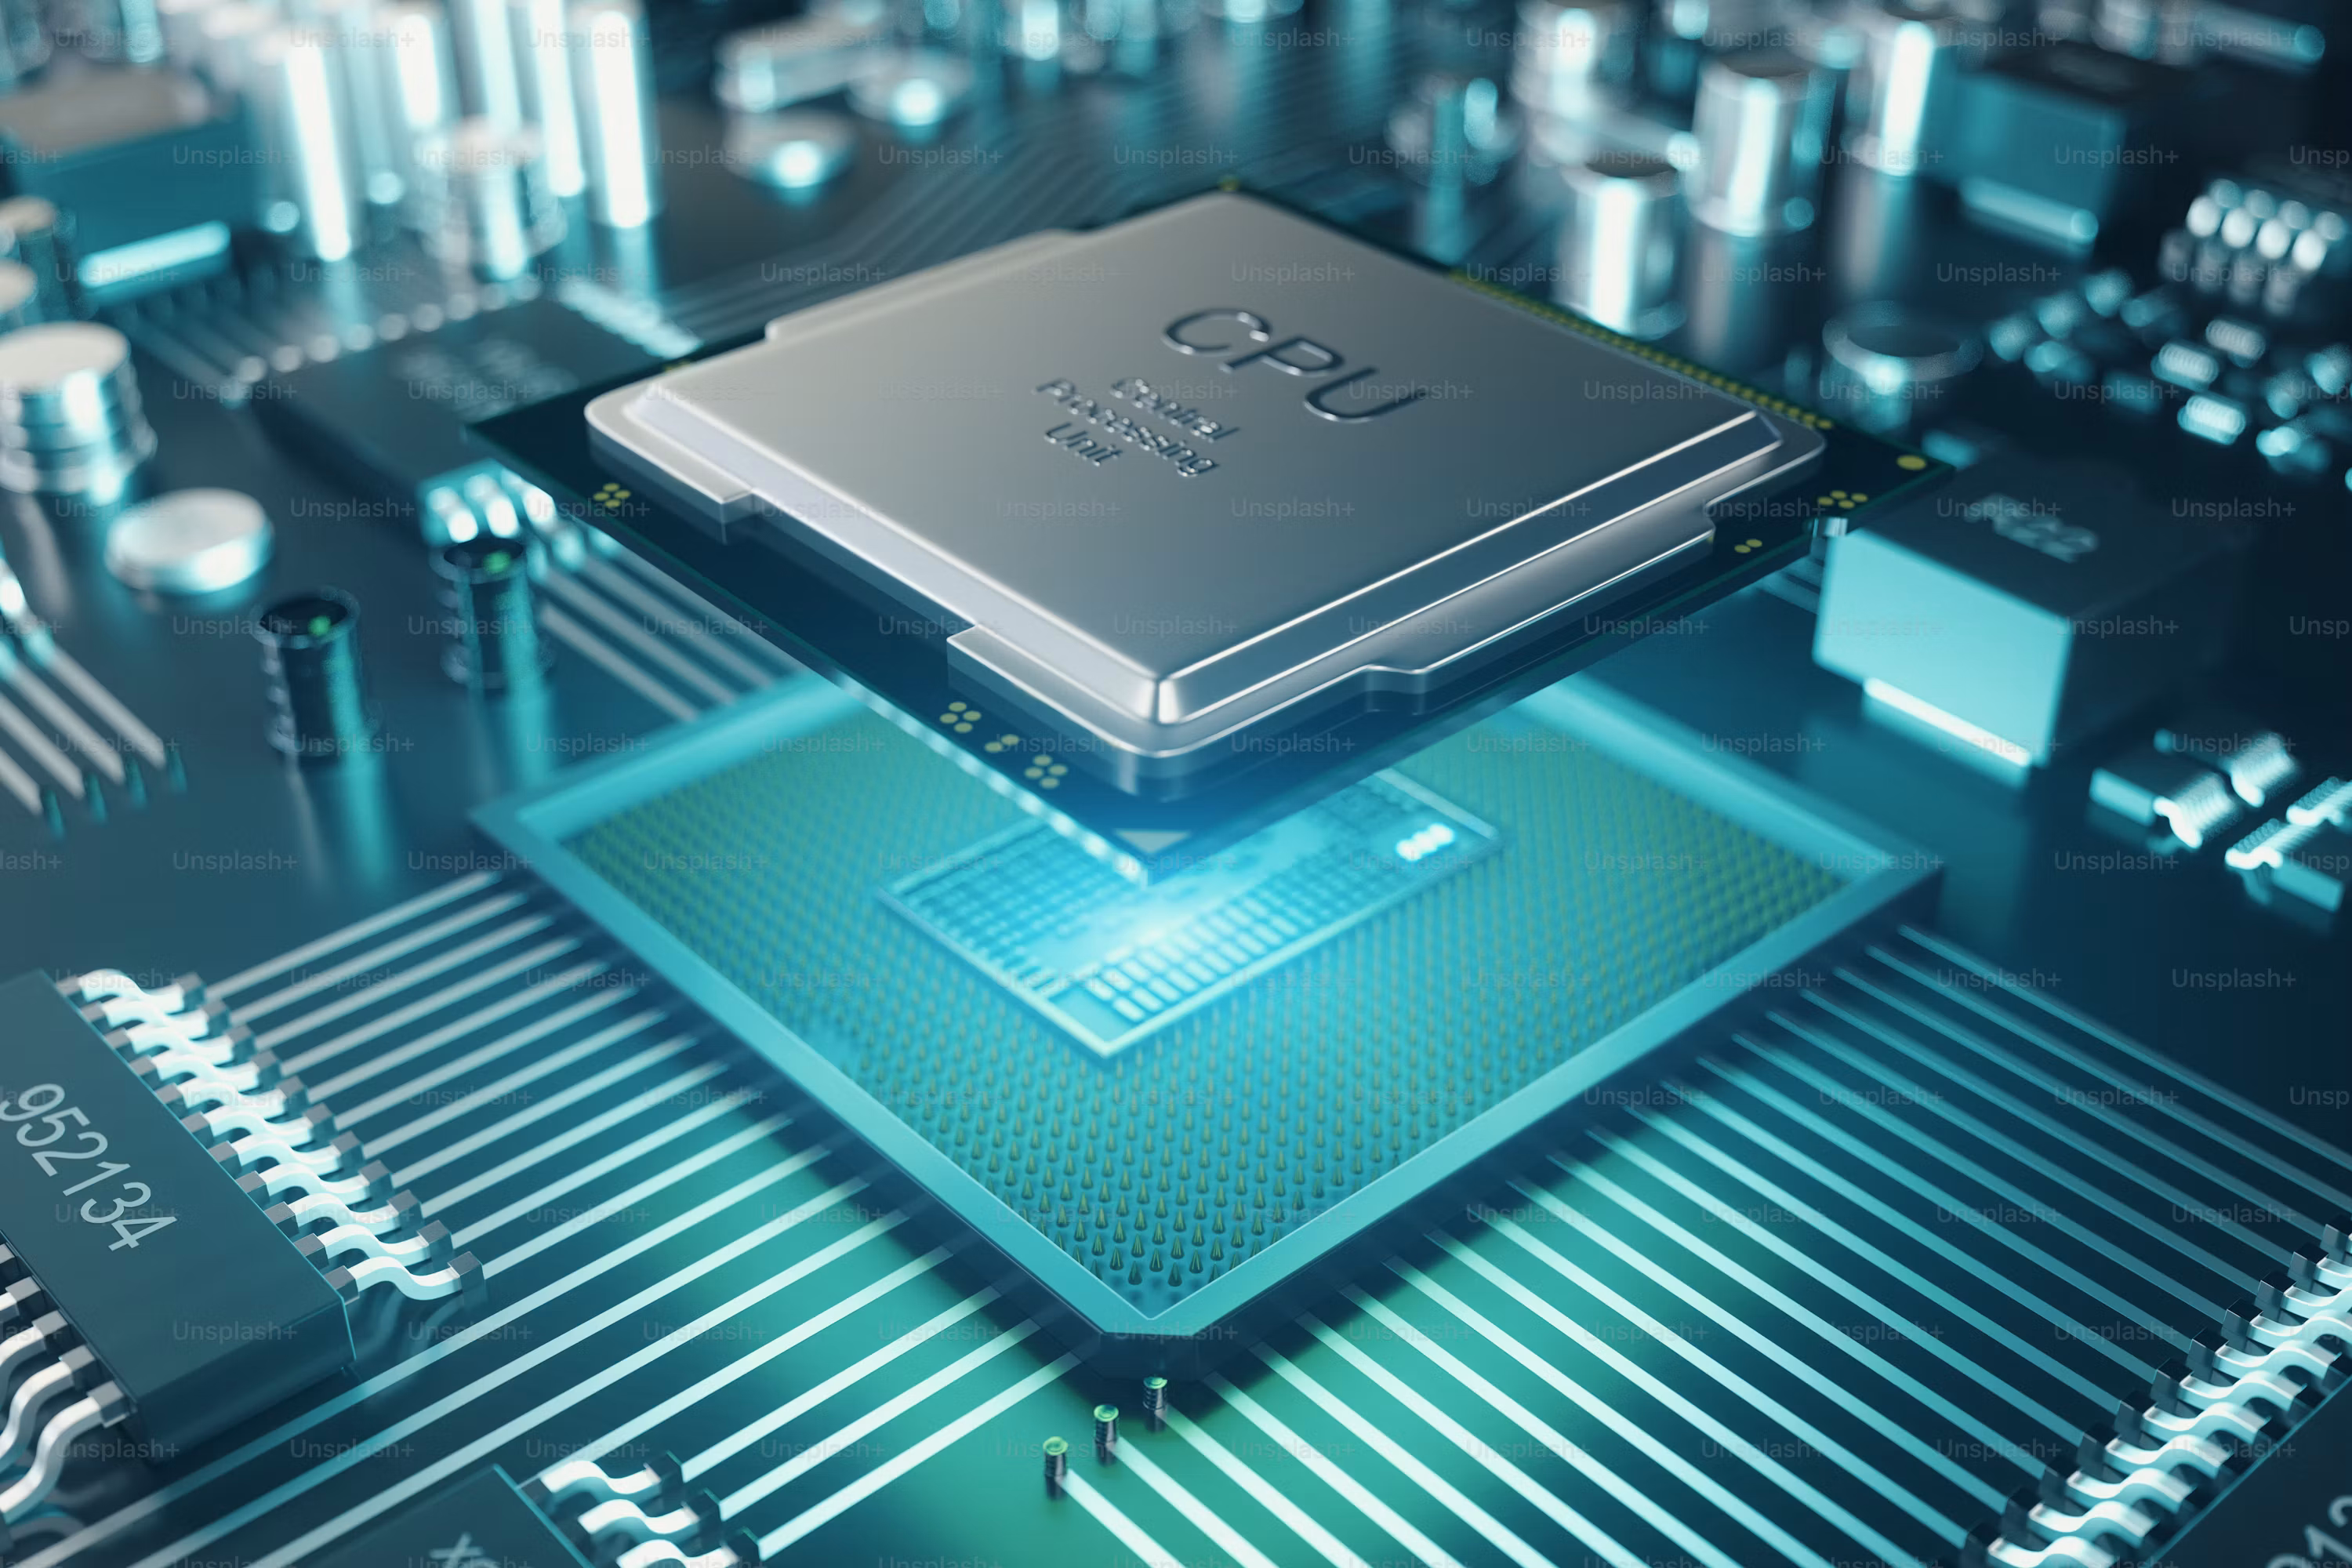
\includegraphics[height=1cm]{Images/top.png}} 
\fancyhead[R]{\thepage} 
\fancyhead[C]{\textit{\leftmark}} 

% Per avere l'intestazione anche nelle pagine iniziali dei capitoli
\fancypagestyle{plain}{
  \fancyhf{}
  \fancyhead[L]{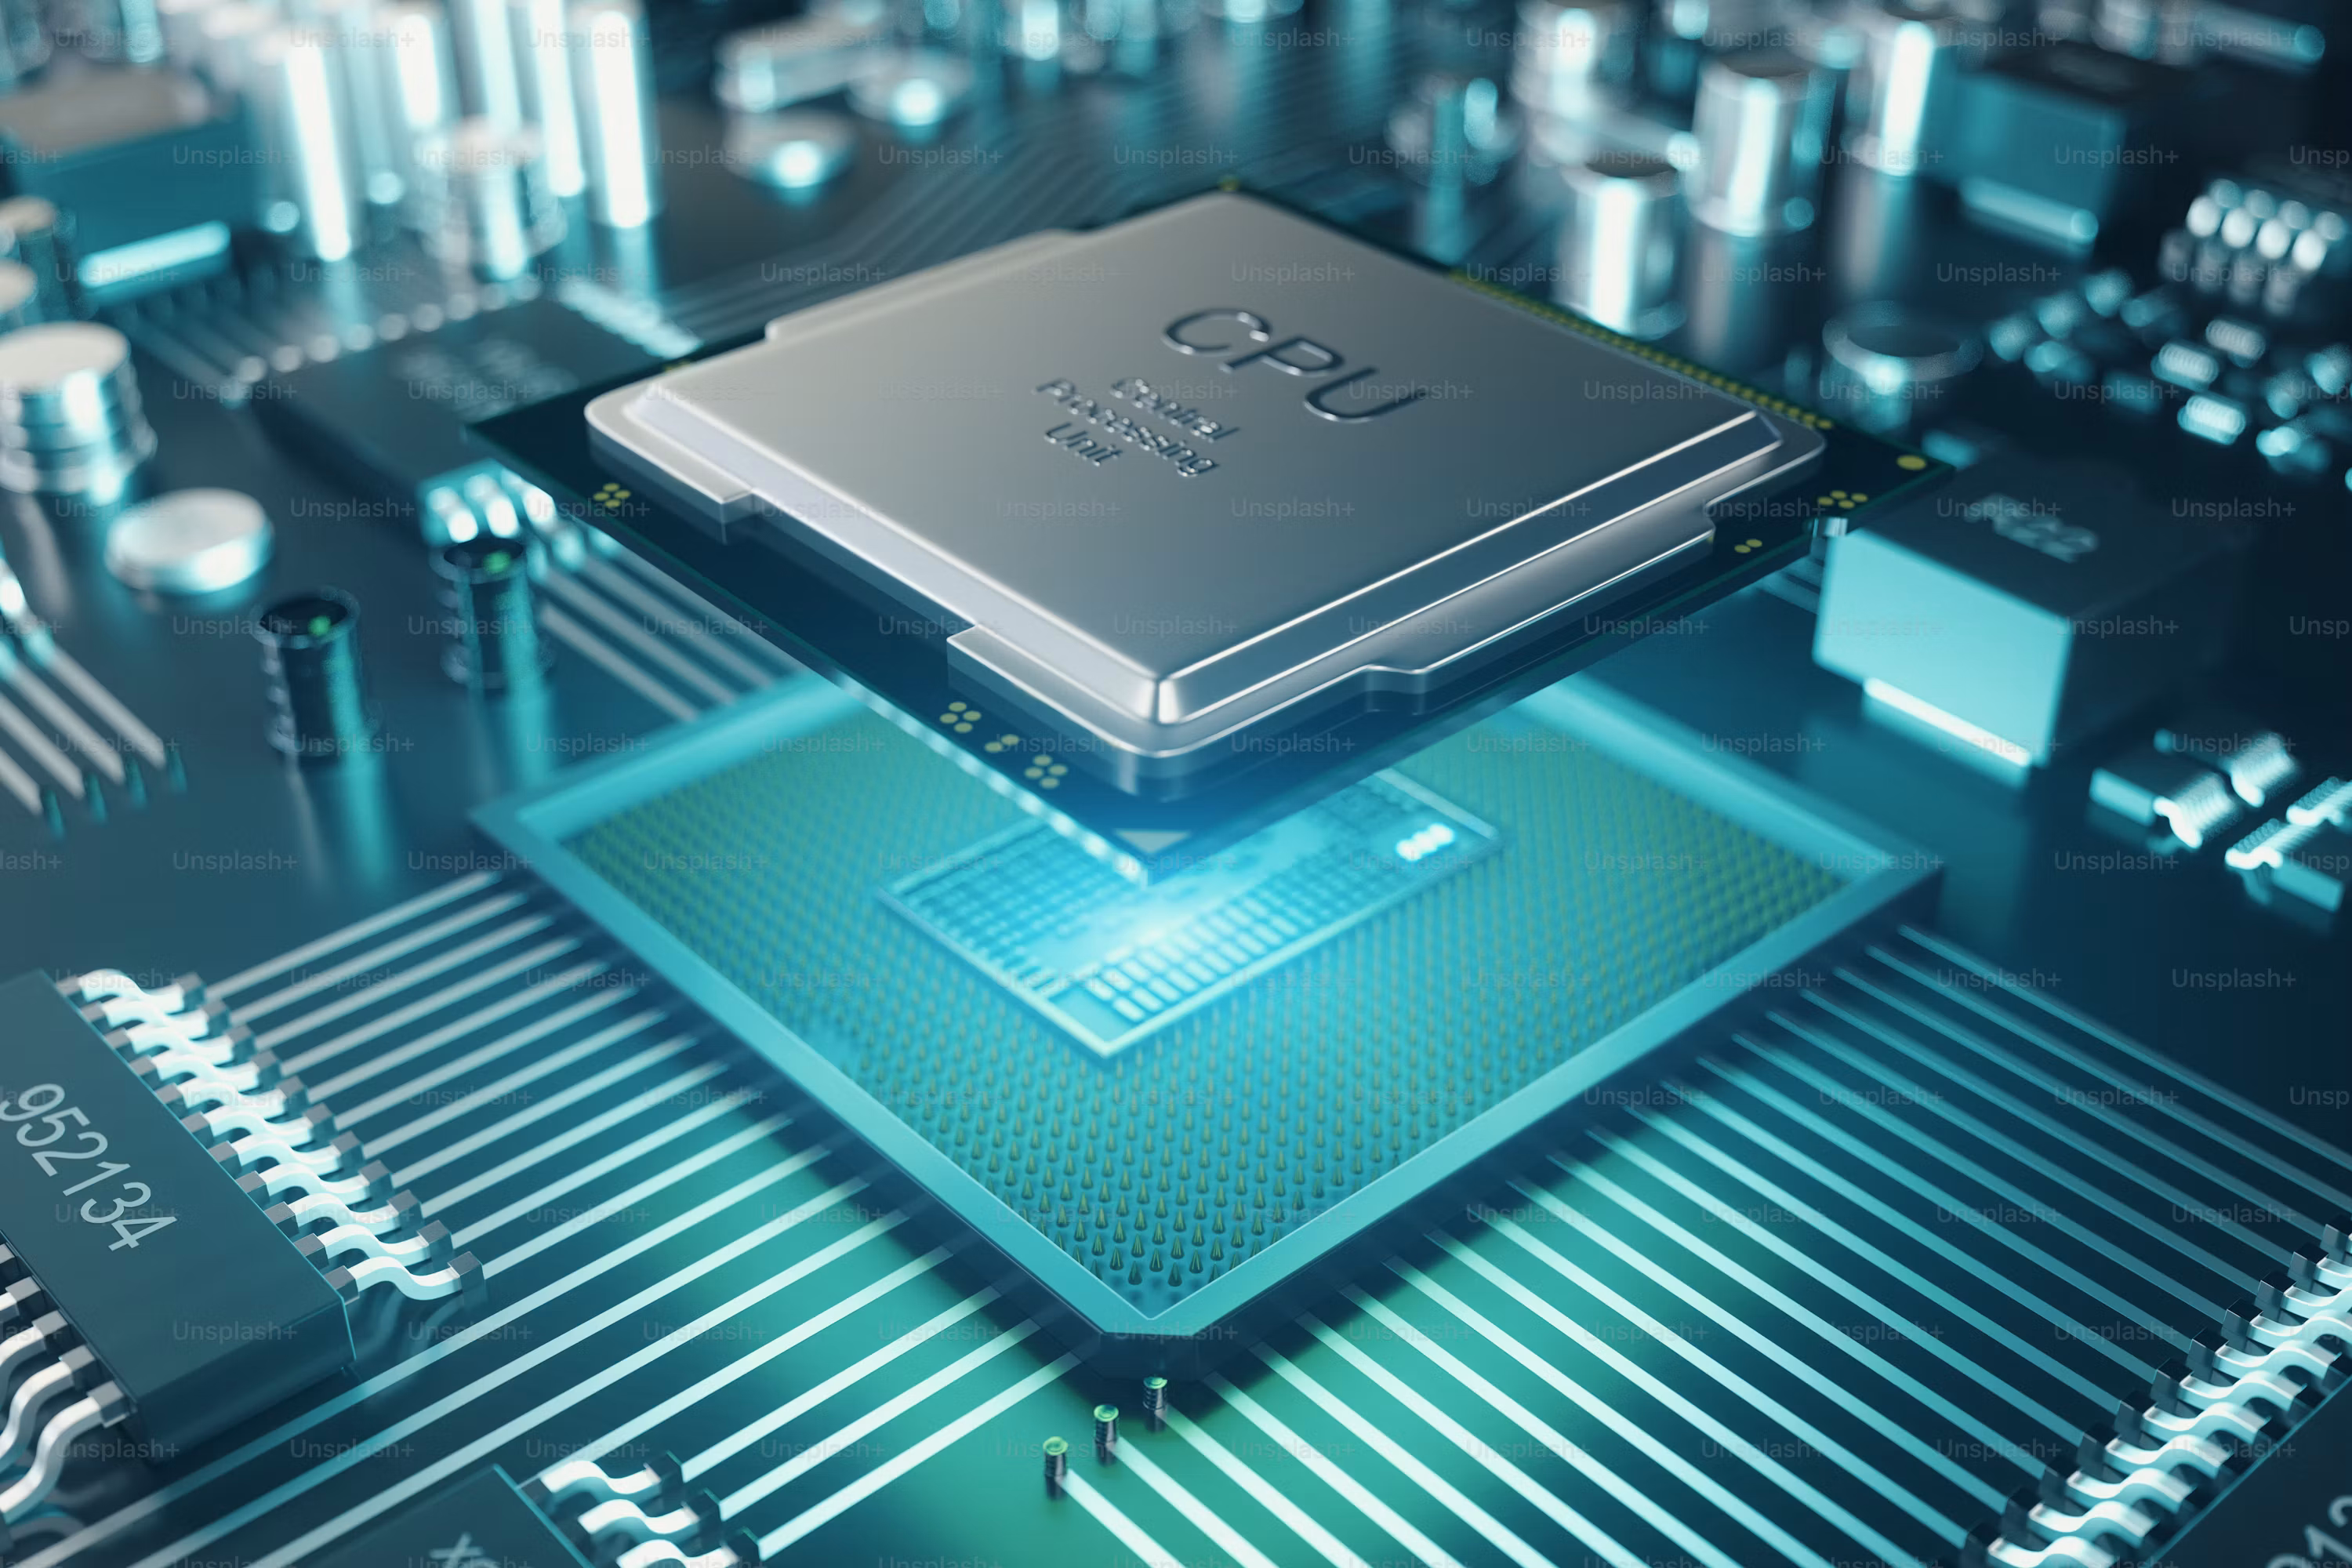
\includegraphics[height=1cm]{Images/top.png}}
  \fancyhead[R]{\thepage}
  \fancyhead[C]{\textit{\leftmark}}
  \renewcommand{\headrulewidth}{0.4pt}
}

% --- LINK CLICCABILI (Senza il backtick d'errore) ---
\usepackage[hidelinks]{hyperref} 
 

% --- COMANDI PERSONALIZZATI ---
\newcommand{\tikznode}[2]{%
  \ifmmode%
    \tikz[remember picture,baseline=(#1.base),inner sep=0pt] \node (#1) {$#2$};%
  \else
    \tikz[remember picture,baseline=(#1.base),inner sep=0pt] \node (#1) {#2};%
  \fi%
}
\tikzset{portnode/.style={circle, draw, inner sep=1pt, font=\scriptsize}}


\begin{document}
% --- PAGINA DEL TITOLO 
\begin{titlepage}
    \centering
    {\scshape\Large Università degli Studi "La Sapienza" \par} 
    \vspace{0.5cm}
    {\scshape\large Dipartimento di Ingegneria dell'Informazione, Elettronica e Telecomunicazioni \par}
    \vspace{0.5cm}
    {\scshape\large Corso di Laurea in Ingegneria Elettronica \par}
    \vspace{1.5cm}
    {\huge\bfseries Laboratorio Multidisciplinare\\ di Elettronica I\par}
    \vspace{0.35cm}
    {\Large\bfseries Relazione \NumeroRelazione\par}
    \vspace{0.35cm}
    {\Large\bfseries \TitoloRelazione\par}
    \vspace{1cm}
    {\large CFU:  6 \par} 
    \vspace{2.5cm}

    {\large Gruppo 18: \par}
    \vspace{0.2cm}
    {\Large Renato Bearzotti \par}
    {\Large Nicolò Falasca \par}

    \vspace{0.8cm}
    \IfFileExists{Images/top.png}{%
        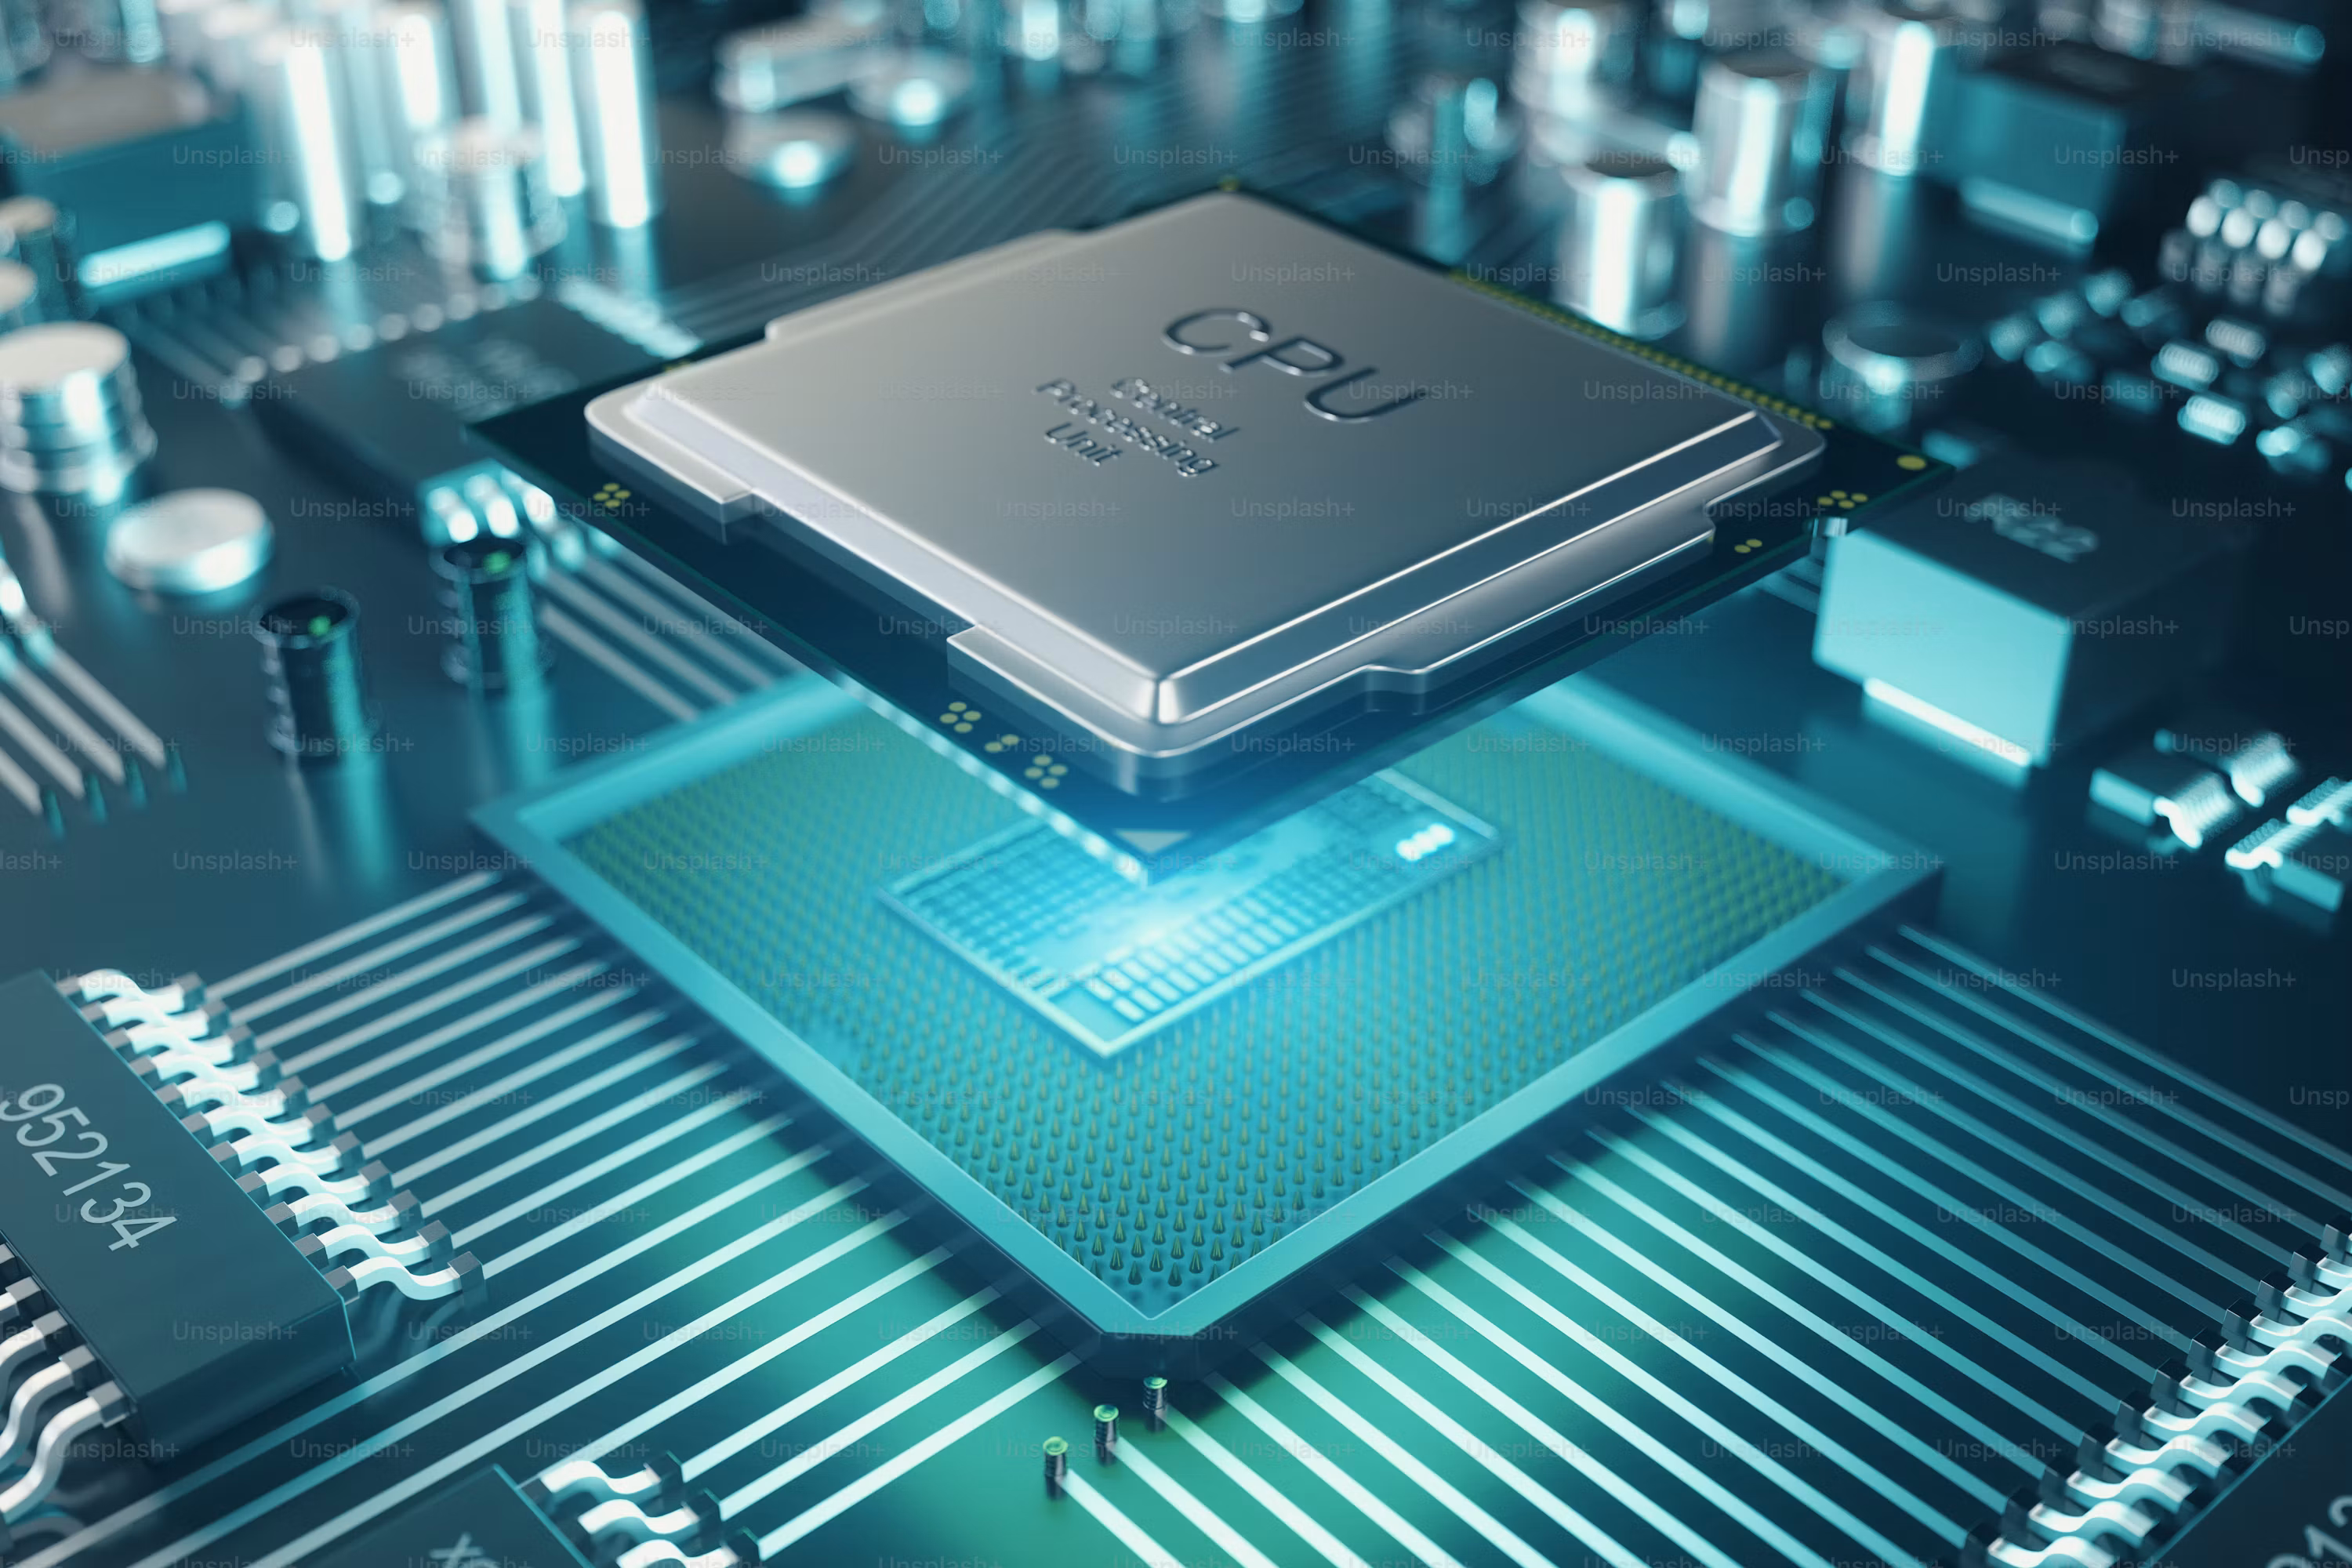
\includegraphics[width=3.5cm]{Images/top.png}\par
    }{}
    \vspace{0.35cm}
    \IfFileExists{Images/logo Sapienza (rgb).png}{%
        
\includegraphics[width=6.8cm]{Images/logo Sapienza (rgb).png}\par
    }{}
    \vspace{0.8cm}

    % Professori allineati a destra
    \begin{minipage}[t]{\textwidth}
        \begin{flushright}
            \large
            \textbf{Professori:}\\
            Andrea Mostacci\\
            Stefano Pisa\\
            Pasquale Tommasino
        \end{flushright}
    \end{minipage}

    \vfill
    {\large Anno Accademico 2026-2027 \par}
\end{titlepage}


\frontmatter
\tableofcontents

\mainmatter

\chapter{Modello in trasmissione e ricerca dei modi}
\chaptermark{Modello in trasmissione}

In questa esercitazione abbiamo misurato in trasmissione una cavità a due celle, collegata con due cavi coassiali alle due porte dell'analizzatore di reti FieldFox. La cavità ha due antenne che si possono inserire ed estrarre e due tuner a vite, e tutte e tre le parti della practice sono state svolte su di essa: nella prima parte abbiamo misurato i suoi quattro modi fra 1.5 e 3.1\,GHz, nella seconda abbiamo studiato l'effetto dei tuner sul primo modo e nella terza abbiamo variato l'accoppiamento delle antenne sul secondo modo.

Per ognuno dei quattro modi la practice chiede di misurare la frequenza di risonanza $f_0$ e il fattore di merito caricato $Q_L$, sia dal modulo sia dalla fase di $S_{21}$, e per i modi sottoaccoppiati anche i coefficienti di accoppiamento $\beta_1$, $\beta_2$ delle due antenne e il fattore di merito a vuoto $Q_0$.

\section{Risposta attesa in trasmissione (punto 1.1)}
Dalla teoria sappiamo che attorno a una risonanza la cavità si comporta come un risonatore accoppiato alle due porte tramite le antenne, e che il parametro di trasmissione vale
\begin{equation}
S_{21}(f)=\frac{S_{21}(f_0)}{1+jQ_L\delta},\qquad \delta=\frac{f}{f_0}-\frac{f_0}{f},
\label{eq:S21}
\end{equation}
con
\begin{equation}
S_{21}(f_0)=\frac{2\sqrt{\beta_1\beta_2}}{1+\beta_1+\beta_2},\qquad Q_L=\frac{Q_0}{1+\beta_1+\beta_2},
\label{eq:S21f0}
\end{equation}
dove $\beta_1$ e $\beta_2$ sono i coefficienti di accoppiamento delle due antenne e $Q_0$ è il fattore di merito della cavità senza carico. $S_{21}(f_0)$ è un numero reale: alla risonanza la fase della cavità è nulla.

Dividendo per $S_{21}(f_0)$ si ottiene la curva normalizzata, che dipende solo da $Q_L$ e da $\delta$:
\begin{equation}
\left|\frac{S_{21}(f)}{S_{21}(f_0)}\right|=\frac{1}{\sqrt{1+(Q_L\delta)^2}},\qquad
\left|\frac{S_{21}(f)}{S_{21}(f_0)}\right|_{dB}=-10\log_{10}\left[1+(Q_L\delta)^2\right].
\label{eq:S21norm}
\end{equation}
Nei due punti in cui $Q_L\delta=\pm1$ il modulo è sceso di 3\,dB. Vicino alla risonanza $\delta\simeq 2(f-f_0)/f_0$, quindi i due punti distano $BW=f_0/Q_L$: è la relazione usata dallo strumento per misurare $Q_L$ dalla banda a $-3$\,dB.

La fase di $S_{21}$ è
\begin{equation}
\angle S_{21}(f)=\angle S_{21}(f_0)-\arctan(Q_L\delta)
\label{eq:fase}
\end{equation}
e passa da $+90^\circ$ a $-90^\circ$ attraversando la risonanza. Vicino a $f_0$, cioè per $|Q_L\delta|\ll1$, l'arcotangente si può approssimare con il suo argomento:
\begin{equation}
\angle S_{21}(f)-\angle S_{21}(f_0)\simeq -Q_L\,\delta\simeq-\frac{2Q_L}{f_0}\,(f-f_0).
\label{eq:faselin}
\end{equation}
La fase è quindi lineare attorno a $f_0$, con pendenza $-Q_L$ in funzione di $\delta$ e $-2Q_L/f_0$ in funzione della frequenza: è la relazione che useremo nel capitolo~\ref{cap:fase} per ricavare $Q_L$ dal fit lineare.

\section{Strumento e set-up}
L'analizzatore è il FieldFox (10\,kHz--14\,GHz), con 801 punti per traccia. Le tracce sono state acquisite sul PC con la routine del corso \texttt{DataAquisition12.m}, che tramite \texttt{getdataFFPNA} legge la traccia attiva dello strumento e salva la struttura \texttt{dataStruct} con il vettore delle frequenze, la parte reale e immaginaria del parametro misurato e il dato nel formato dello schermo, cioè MLOG per il modulo in dB e UPH per la fase srotolata. I grafici e i conti di questa relazione sono fatti in MATLAB a partire da questi file.

\begin{figure}[H]
\centering
\begin{tikzpicture}[>={Stealth[length=5pt]},
  box/.style={draw,thick,rounded corners=2pt,minimum height=1.3cm,minimum width=2.8cm,align=center,font=\small}]
  \node[box,minimum width=4.4cm] (ff) at (0,0) {FieldFox\\(10\,kHz--14\,GHz, 801 punti)};
  \node[font=\footnotesize] (p1) at (-1.3,-0.95) {porta 1};
  \node[font=\footnotesize] (p2) at (1.3,-0.95) {porta 2};
  \fill (-1.3,-0.65) circle[radius=2pt]; \fill (1.3,-0.65) circle[radius=2pt];
  % cavita'
  \draw[thick,fill=orange!20] (-1.6,-3.6) rectangle (1.6,-2.4);
  \node[font=\small] at (0,-3.0) {cavità};
  \draw[very thick] (-1.0,-2.4) -- (-1.0,-2.75);
  \draw[very thick] (1.0,-2.4) -- (1.0,-2.75);
  \node[font=\footnotesize,left] at (-1.6,-2.6) {antenna 1};
  \node[font=\footnotesize,right] at (1.6,-2.6) {antenna 2};
  \draw[very thick,gray!70!black,rounded corners=5pt] (-1.3,-0.65) -- (-1.3,-1.6) -- (-1.0,-1.9) -- (-1.0,-2.4);
  \draw[very thick,gray!70!black,rounded corners=5pt] (1.3,-0.65) -- (1.3,-1.6) -- (1.0,-1.9) -- (1.0,-2.4);
  \node[font=\footnotesize,gray!40!black] at (-2.35,-1.65) {cavo coassiale};
  \node[box] (pc) at (5.6,0) {PC con MATLAB\\(\texttt{DataAquisition12})};
  \draw[->,thick] (ff.east) -- node[above,font=\footnotesize]{LAN} (pc.west);
\end{tikzpicture}
\caption{Set-up delle misure in trasmissione: la cavità è collegata alle due porte del FieldFox con due cavi coassiali.}
\label{fig:setup}
\end{figure}

Per misurare solo $f_0$ e $Q_L$ la calibrazione non è necessaria, ma serve se si vuole confrontare il valore misurato di $S_{21}(f_0)$ con la (\ref{eq:S21f0}). Nella prima parte la calibrazione non risultava attiva, come si vede dai dati: lontano dalla risonanza $|S_{11}|$ e $|S_{22}|$ valgono circa $-2.6$ e $-3.2$\,dB invece di 0\,dB, e la fase di $S_{21}$ scende con una pendenza che corrisponde a un ritardo di circa 19\,ns. I cavi restano quindi dentro la misura; ne terremo conto nei capitoli~\ref{cap:fase} e~\ref{cap:beta}.

\section{Ricerca dei quattro modi}
Come ci è stato indicato in laboratorio, i modi si possono cercare anche senza calibrazione, quindi per prima cosa abbiamo misurato $|S_{21}|$ su uno span largo, da 1.5 a 3.3\,GHz. Con 801 punti su 1.8\,GHz due punti distano 2.25\,MHz: è troppo per misurare le risonanze, che sono larghe qualche centinaio di kHz, ma basta per vedere dove si trovano. Il grafico è il seguente:

\begin{figure}[H]
\centering
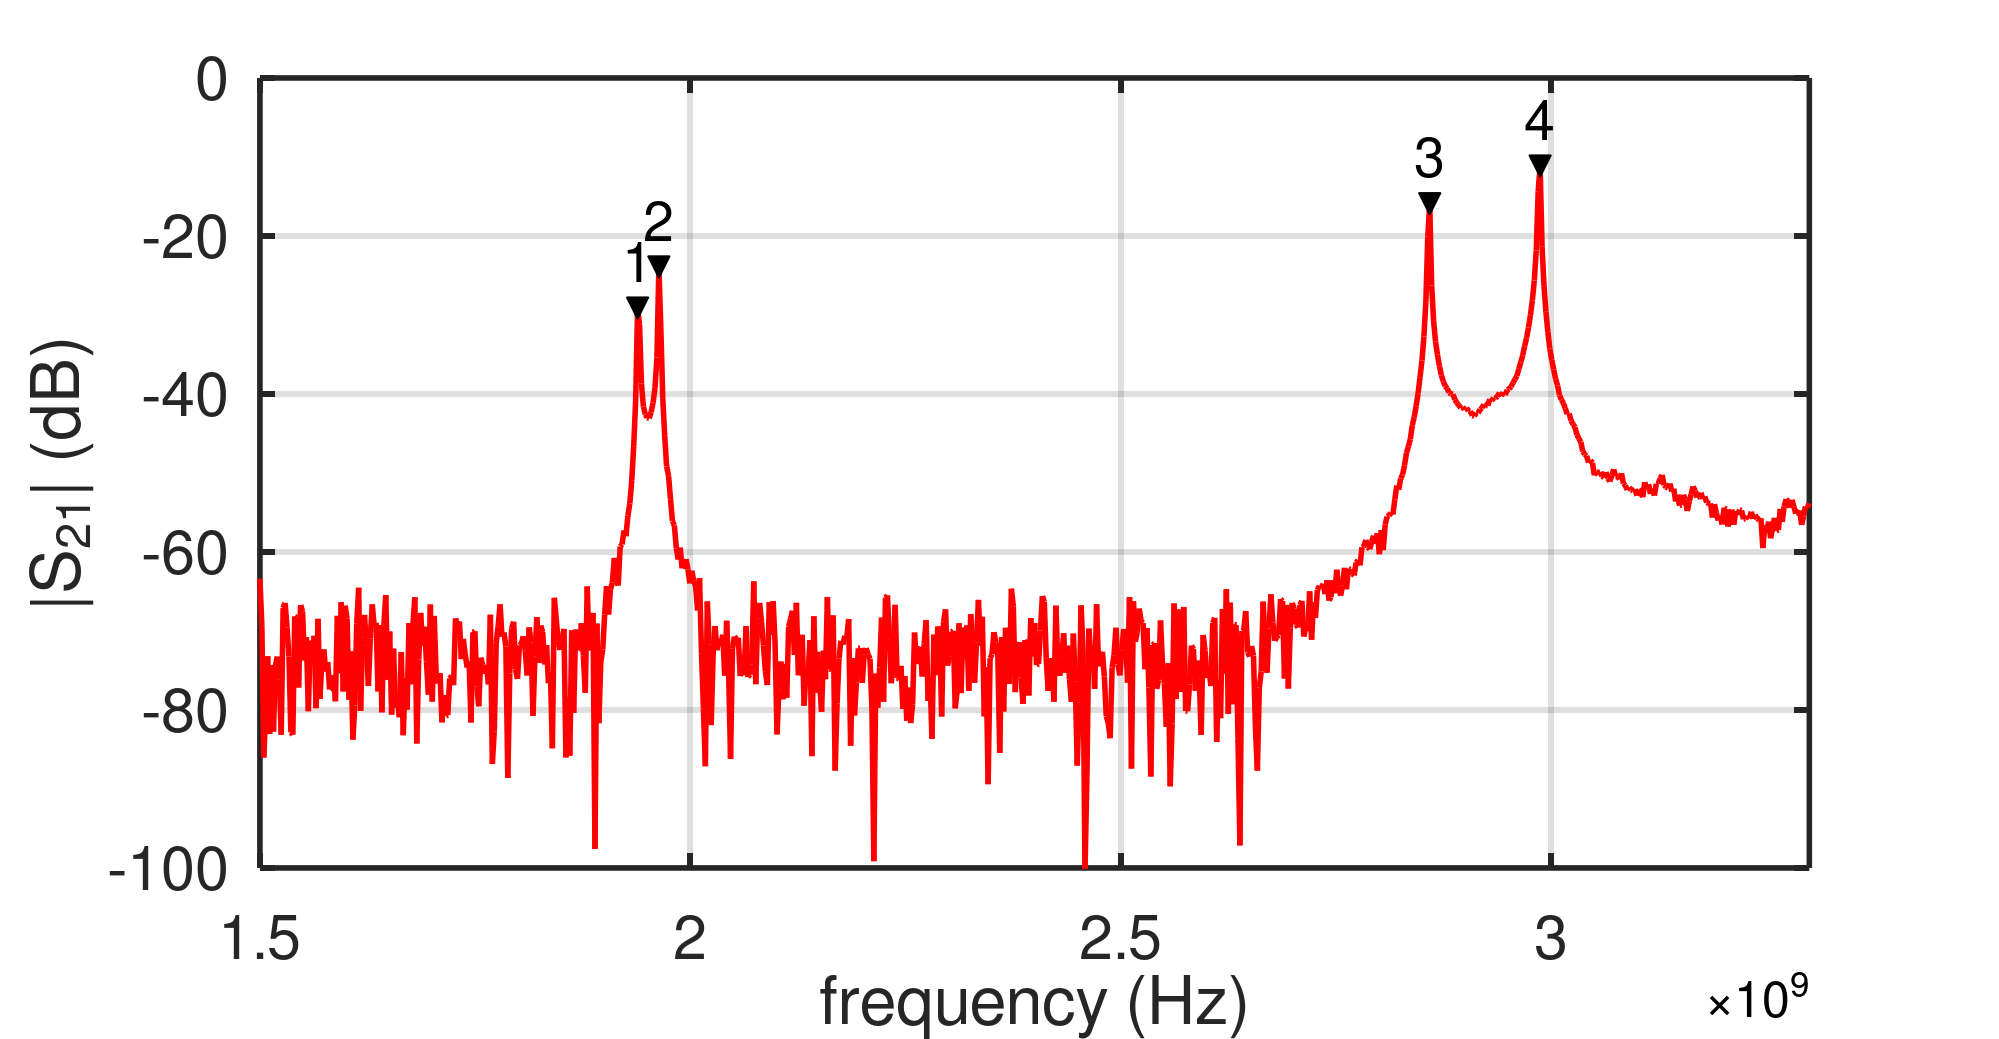
\includegraphics[width=0.95\textwidth]{Images/Relazione6_Foto/fig_1_1_quattro_modi.png}
\caption{Modulo di $S_{21}$ da 1.5 a 3.3\,GHz: i quattro modi della cavità.}
\label{fig:4modi}
\end{figure}

Come si può notare i picchi sono quattro e vengono a coppie: due attorno a 1.95\,GHz, distanti circa 25\,MHz, e due attorno a 2.9\,GHz, distanti circa 128\,MHz. Questo è coerente con una cavità a due celle, in cui i modi della singola cella si dividono in coppie, con le due celle che oscillano in fase o in controfase. Fra 1.5 e 2.7\,GHz, lontano dai modi, $|S_{21}|$ è al livello del rumore, fra $-100$ e $-63$\,dB. Fra il terzo e il quarto modo e oltre il quarto la traccia resta più alta, fra $-40$ e $-60$\,dB, per le code dei due modi. Su ogni picco abbiamo messo il marker con \emph{Peak Search} e, dopo averlo portato al centro dello schermo, abbiamo ristretto lo span per le misure successive. Le frequenze dei picchi lette con il marker sono in tabella~\ref{tab:modi}.

\begin{table}[H]
\centering
\renewcommand{\arraystretch}{1.2}
\begin{tabular}{c c c c}
\hline
modo & $f$ del picco [GHz] & $|S_{21}|$ al picco [dB] & span usato \\ \hline
1 & 1.93966 & $-10.8$ & 8\,MHz \\
2 & 1.96423 & $-9.8$ & 30\,MHz \\
3 & 2.85816 & $-7.4$ & 30\,MHz \\
4 & 2.98640 & $-5.8$ & 30\,MHz \\ \hline
\end{tabular}
\caption{Frequenze dei quattro modi lette con il marker e span delle misure successive.}
\label{tab:modi}
\end{table}

\chapter{Misura di $f_0$ e $Q_L$ dal modulo di $S_{21}$}
\label{cap:modulo}

Per ogni modo abbiamo acquisito modulo e fase di $S_{21}$ in un intervallo di frequenza centrato sulla risonanza e abbastanza largo da far vedere bene la forma attesa, come chiede il punto 1.2, e abbiamo misurato $f_0$ e $Q_L$ dal modulo. Siamo passati poi a confrontare la misura con la curva teorica (\ref{eq:S21norm}) calcolata con i valori misurati, come chiede il punto 1.3.

\section{Metodo e incertezza}
Per $f_0$ e $Q_L$ abbiamo usato la misura automatica del FieldFox, che si trova in \emph{Mark}$\rightarrow$\emph{/Tool}, \emph{Marker Search}, \emph{Bandwidth}: lo strumento cerca il massimo di $|S_{21}|$, trova le due frequenze $f_1$ e $f_2$ a 3\,dB sotto il massimo e restituisce
\begin{equation}
f_0=\frac{f_1+f_2}{2},\qquad BW=f_2-f_1,\qquad Q_L=\frac{f_0}{BW}.
\label{eq:banda}
\end{equation}
Successivamente lo stesso calcolo è stato rifatto in MATLAB sulle tracce salvate, con la funzione \texttt{p6\_banda3dB} che interpola linearmente in dB fra i due punti a cavallo della soglia. I valori che otteniamo coincidono con quelli letti sullo strumento entro lo 0.2\%, come si vede in tabella~\ref{tab:riepilogo}, e nel seguito usiamo quelli calcolati sulle tracce salvate.

L'incertezza principale è dovuta alla risoluzione in frequenza. Con un passo $\Delta f$ fra due punti ciascun estremo della banda è noto a meno di $\pm\Delta f/2$, e considerando una distribuzione uniforme, con $\sigma=\Delta f/\sqrt{12}$ per ciascun estremo, si ha
\begin{equation}
\sigma_{BW}=\frac{\Delta f}{\sqrt6},\qquad \sigma_{f_0}=\frac{\Delta f}{\sqrt{24}},\qquad \sigma_{Q_L}=Q_L\,\frac{\sigma_{BW}}{BW}.
\label{eq:incbanda}
\end{equation}
Il rumore della traccia vicino al picco è dell'ordine del centesimo di dB e sposta i punti a $-3$\,dB molto meno di $\Delta f$, quindi lo trascuriamo.

\section{Modulo e fase dei quattro modi (punto 1.2)}
Nelle figure~\ref{fig:m1}--\ref{fig:m4} sono riportati, per ciascun modo, il modulo di $S_{21}$ in dB a sinistra, con il marker sul massimo, e la fase in formato \emph{Unwrapped Phase} a destra. Come ci aspettavamo il modulo ha la forma a campana e la fase scende di circa $180^\circ$ attraversando la risonanza, come previsto dalla (\ref{eq:fase}). Lontano dalla risonanza la fase continua a scendere linearmente: è il ritardo dei cavi, che senza calibrazione resta nella misura.

\begin{figure}[H]
\centering
\begin{subfigure}{0.49\textwidth}\centering
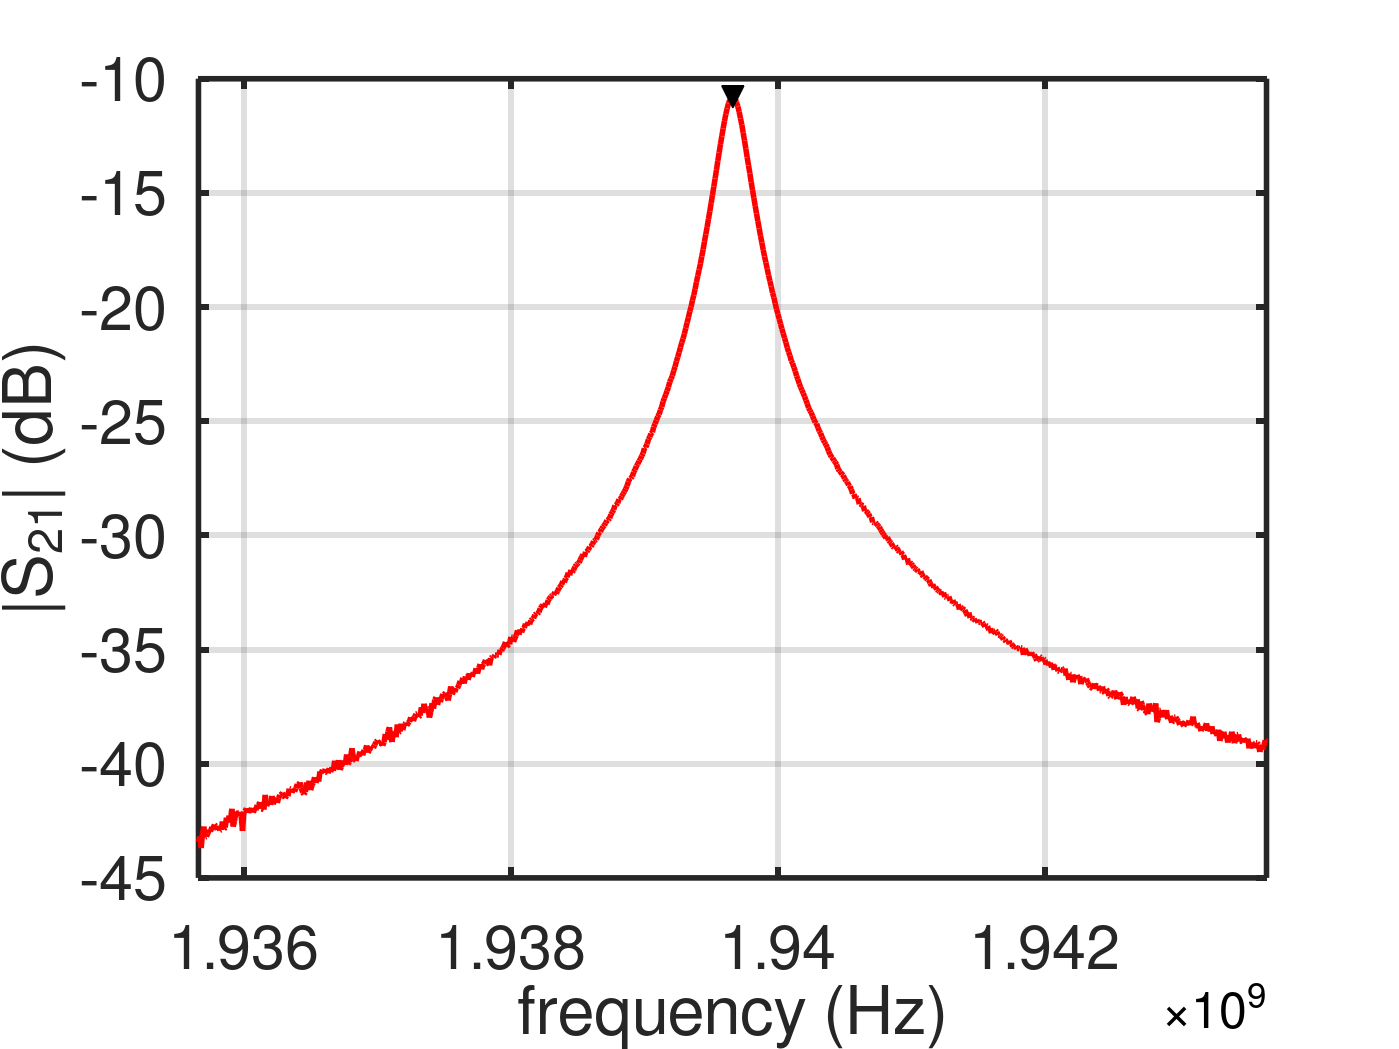
\includegraphics[width=\textwidth]{Images/Relazione6_Foto/fig_1_2_modo1_modulo.png}
\caption{modulo (span 8\,MHz)}
\end{subfigure}
\begin{subfigure}{0.49\textwidth}\centering
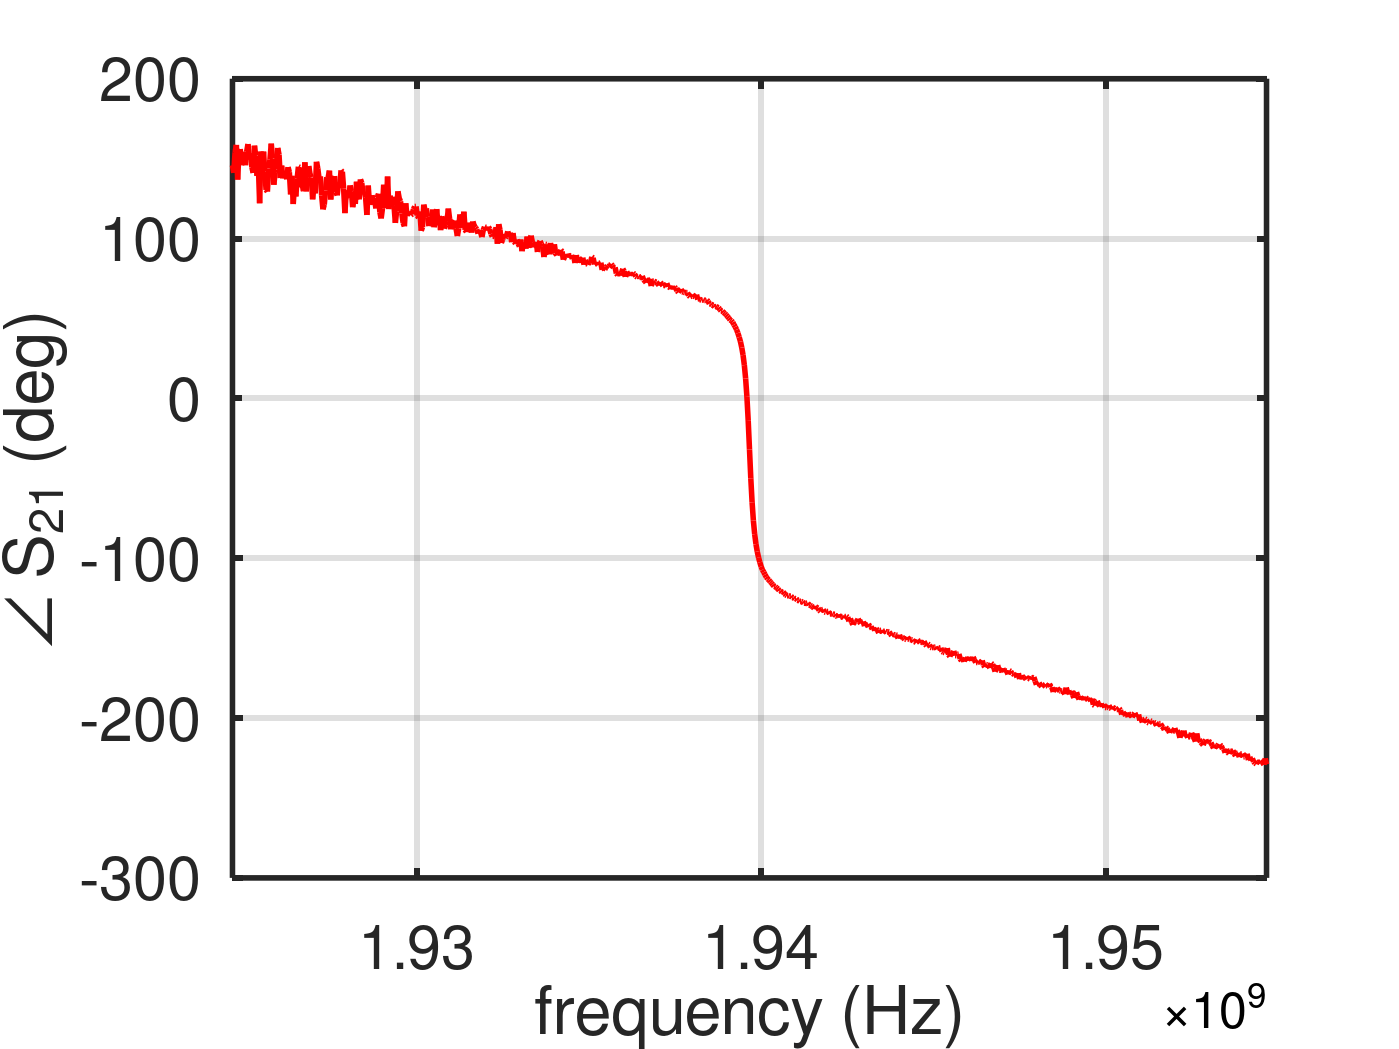
\includegraphics[width=\textwidth]{Images/Relazione6_Foto/fig_1_2_modo1_fase.png}
\caption{fase (span 30\,MHz)}
\end{subfigure}
\caption{Modo 1: modulo e fase di $S_{21}$.}
\label{fig:m1}
\end{figure}

\begin{figure}[H]
\centering
\begin{subfigure}{0.49\textwidth}\centering
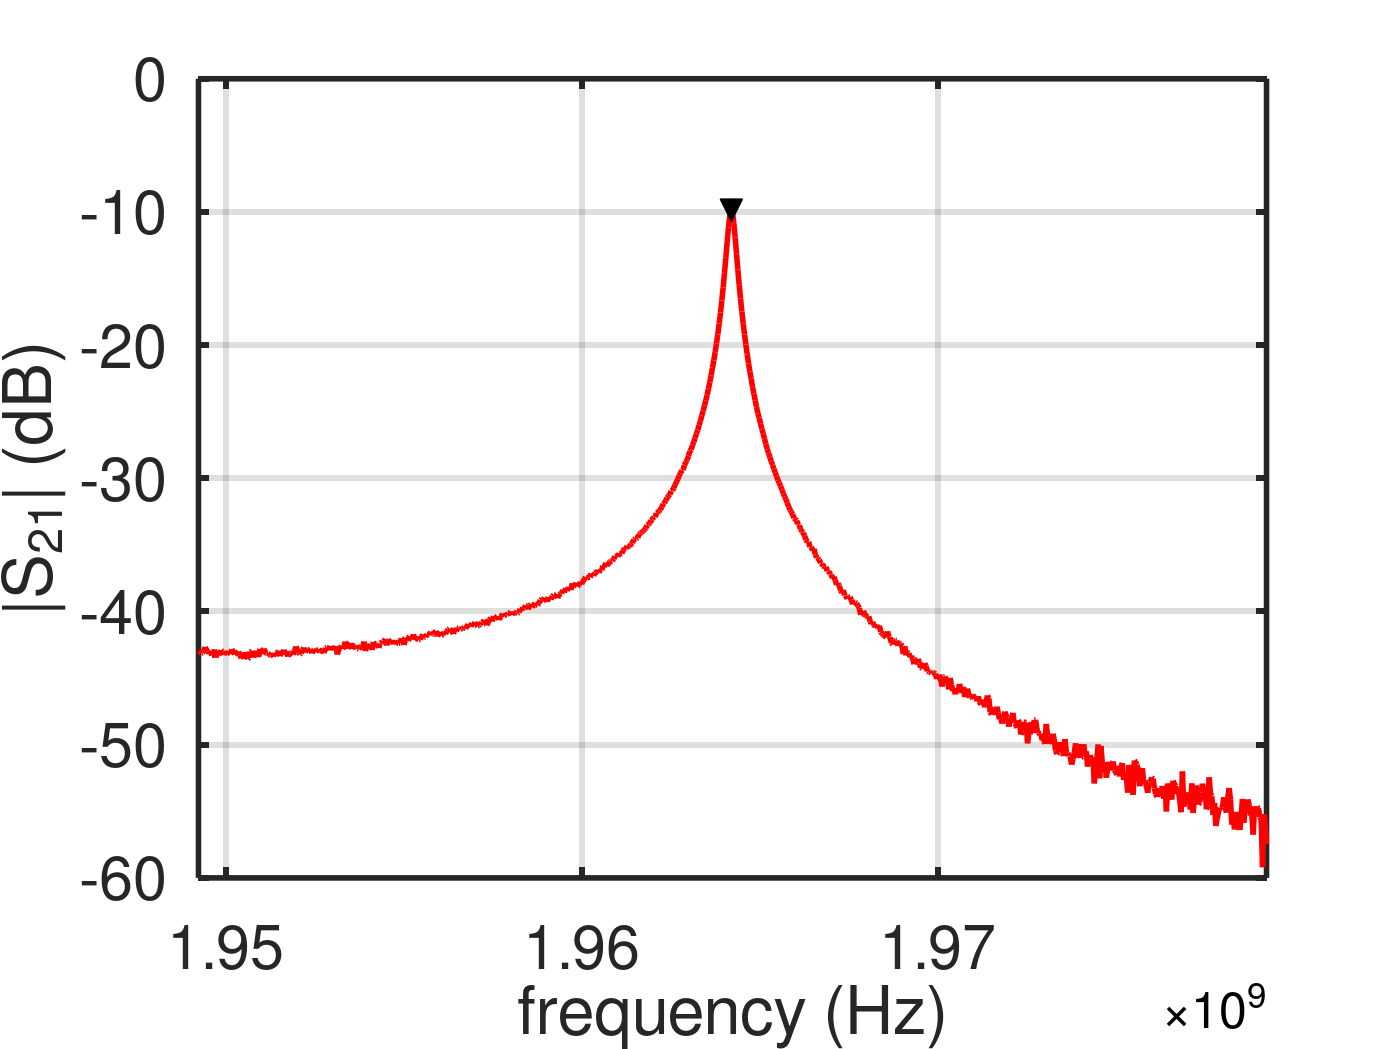
\includegraphics[width=\textwidth]{Images/Relazione6_Foto/fig_1_2_modo2_modulo.png}
\caption{modulo}
\end{subfigure}
\begin{subfigure}{0.49\textwidth}\centering
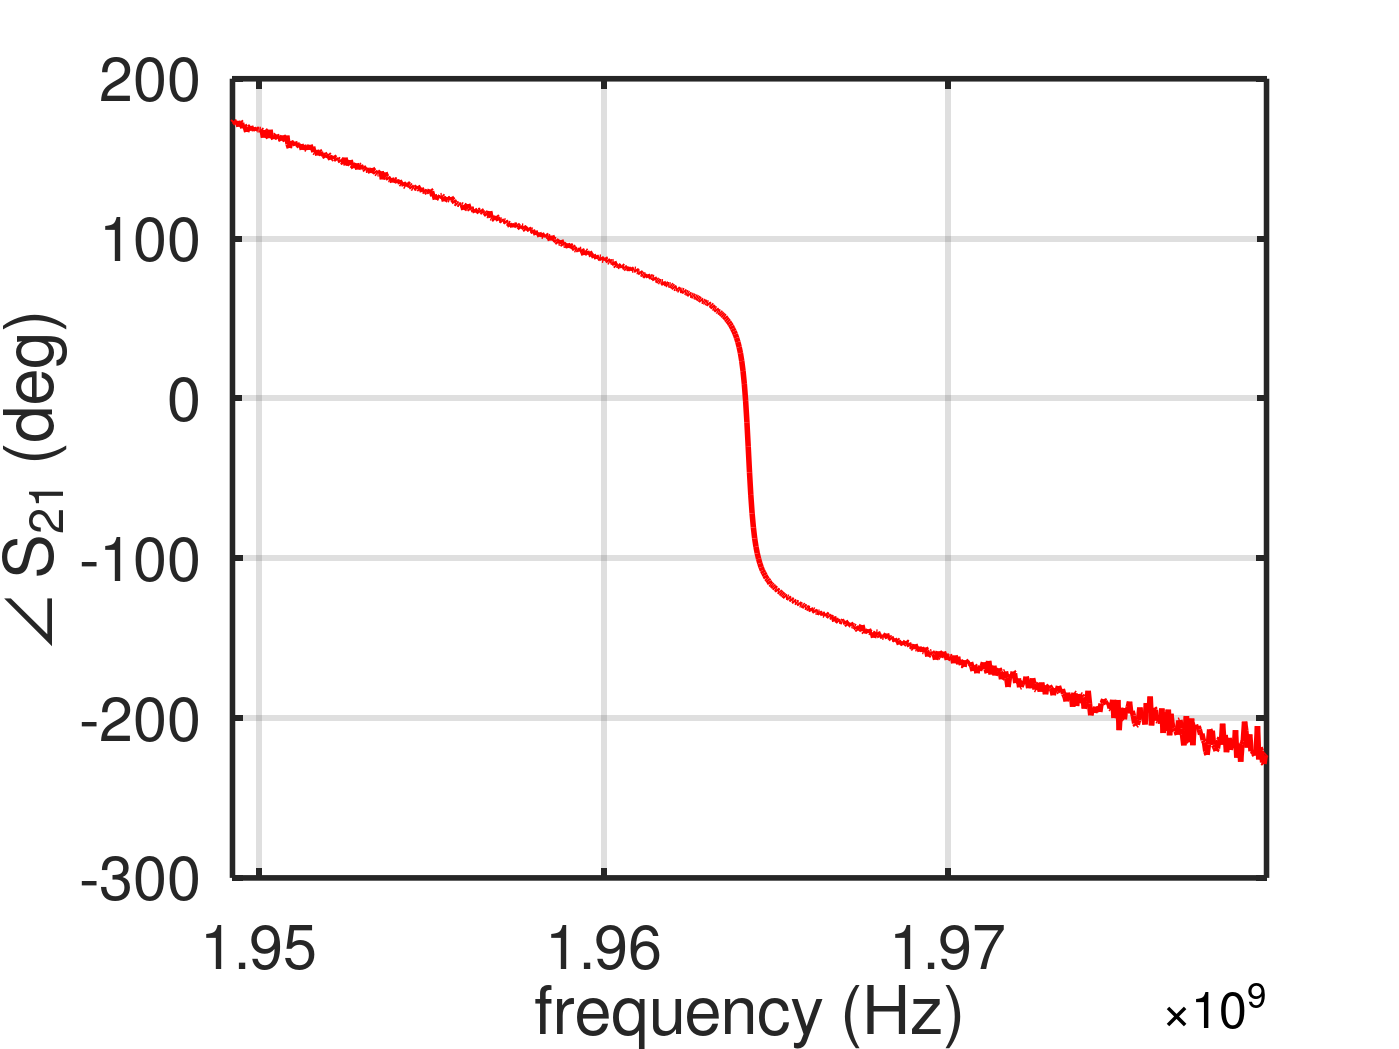
\includegraphics[width=\textwidth]{Images/Relazione6_Foto/fig_1_2_modo2_fase.png}
\caption{fase}
\end{subfigure}
\caption{Modo 2: modulo e fase di $S_{21}$ (span 30\,MHz).}
\label{fig:m2}
\end{figure}

\begin{figure}[H]
\centering
\begin{subfigure}{0.49\textwidth}\centering
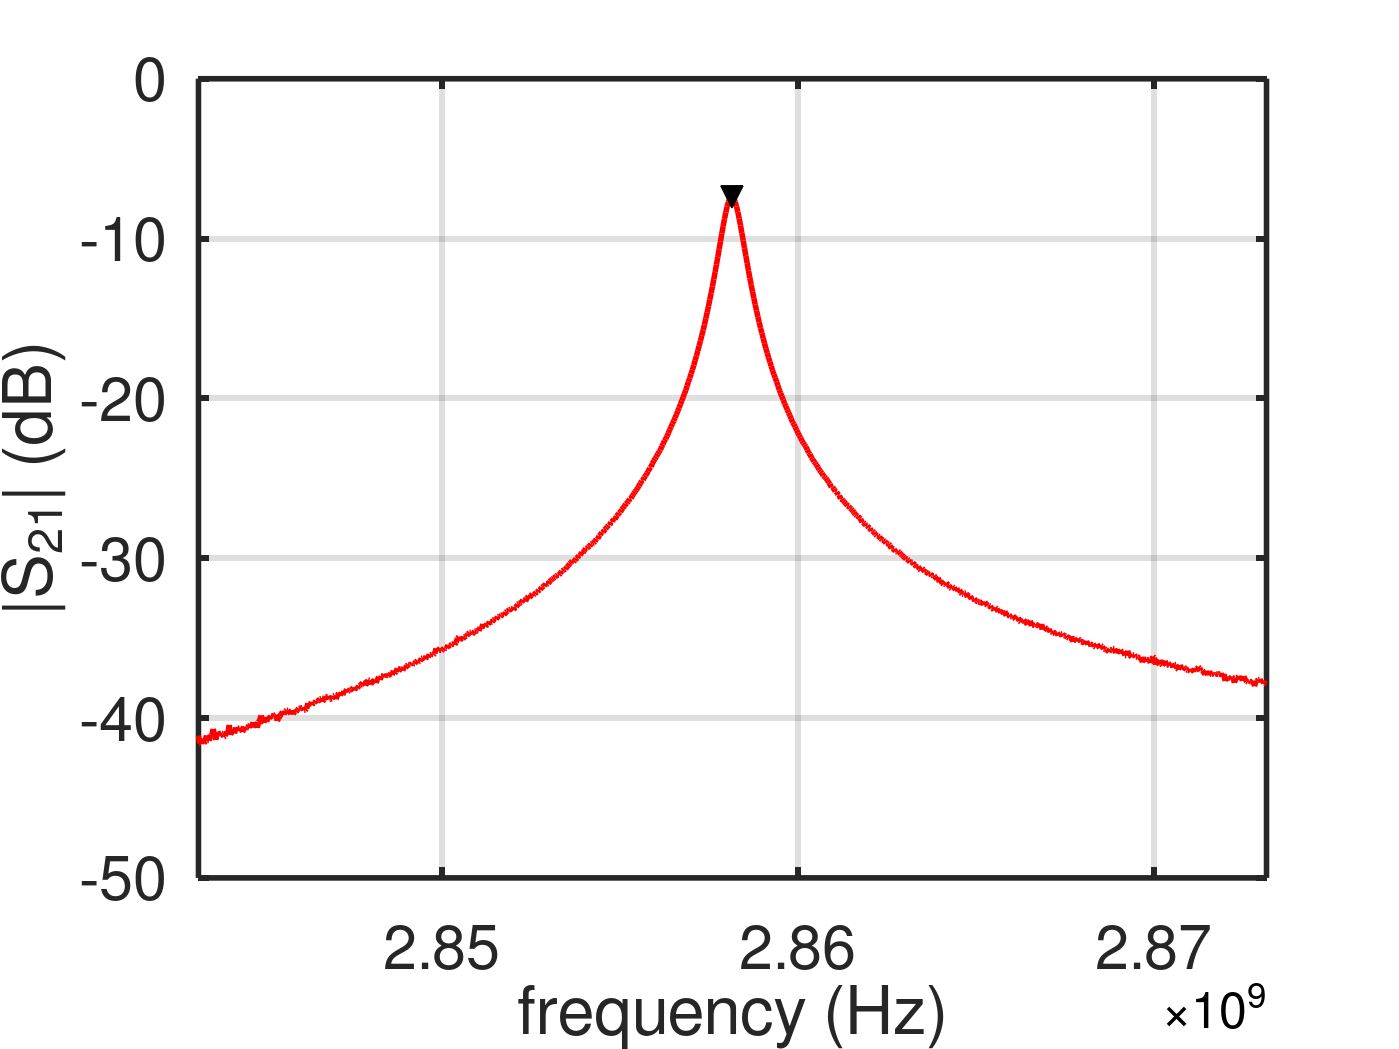
\includegraphics[width=\textwidth]{Images/Relazione6_Foto/fig_1_2_modo3_modulo.png}
\caption{modulo}
\end{subfigure}
\begin{subfigure}{0.49\textwidth}\centering
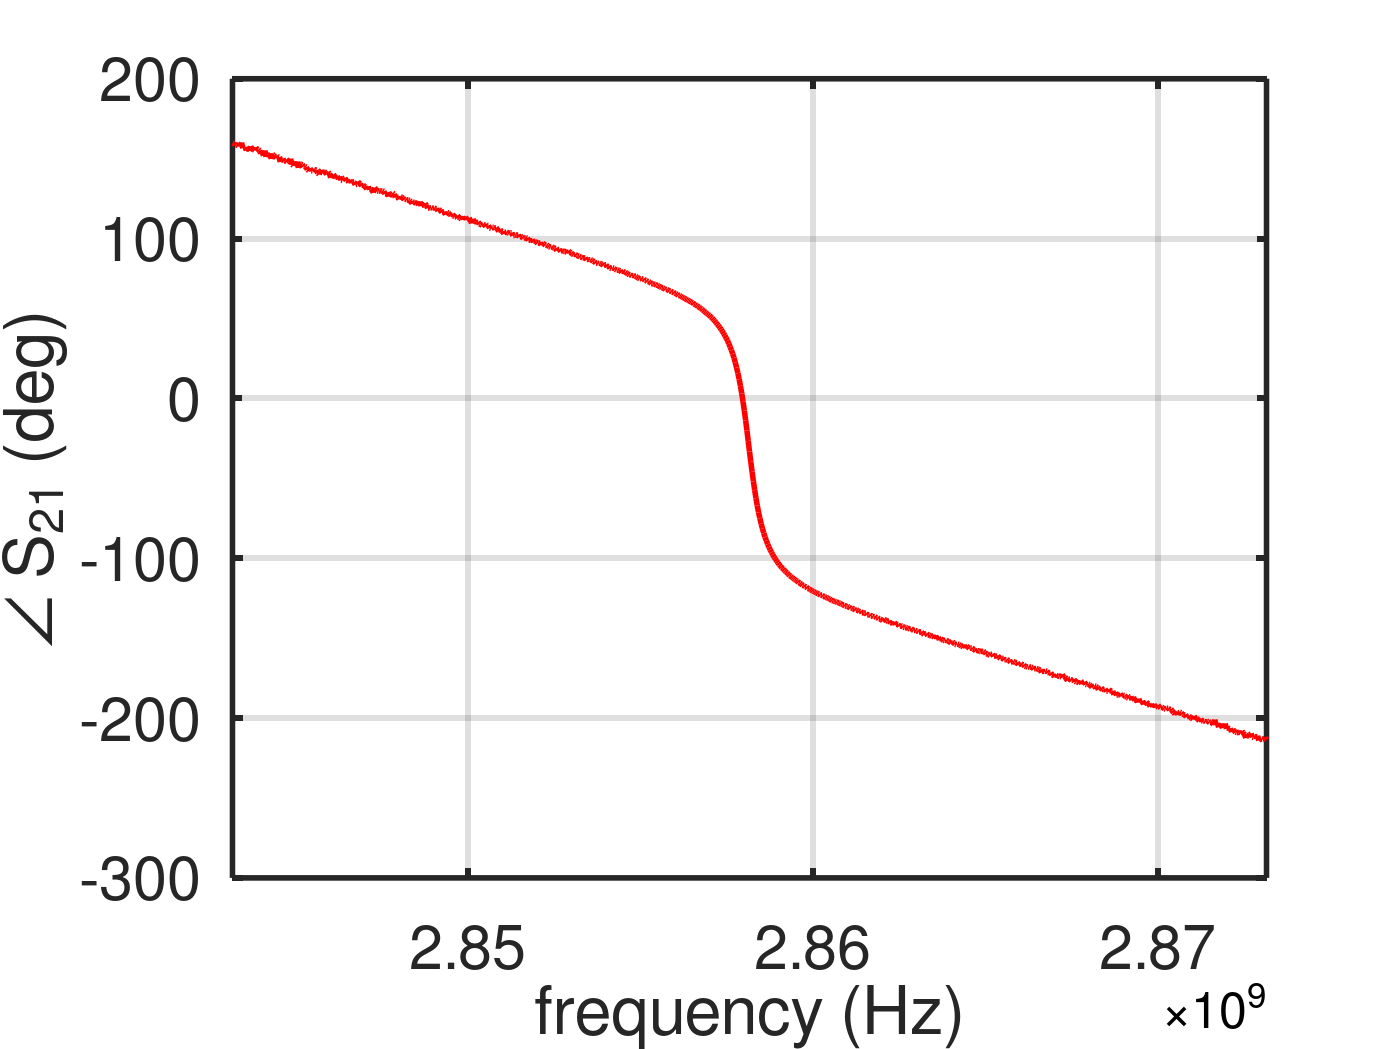
\includegraphics[width=\textwidth]{Images/Relazione6_Foto/fig_1_2_modo3_fase.png}
\caption{fase}
\end{subfigure}
\caption{Modo 3: modulo e fase di $S_{21}$ (span 30\,MHz).}
\label{fig:m3}
\end{figure}

\begin{figure}[H]
\centering
\begin{subfigure}{0.49\textwidth}\centering
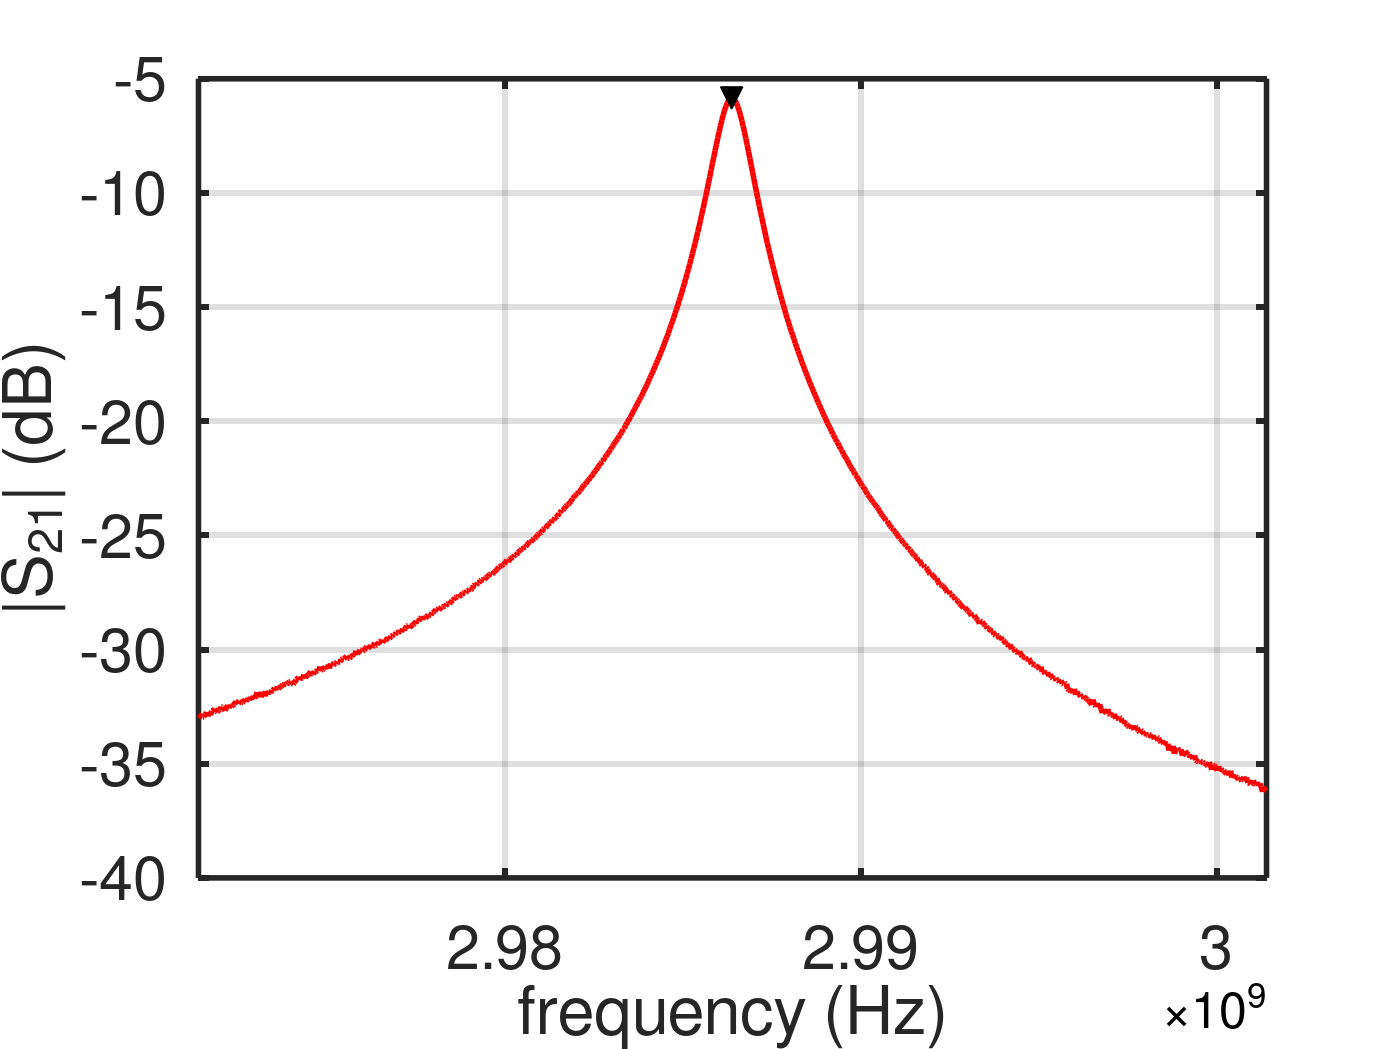
\includegraphics[width=\textwidth]{Images/Relazione6_Foto/fig_1_2_modo4_modulo.png}
\caption{modulo}
\end{subfigure}
\begin{subfigure}{0.49\textwidth}\centering
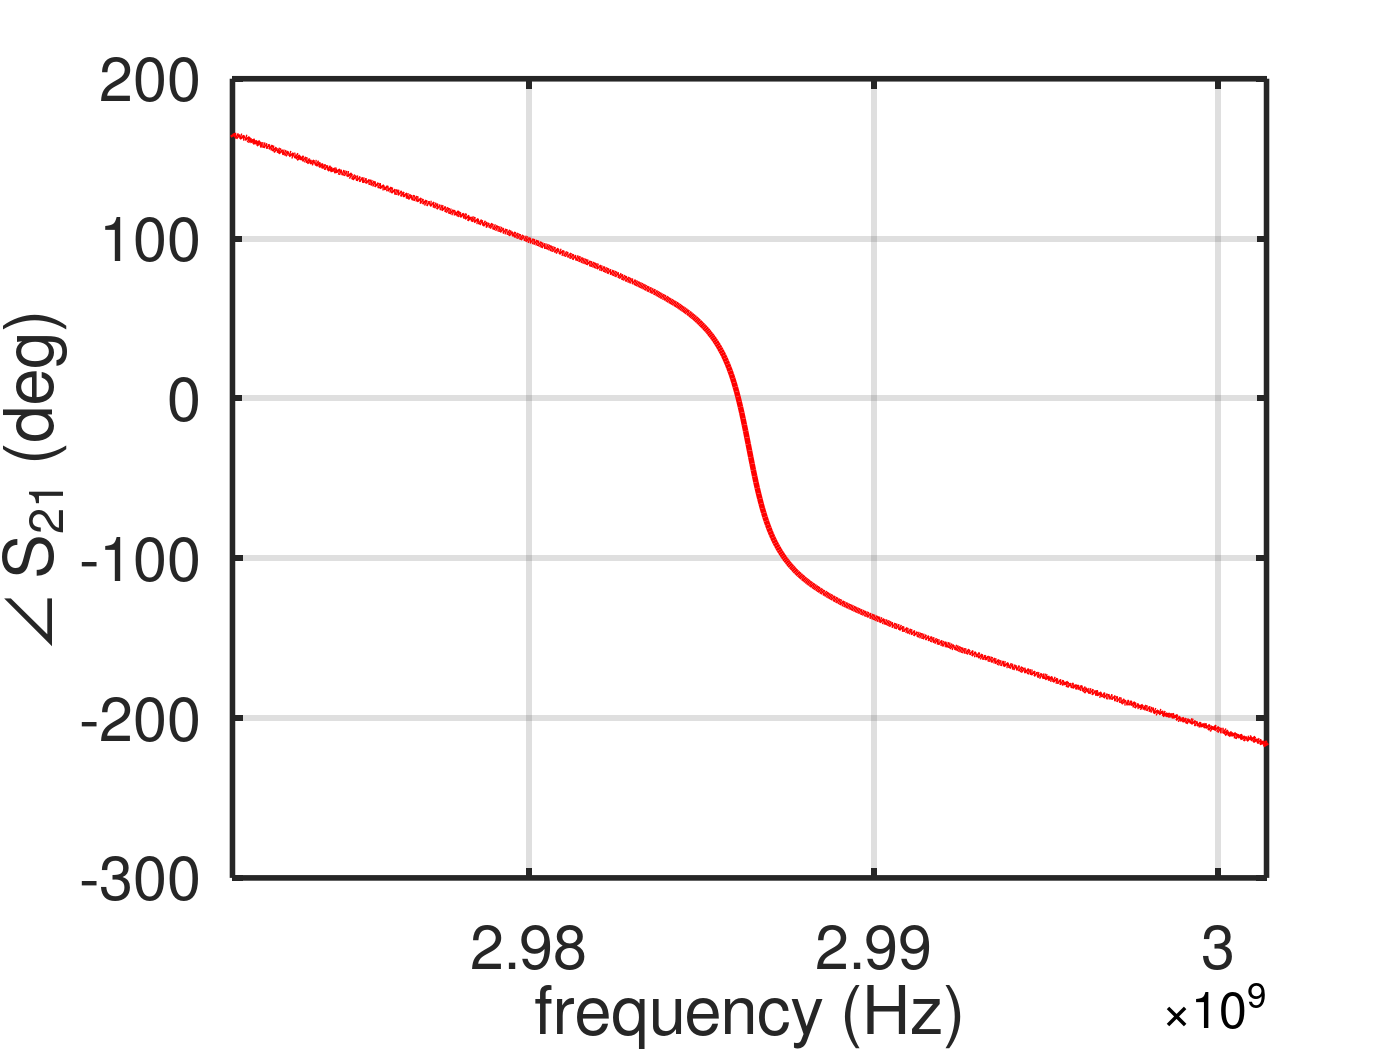
\includegraphics[width=\textwidth]{Images/Relazione6_Foto/fig_1_2_modo4_fase.png}
\caption{fase}
\end{subfigure}
\caption{Modo 4: modulo e fase di $S_{21}$ (span 30\,MHz).}
\label{fig:m4}
\end{figure}

Per il primo modo la fase è stata salvata solo come figura di MATLAB, con uno span di 30\,MHz, e non come file di dati: i dati della fase in figura~\ref{fig:m1} li abbiamo quindi ripresi dal file \texttt{.fig}. Su questo span la parte sinistra della traccia è rumorosa, perché lì $|S_{21}|$ scende fin quasi a $-60$\,dB.

Dalla misura otteniamo i valori in tabella~\ref{tab:modulo}.

\begin{table}[H]
\centering
\renewcommand{\arraystretch}{1.2}
\begin{tabular}{c c c c c c}
\hline
modo & $f_0$ [GHz] & $BW$ [kHz] & $Q_L$ & $\Delta f$ [kHz] & punti nella banda \\ \hline
1 & $1.939663 \pm 0.000002$ & $234.5 \pm 4.1$ & $8271 \pm 144$ & 10 & 23 \\
2 & $1.964197 \pm 0.000008$ & $271 \pm 15$ & $7240 \pm 409$ & 37.5 & 7 \\
3 & $2.858146 \pm 0.000008$ & $674 \pm 15$ & $4241 \pm 96$ & 37.5 & 18 \\
4 & $2.986376 \pm 0.000008$ & $1112 \pm 15$ & $2685 \pm 37$ & 37.5 & 30 \\ \hline
\end{tabular}
\caption{$f_0$, banda a $-3$\,dB e $Q_L$ dei quattro modi, con le incertezze della (\ref{eq:incbanda}).}
\label{tab:modulo}
\end{table}

Il primo modo è stato acquisito su 8\,MHz, con 10\,kHz fra due punti, e nella banda cadono 23 punti. Gli altri tre modi li abbiamo acquisiti su 30\,MHz, con 37.5\,kHz fra due punti: per il secondo modo, che è il più stretto dei tre, nella banda cadono solo 7 punti e l'incertezza su $Q_L$ arriva al 6\%. Per misurarlo meglio avremmo dovuto restringere lo span come per il primo modo. Si nota anche che il fattore di merito scende passando dai modi a 1.9\,GHz a quelli a 2.9\,GHz.

\section{Confronto con la curva teorica (punto 1.3)}
Con $f_0$ e $Q_L$ della tabella~\ref{tab:modulo} calcoliamo la (\ref{eq:S21norm}) e la sovrapponiamo alla misura normalizzata al valore in $f_0$, mettendo $\delta$ sull'asse delle ascisse come chiede la scheda. Di seguito i grafici per i quattro modi:

\begin{figure}[H]
\centering
\begin{subfigure}{0.49\textwidth}\centering
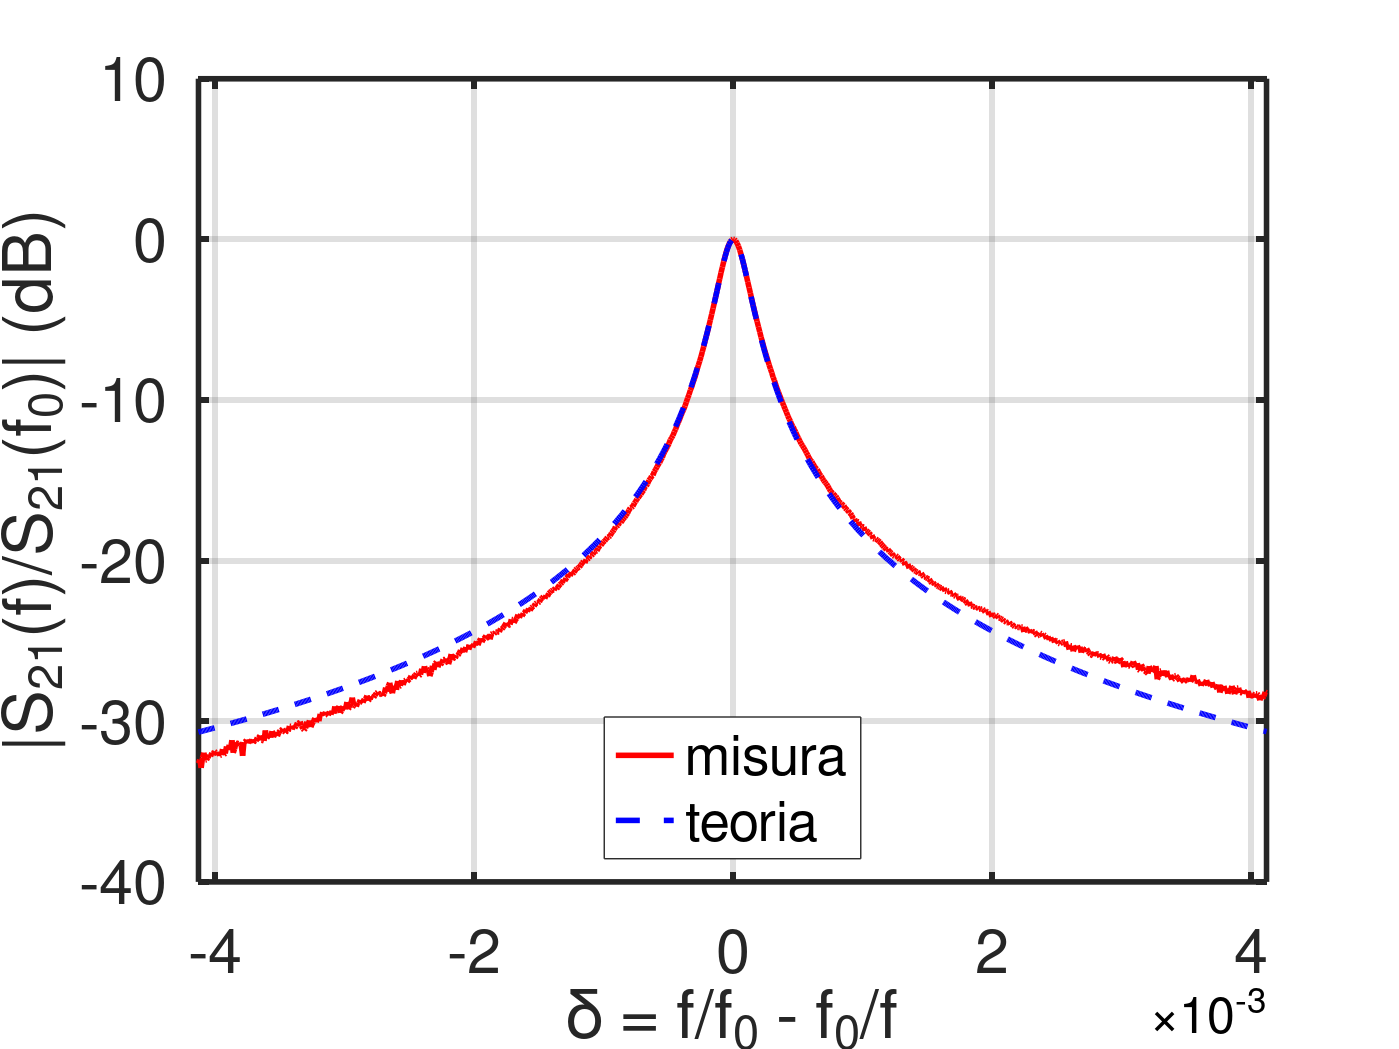
\includegraphics[width=\textwidth]{Images/Relazione6_Foto/fig_1_3_modo1.png}
\caption{modo 1}
\end{subfigure}
\begin{subfigure}{0.49\textwidth}\centering
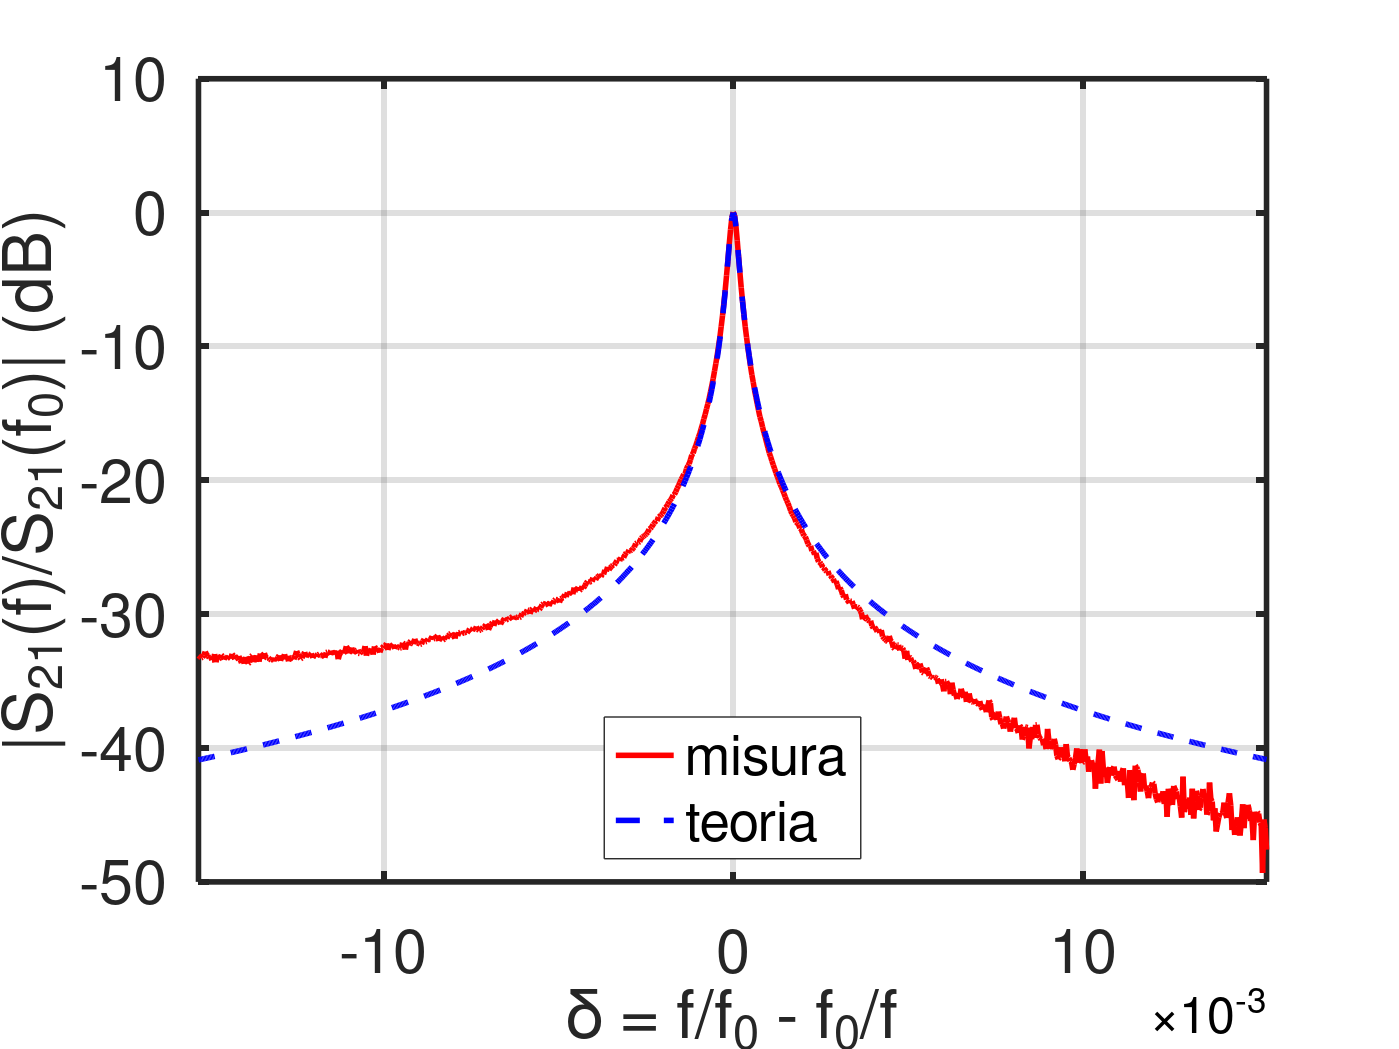
\includegraphics[width=\textwidth]{Images/Relazione6_Foto/fig_1_3_modo2.png}
\caption{modo 2}
\end{subfigure}
\begin{subfigure}{0.49\textwidth}\centering
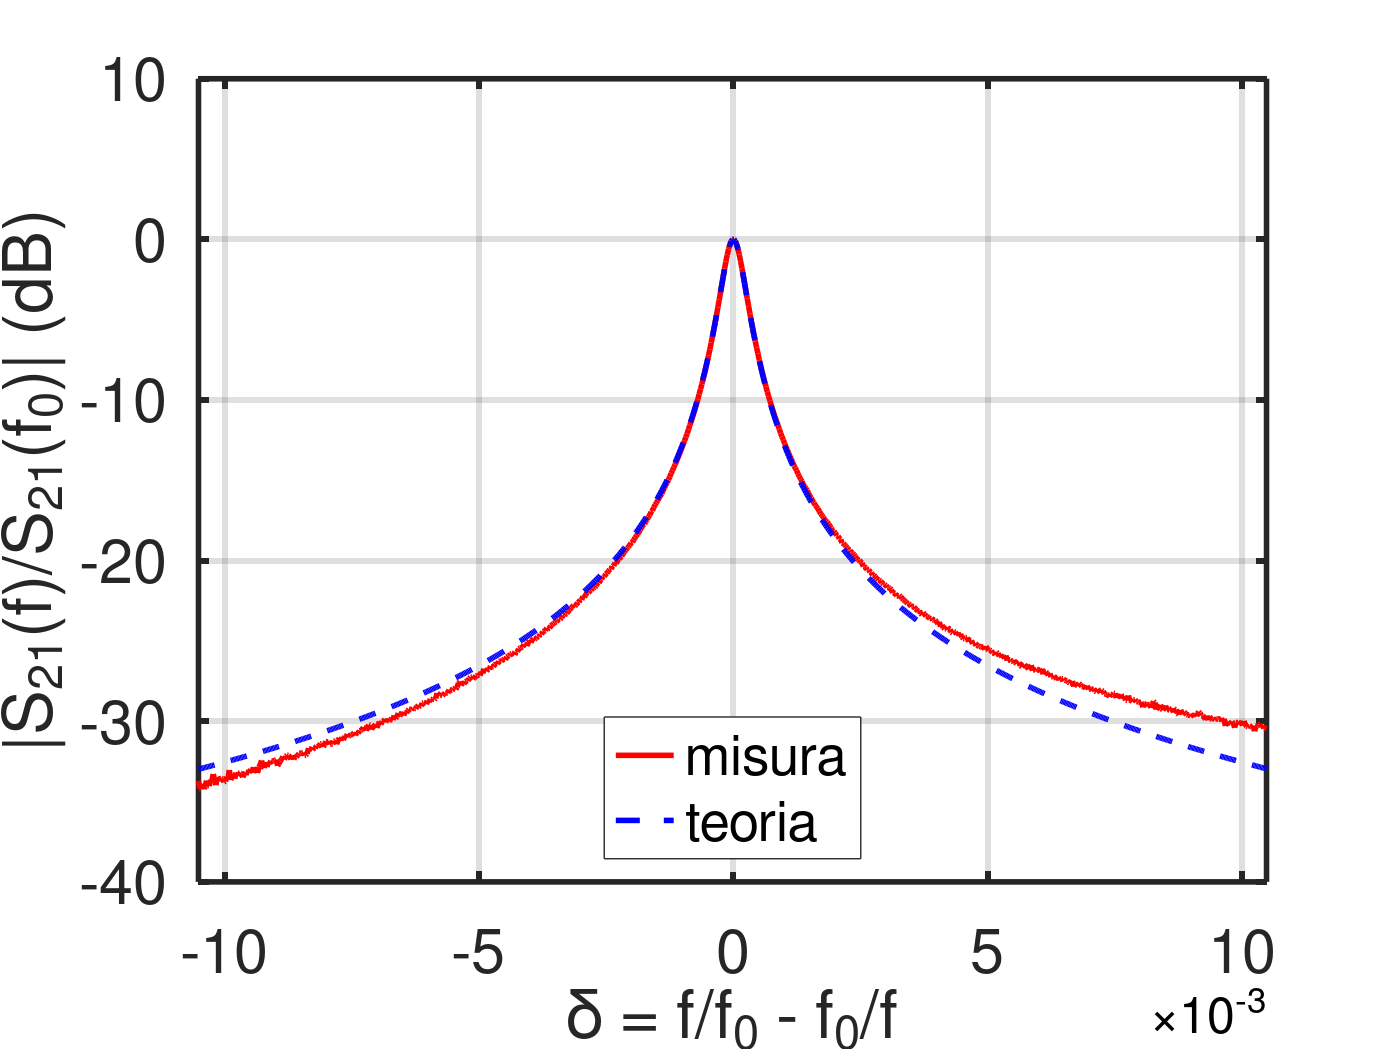
\includegraphics[width=\textwidth]{Images/Relazione6_Foto/fig_1_3_modo3.png}
\caption{modo 3}
\end{subfigure}
\begin{subfigure}{0.49\textwidth}\centering
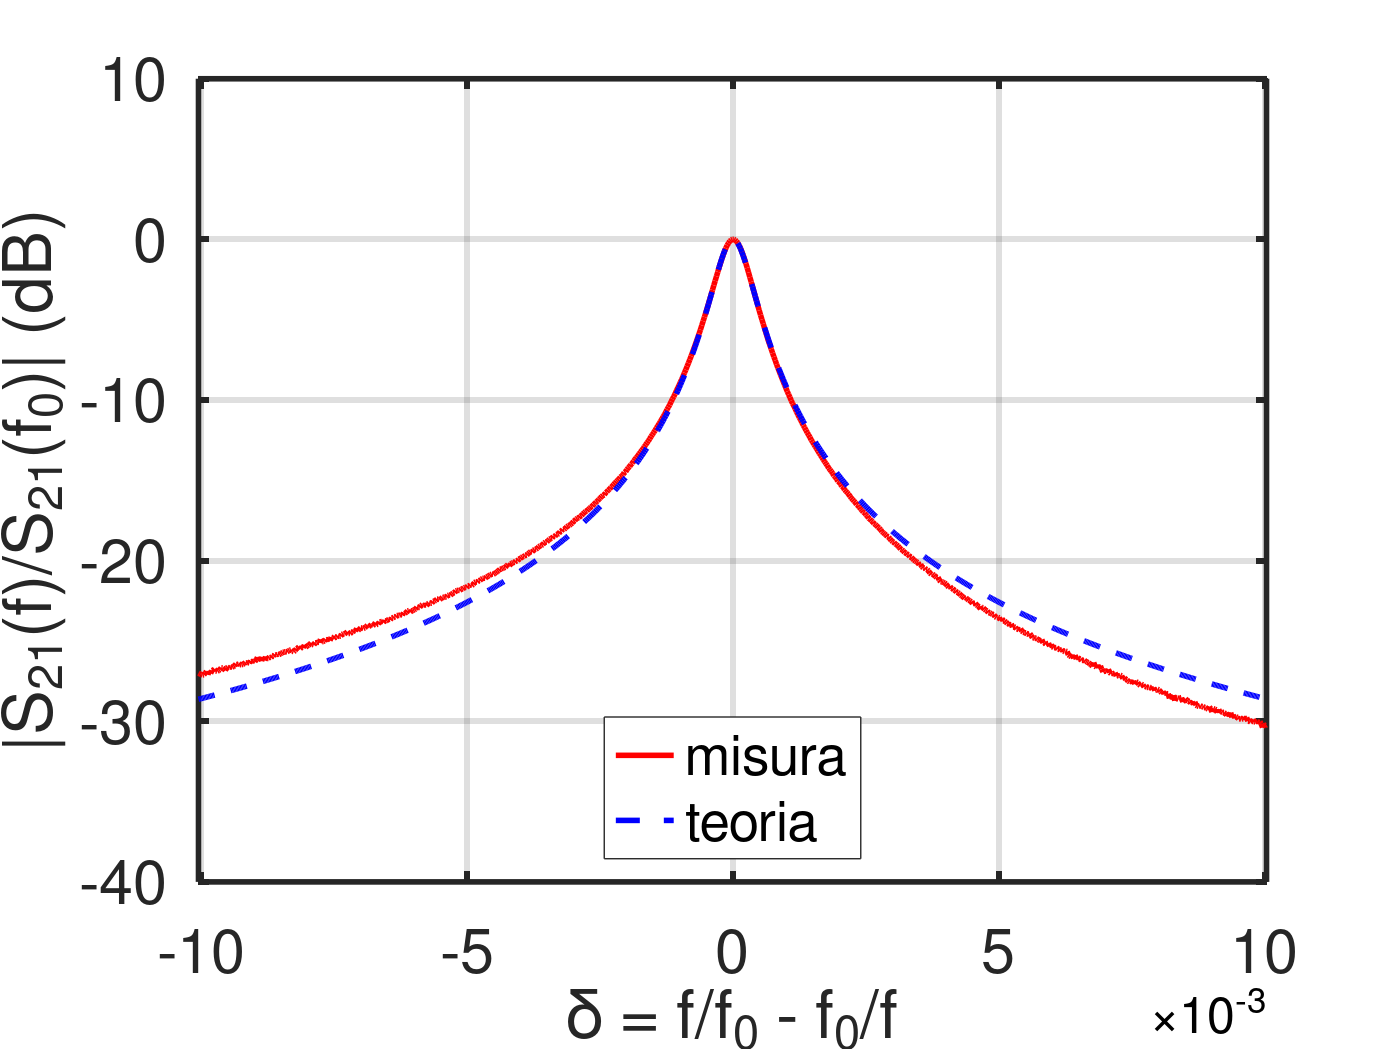
\includegraphics[width=\textwidth]{Images/Relazione6_Foto/fig_1_3_modo4.png}
\caption{modo 4}
\end{subfigure}
\caption{$|S_{21}(f)/S_{21}(f_0)|$ in dB in funzione di $\delta$: misura (rosso) e (\ref{eq:S21norm}) con $f_0$ e $Q_L$ misurati (blu tratteggiato).}
\label{fig:13}
\end{figure}

Come si nota facilmente, vicino alla risonanza misura e teoria coincidono: per $|Q_L\delta|\le1$ lo scarto massimo è di 0.06\,dB per tutti e quattro i modi, e per $|Q_L\delta|\le3$ resta sotto 0.2\,dB. Lontano dalla risonanza, però, la misura si stacca dalla curva. Questo succede perché la (\ref{eq:S21}) descrive un modo isolato, e sulle code della misura si sommano anche le code dei modi vicini e l'accoppiamento diretto fra le due antenne. Infatti la misura sta sopra la curva dalla parte del modo vicino e sotto dall'altra parte, dato che le code dei due modi si sommano con fase diversa ai due lati. Per il modo 1 la coda destra, verso il modo 2, è 2\,dB sopra la teoria; per il modo 2 la coda sinistra, verso il modo 1, è 7\,dB sopra e quella destra 5\,dB sotto. Lo stesso succede per i modi 3 e 4, con scarti fra 1 e 2.5\,dB. L'effetto più forte è sul modo 2, il cui span di 30\,MHz arriva a meno di 10\,MHz dal modo 1.

\chapter{Misura di $Q_L$ dalla fase di $S_{21}$}
\label{cap:fase}

Lo scopo della seguente misurazione, il punto 1.4 della scheda, è ricavare $Q_L$ dalla pendenza della fase di $S_{21}$ attorno alla risonanza tramite un fit lineare, e confrontarlo con il valore ottenuto dal modulo.

\section{Fit lineare della fase}
Utilizzando la routine del corso \texttt{LinearFit.m}, che si basa su \texttt{regression3}, facciamo il fit del dato formattato in \emph{Unwrapped Phase}, cioè della fase in gradi in funzione della frequenza in Hz, su $NN$ punti centrati su $f_0$. Dalla (\ref{eq:faselin}) la pendenza $p$ in gradi/Hz vale $-\frac{180}{\pi}\frac{2Q_L}{f_0}$, quindi otteniamo
\begin{equation}
Q_L=-p\,\frac{\pi}{180}\,\frac{f_0}{2},\qquad \sigma_{Q_L}=\sigma_p\,\frac{\pi}{180}\,\frac{f_0}{2}.
\label{eq:QLfase}
\end{equation}

La scelta di $NN$ è un compromesso, perché la (\ref{eq:faselin}) vale solo per $|Q_L\delta|\ll1$ ma servono abbastanza punti per il fit. Per i modi 3 e 4 abbiamo preso i punti con $|Q_L\delta|\le0.5$, cioè 9 e 15 punti. Per i modi 1 e 2 la fase è stata acquisita su 30\,MHz, con 37.5\,kHz fra due punti, e con $|Q_L\delta|\le0.5$ ci sarebbero stati solo 3 punti: abbiamo quindi allargato la finestra a $|Q_L\delta|\le1$, cioè 7 punti.

Rispetto alla (\ref{eq:faselin}) ci sono due effetti sistematici di cui tenere conto.

Il primo è il ritardo dei cavi. Senza calibrazione la fase misurata è $\angle S_{21}(f)-2\pi f\tau$ più una costante, dove $\tau$ è il ritardo dei cavi, quindi la pendenza misurata contiene un termine in più, $-360\,\tau$ in gradi/Hz, che fa crescere il $Q_L$ ottenuto dalla (\ref{eq:QLfase}) di $\pi f_0\tau$. Il ritardo lo stimiamo dalla fase lontano dalla risonanza, per $|Q_L\delta|\ge4$, dove dopo aver tolto l'arcotangente della (\ref{eq:fase}) resta solo la retta dovuta ai cavi: otteniamo $\tau$ fra 18 e 20\,ns. Il valore è coerente con quello che si vede in riflessione. La fase di $S_{11}$ e di $S_{22}$ fuori risonanza scende con una pendenza che corrisponde a circa 19\,ns, cioè all'andata e al ritorno su un cavo, quindi circa 9.5\,ns per cavo. In trasmissione il segnale attraversa una volta tutti e due i cavi, quindi il ritardo atteso è $9.5+9.5\simeq19$\,ns. Prima del fit abbiamo tolto questa retta dalla fase, che è come impostare l'\emph{electrical delay} sullo strumento.

Il secondo effetto è la linearizzazione. Sui punti della finestra la retta di regressione approssima l'arcotangente, la cui pendenza diminuisce allontanandosi da $f_0$, quindi il fit sottostima $Q_L$, tanto più quanto più larga è la finestra. Il fattore di correzione si calcola facendo lo stesso fit sulla curva teorica $-\arctan(Q_L\delta)$ negli stessi punti: vale 0.836 e 0.867 per i modi 1 e 2, con $|Q_L\delta|\le1$, e 0.954 per i modi 3 e 4, con $|Q_L\delta|\le0.5$.

\section{Risultati}
In tabella~\ref{tab:fase} riportiamo per ogni modo la pendenza del fit con la sua incertezza, il $Q_L$ che si ottiene direttamente dalla (\ref{eq:QLfase}) e quello corretto per i due effetti.

\begin{table}[H]
\centering
\renewcommand{\arraystretch}{1.25}
\small
\begin{tabular}{c c c c c c c}
\hline
modo & $NN$ & $p$ [$10^{-4}\,^\circ$/Hz] & $Q_L$ dalla (\ref{eq:QLfase}) & $\tau$ [ns] & senza ritardo & $Q_L$ (fase) \\ \hline
1 & 7  & $-4.139 \pm 0.120$ & $7005 \pm 202$ & 18.2 & $6894 \pm 202$ & $8251 \pm 242$ \\
2 & 7  & $-3.728 \pm 0.088$ & $6391 \pm 151$ & 20.2 & $6266 \pm 151$ & $7229 \pm 174$ \\
3 & 9  & $-1.680 \pm 0.015$ & $4190 \pm 38$  & 18.0 & $4029 \pm 38$  & $4223 \pm 39$ \\
4 & 15 & $-1.050 \pm 0.006$ & $2737 \pm 15$  & 19.1 & $2558 \pm 15$  & $2682 \pm 16$ \\ \hline
\end{tabular}
\caption{Fit lineare della fase di $S_{21}$. L'ultima colonna è il $Q_L$ corretto per il ritardo dei cavi e per la linearizzazione; le incertezze sono quelle statistiche del fit.}
\label{tab:fase}
\end{table}

Nella figura~\ref{fig:14} sono sovrapposte, in funzione di $\delta$, la fase misurata relativa a quella in $f_0$, in grigio così come è stata misurata e in rosso dopo aver tolto il ritardo dei cavi, la retta del fit nella finestra usata e la (\ref{eq:fase}) calcolata con $f_0$ e $Q_L$ misurati dal modulo nel capitolo~\ref{cap:modulo}.

\begin{figure}[H]
\centering
\begin{subfigure}{0.49\textwidth}\centering
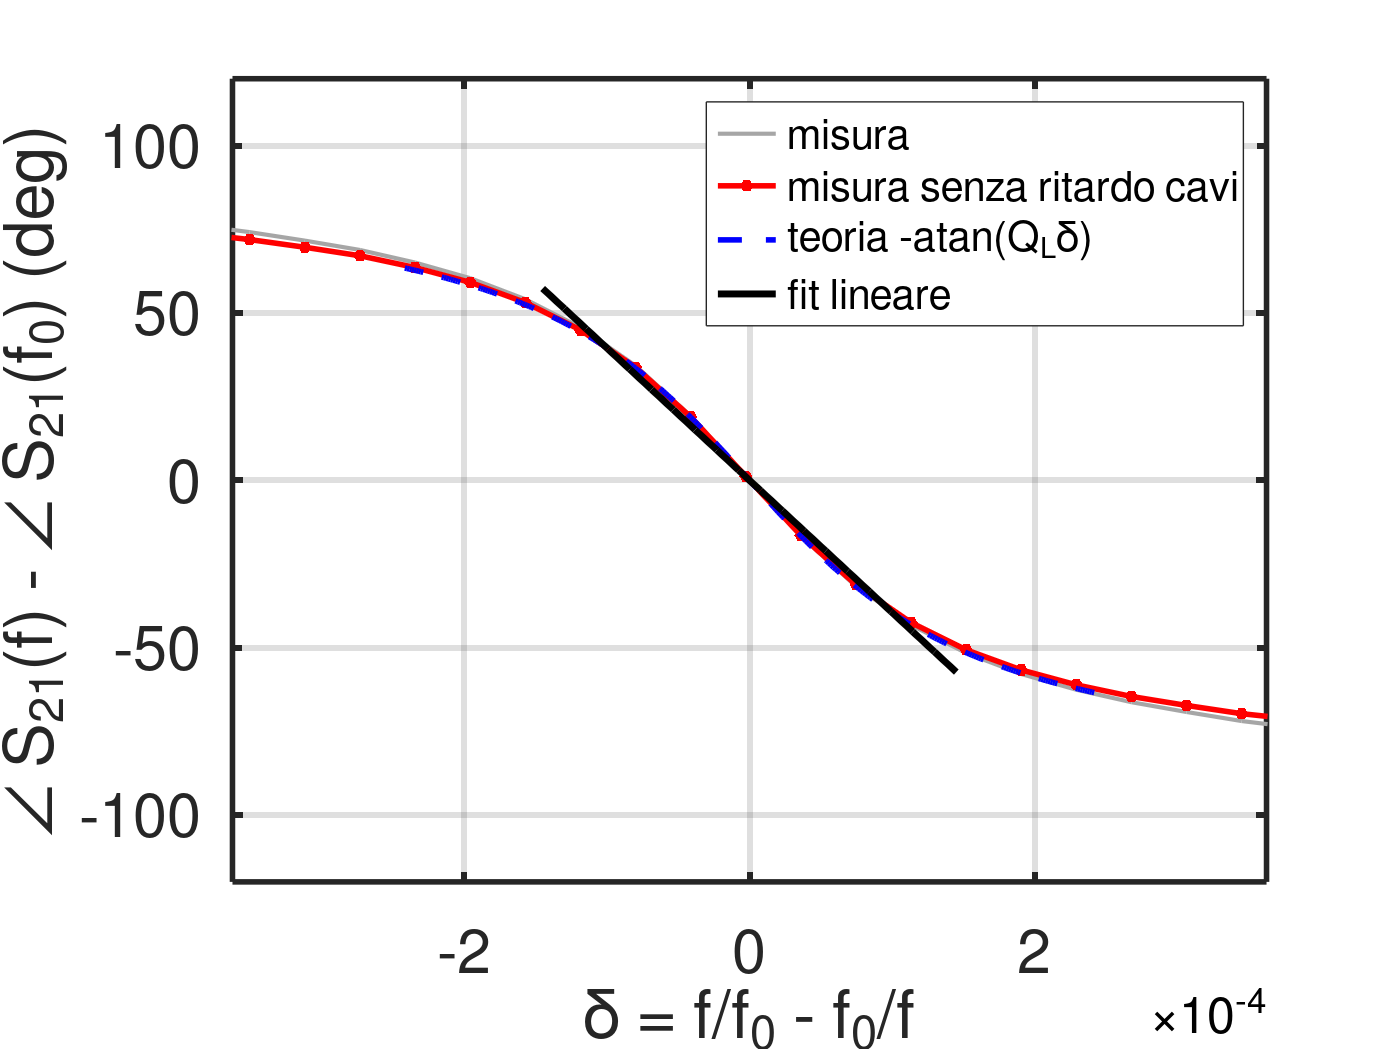
\includegraphics[width=\textwidth]{Images/Relazione6_Foto/fig_1_4_modo1.png}
\caption{modo 1}
\end{subfigure}
\begin{subfigure}{0.49\textwidth}\centering
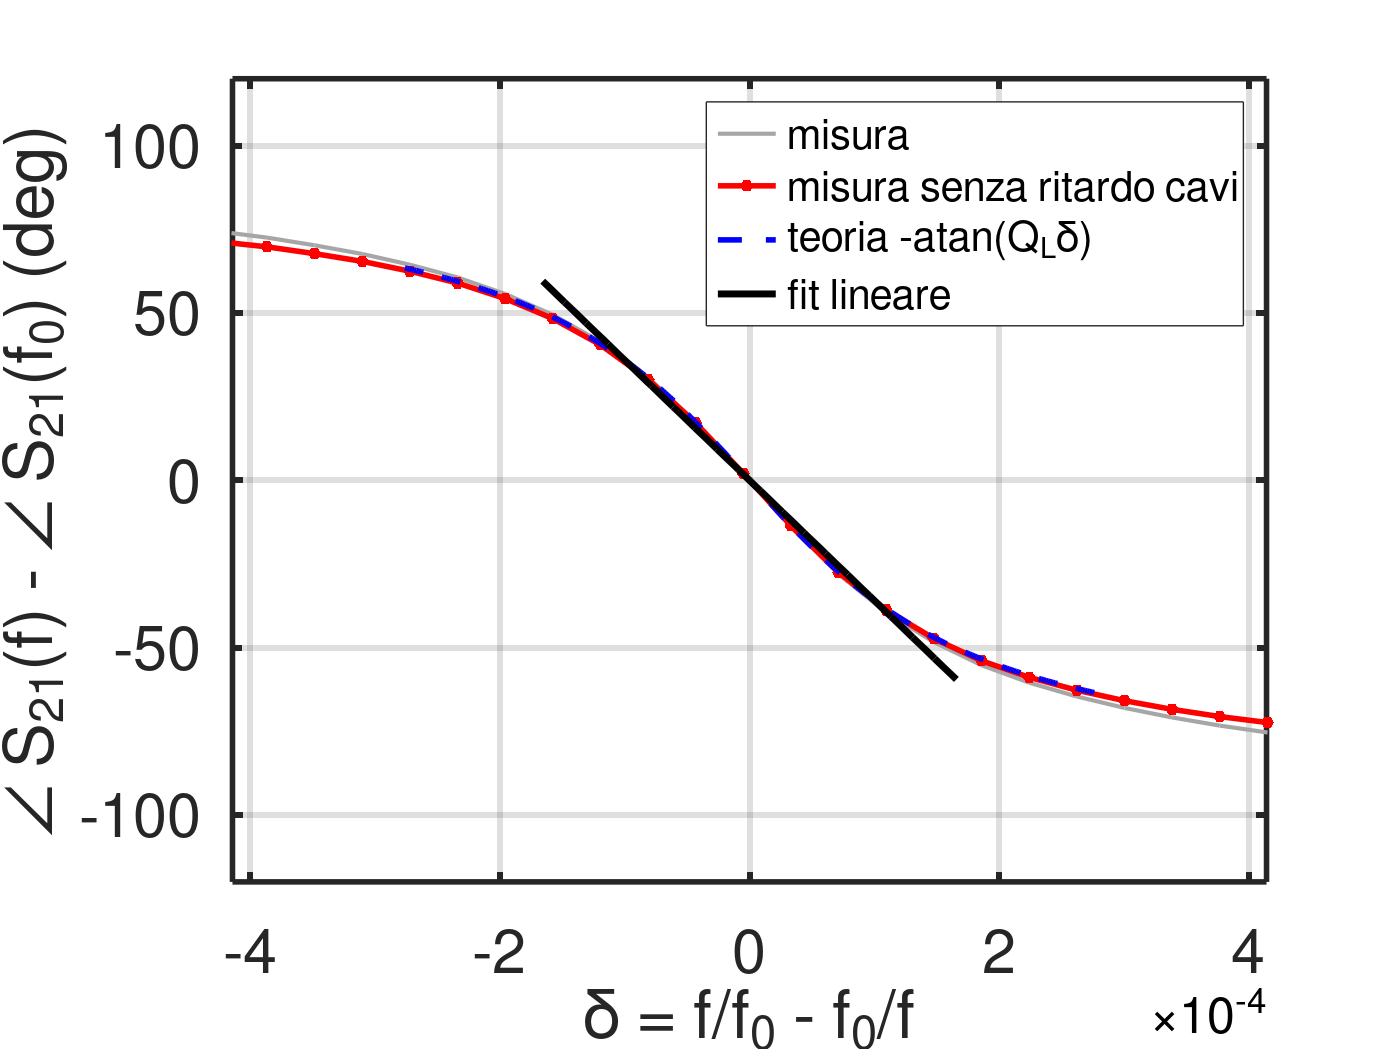
\includegraphics[width=\textwidth]{Images/Relazione6_Foto/fig_1_4_modo2.png}
\caption{modo 2}
\end{subfigure}
\begin{subfigure}{0.49\textwidth}\centering
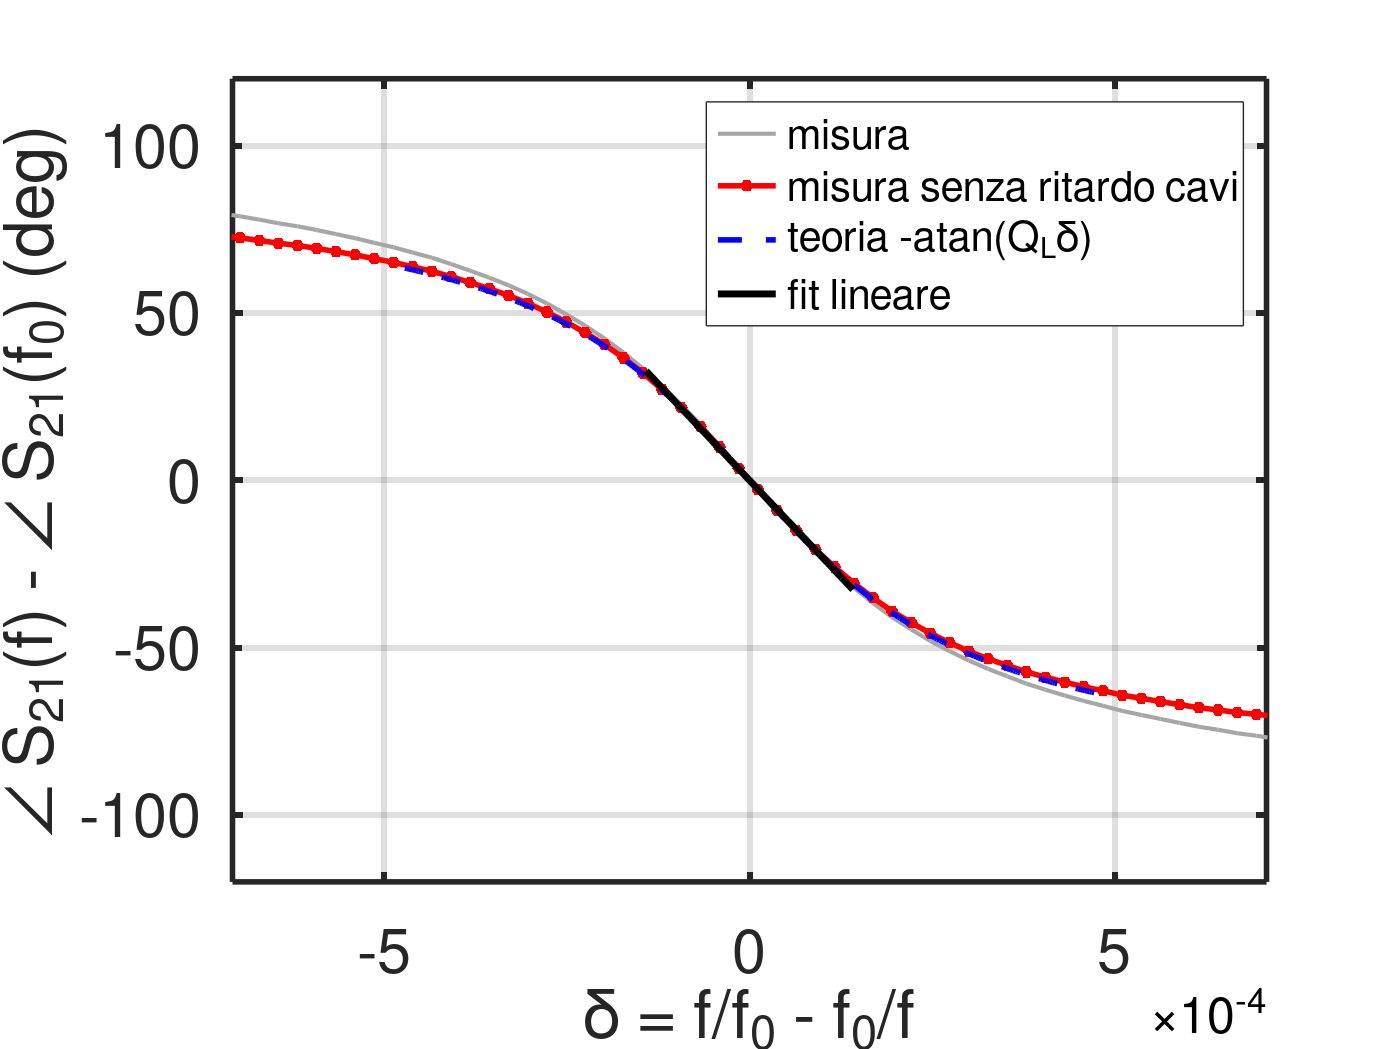
\includegraphics[width=\textwidth]{Images/Relazione6_Foto/fig_1_4_modo3.png}
\caption{modo 3}
\end{subfigure}
\begin{subfigure}{0.49\textwidth}\centering
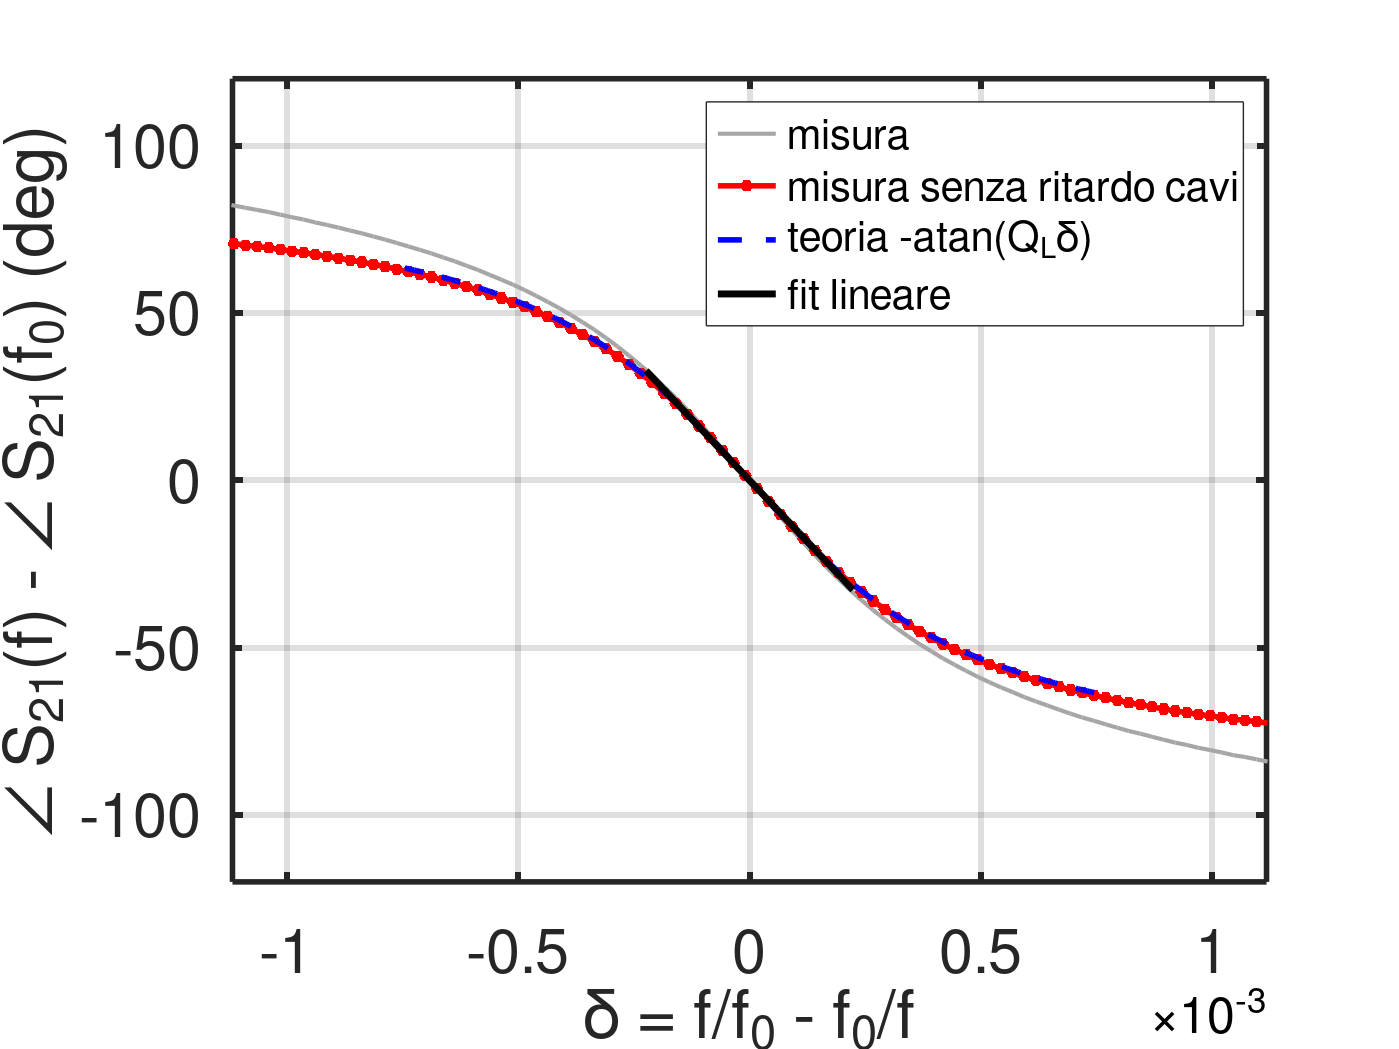
\includegraphics[width=\textwidth]{Images/Relazione6_Foto/fig_1_4_modo4.png}
\caption{modo 4}
\end{subfigure}
\caption{$\angle S_{21}(f)-\angle S_{21}(f_0)$ in funzione di $\delta$: misura, misura senza il ritardo dei cavi, fit lineare e teoria $-\arctan(Q_L\delta)$ con il $Q_L$ del modulo.}
\label{fig:14}
\end{figure}

Come si vede dai grafici, tolto il ritardo dei cavi la fase misurata si sovrappone alla curva teorica su tutto l'intervallo, anche dove la fase non è più lineare. La misura grezza invece si allontana sempre di più dalla teoria man mano che ci si allontana da $f_0$. Dopo le due correzioni il $Q_L$ dalla fase differisce da quello del modulo di $-0.2$\%, $-0.1$\%, $-0.4$\% e $-0.1$\% per i quattro modi, sempre entro l'incertezza. Senza correzioni gli scarti sarebbero stati molto più grandi: per i modi 1 e 2 il fit su $|Q_L\delta|\le1$ dà un $Q_L$ più basso del 12--15\%, e per i modi 3 e 4 il ritardo dei cavi da solo fa crescere $Q_L$ di 160--180, cioè del 4--7\%. L'incertezza della tabella è solo quella statistica del fit e non tiene conto degli errori sistematici. Per i modi 1 e 2 sarebbe stato meglio acquisire la fase con uno span più stretto, in modo da avere più punti con $|Q_L\delta|\le0.25$, dove la linearizzazione introduce un errore di circa l'1\%.

\chapter{Coefficienti di accoppiamento e $Q_0$}
\label{cap:beta}

In questo capitolo ricaviamo i coefficienti di accoppiamento $\beta_1$ e $\beta_2$ dalle misure di $S_{11}$ e $S_{22}$ e da questi il fattore di merito a vuoto $Q_0$, come chiede il punto 1.5. Poi passiamo a confrontare $|S_{21}(\delta)|$ misurato con la (\ref{eq:S21}) calcolata con tutti i parametri misurati, come chiede il punto 1.6.

\section{Formule usate}
Dalla teoria sappiamo che alla risonanza la cavità, vista da una porta con l'altra porta chiusa sui 50\,$\Omega$ dello strumento, è equivalente a una resistenza. Per un modo sottoaccoppiato il coefficiente di riflessione alle due porte vale
\begin{equation}
\Delta S_{11}=\frac{1+\beta_2-\beta_1}{1+\beta_1+\beta_2},\qquad
\Delta S_{22}=\frac{1+\beta_1-\beta_2}{1+\beta_1+\beta_2},
\label{eq:deltaS}
\end{equation}
dove $\Delta S_{11}$ e $\Delta S_{22}$ sono i valori di $|S_{11}|$ e $|S_{22}|$ alla risonanza, in lineare, rispetto al valore fuori risonanza. Invertendo si ottengono le formule del corso:
\begin{equation}
\beta_1=\frac{1-\Delta S_{11}}{\Delta S_{11}+\Delta S_{22}},\qquad
\beta_2=\frac{1-\Delta S_{22}}{\Delta S_{11}+\Delta S_{22}},\qquad
Q_0=Q_L(1+\beta_1+\beta_2)=\frac{2Q_L}{\Delta S_{11}+\Delta S_{22}}.
\label{eq:beta}
\end{equation}
Prendere la buca rispetto al livello fuori risonanza è importante nel nostro caso, poiché le misure non sono calibrate: il cavo attenua allo stesso modo dentro e fuori risonanza e nel rapporto la sua attenuazione si semplifica. Le formule valgono solo se tutte e due le antenne sono sottoaccoppiate, e questo lo abbiamo verificato con la carta di Smith.

Come ci è stato indicato in laboratorio, il punto 1.5 lo abbiamo fatto solo per i due modi più bassi, quindi abbiamo acquisito $S_{11}$ e $S_{22}$ solo per i modi 1 e 2. Per i modi 3 e 4 il punto 1.6 è fatto normalizzando al massimo, come chiede la scheda per i modi a cui le formule non si applicano.

\section{Modo 1}
In figura~\ref{fig:15m1} sono riportati $|S_{11}|$ e $|S_{22}|$ attorno al primo modo e in figura~\ref{fig:smith1} $S_{11}$ sulla carta di Smith.

\begin{figure}[H]
\centering
\begin{subfigure}{0.49\textwidth}\centering
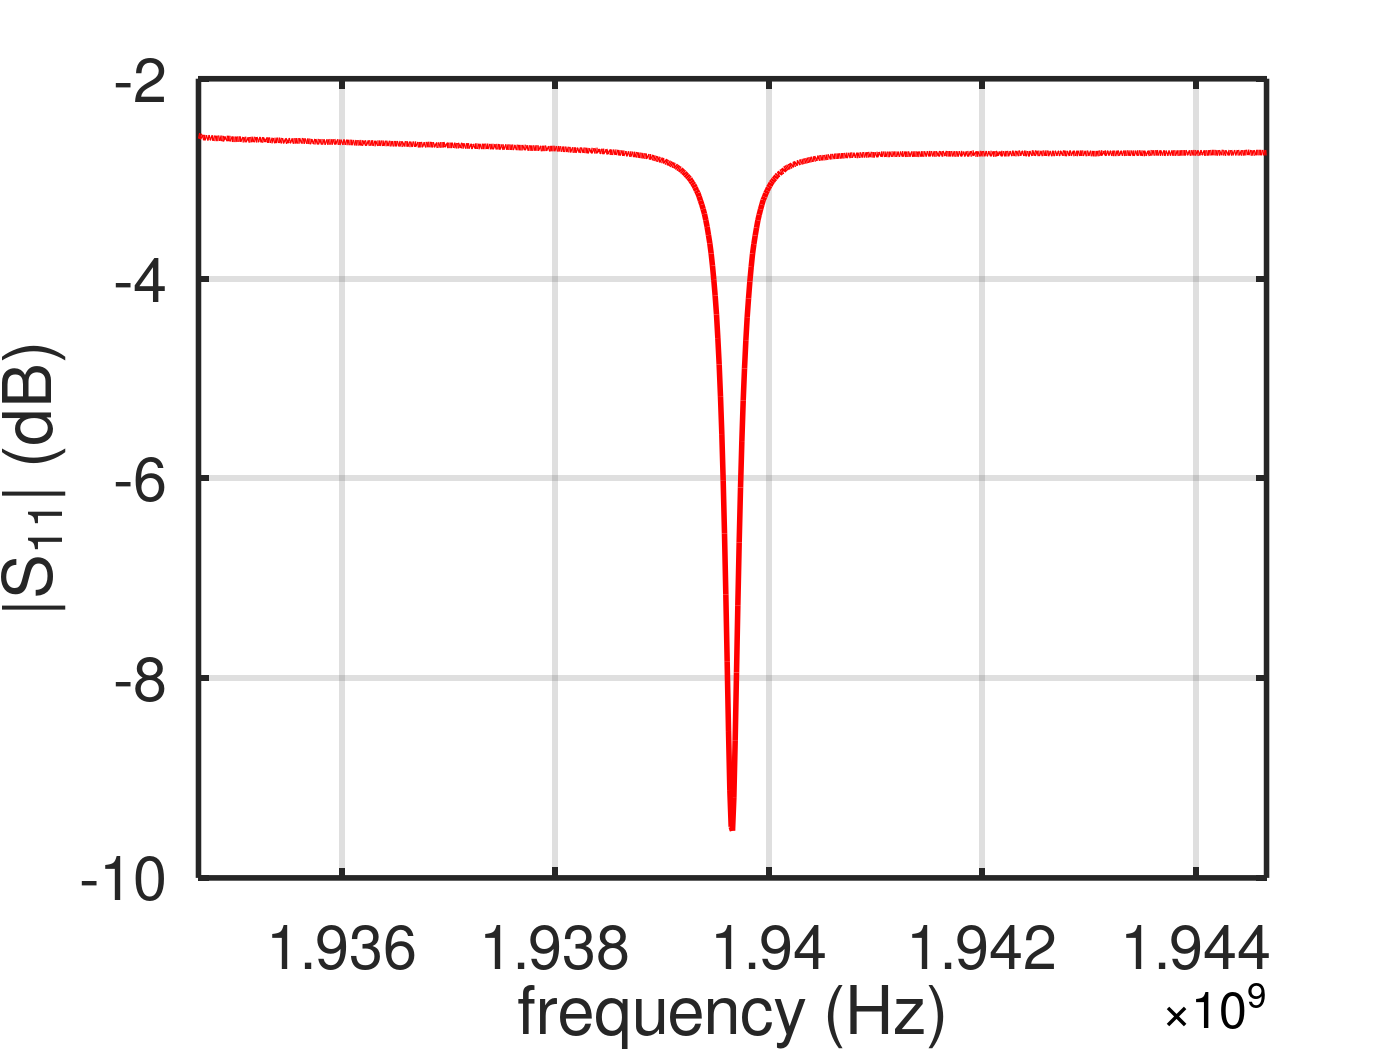
\includegraphics[width=\textwidth]{Images/Relazione6_Foto/fig_1_5_modo1_S11.png}
\caption{$|S_{11}|$}
\end{subfigure}
\begin{subfigure}{0.49\textwidth}\centering
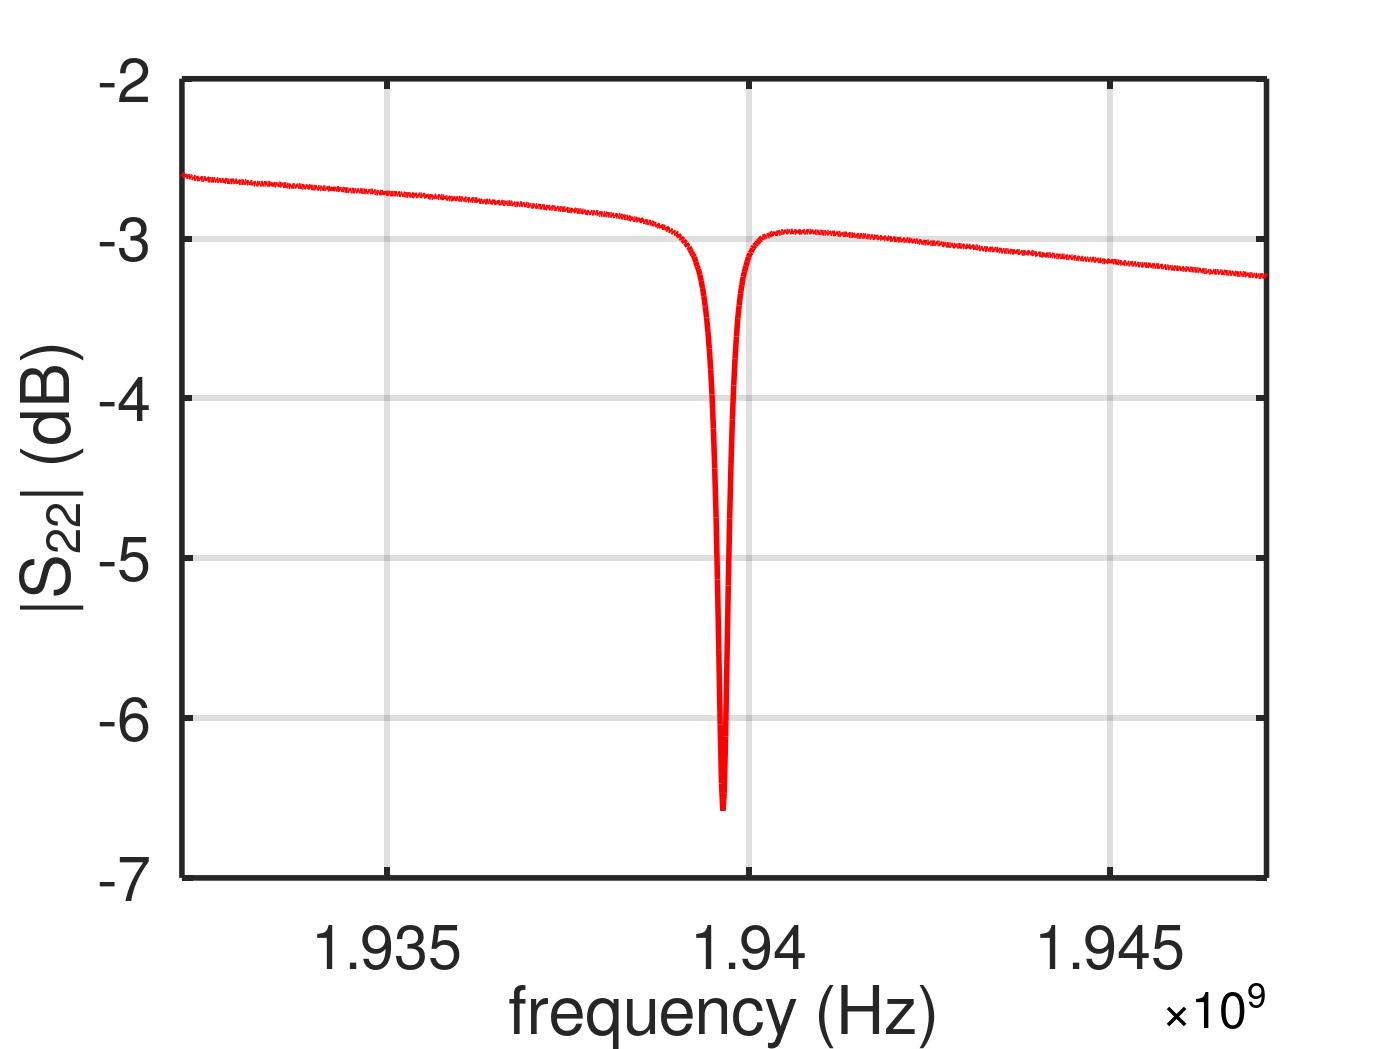
\includegraphics[width=\textwidth]{Images/Relazione6_Foto/fig_1_5_modo1_S22.png}
\caption{$|S_{22}|$}
\end{subfigure}
\caption{Modo 1: modulo di $S_{11}$ (span 10\,MHz) e di $S_{22}$ (span 15\,MHz).}
\label{fig:15m1}
\end{figure}

\begin{figure}[H]
\centering
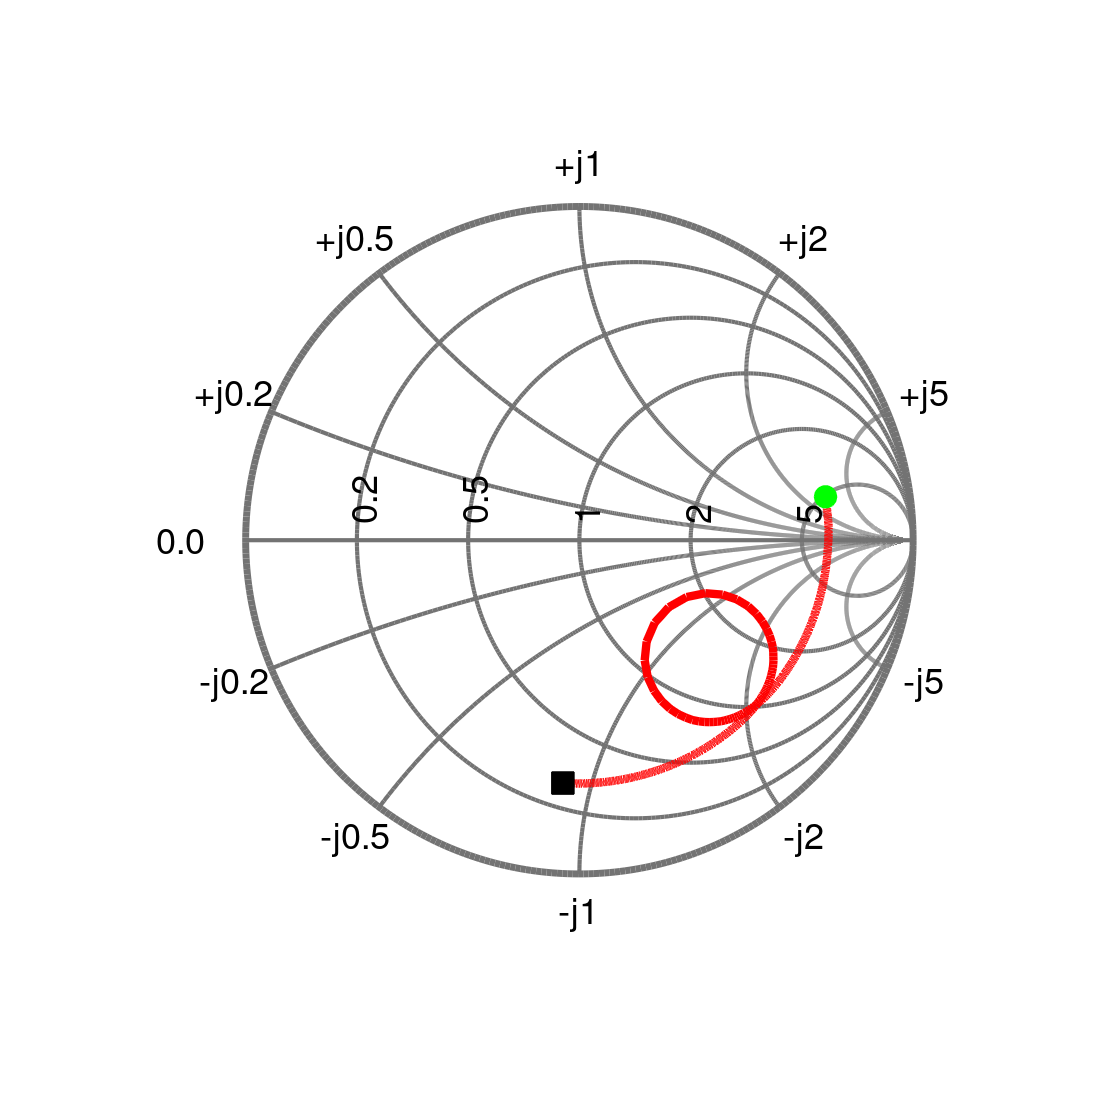
\includegraphics[width=0.5\textwidth]{Images/Relazione6_Foto/fig_1_5_modo1_smith.png}
\caption{Modo 1: $S_{11}$ sulla carta di Smith, dal punto verde (1.932\,GHz) al quadrato nero (1.947\,GHz).}
\label{fig:smith1}
\end{figure}

Sulla carta di Smith la risonanza è il piccolo cerchio, che non contiene il centro della carta: l'antenna 1 è quindi sottoaccoppiata. Il resto della traccia è un arco di raggio circa 0.73, che corrisponde al livello di $-2.7$\,dB fuori risonanza, percorso in senso orario al crescere della frequenza a causa del ritardo del cavo. Rispetto alla misura calibrata il cerchio è più piccolo e ruotato, ma scalare e ruotare la traccia attorno al centro della carta non cambia il fatto che il cerchio contenga o no il centro, quindi la verifica vale anche senza calibrazione. Per $S_{22}$ non abbiamo salvato la carta di Smith, però lo stesso controllo si può fare sui dati complessi del file: tolta la pendenza dovuta al cavo, attraversando la risonanza la fase di $S_{22}$ non compie un giro completo, quindi anche il suo cerchio non contiene il centro e anche l'antenna 2 è sottoaccoppiata.

Il livello fuori risonanza è stato preso come mediana dei punti alle due estremità della traccia, cioè il primo e l'ultimo 10\%. Per $S_{11}$ otteniamo $-2.682$\,dB fuori risonanza e un minimo di $-9.528$\,dB a 1.939660\,GHz, quindi una buca di 6.846\,dB. Per $S_{22}$ otteniamo $-2.923$\,dB fuori risonanza e un minimo di $-6.580$\,dB, quindi una buca di 3.657\,dB. In lineare
\begin{equation}
\Delta S_{11}=10^{-6.846/20}=0.4547,\qquad \Delta S_{22}=10^{-3.657/20}=0.6563,
\end{equation}
e dalla (\ref{eq:beta})
\begin{equation}
\beta_1=0.491\pm0.004,\qquad \beta_2=0.309\pm0.005,\qquad Q_0=8271\cdot1.800=14888\pm266 .
\end{equation}
Per le incertezze abbiamo considerato $\pm0.05$\,dB sulla profondità di ciascuna buca, poiché il livello di riferimento è la parte più incerta della misurazione: la traccia di $S_{22}$ fuori risonanza non è piatta e scende di circa 0.6\,dB da un estremo all'altro. L'incertezza su $Q_0$ è dominata da quella di $Q_L$.

\section{Modo 2}
Passiamo ora al secondo modo, le cui misure sono nelle figure~\ref{fig:15m2} e~\ref{fig:smith2}.

\begin{figure}[H]
\centering
\begin{subfigure}{0.49\textwidth}\centering
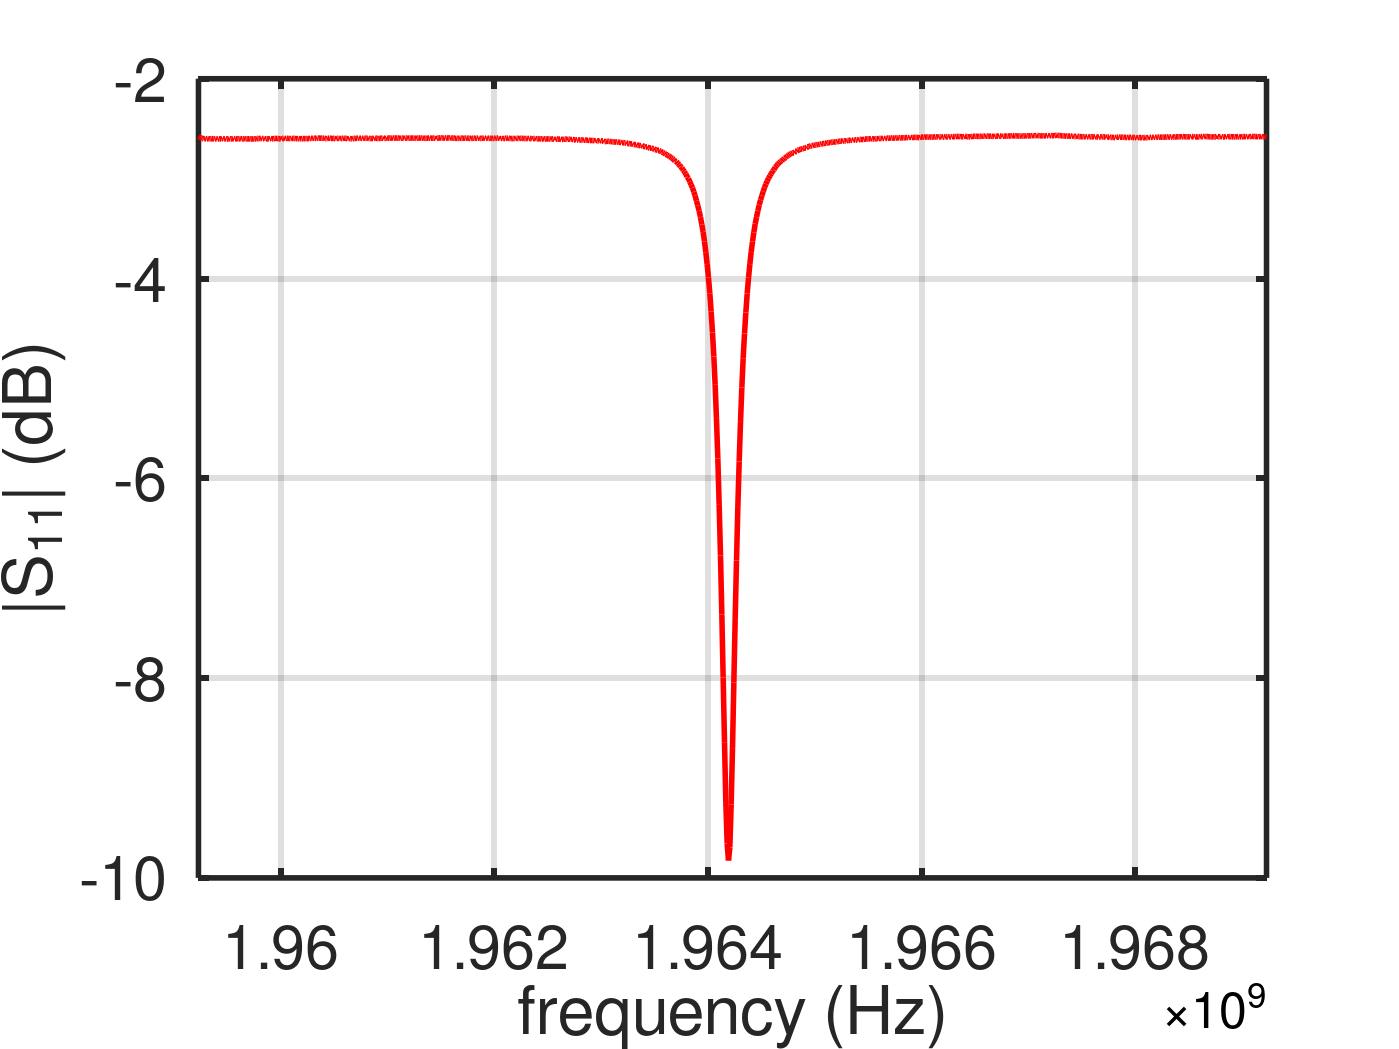
\includegraphics[width=\textwidth]{Images/Relazione6_Foto/fig_1_5_modo2_S11.png}
\caption{$|S_{11}|$}
\end{subfigure}
\begin{subfigure}{0.49\textwidth}\centering
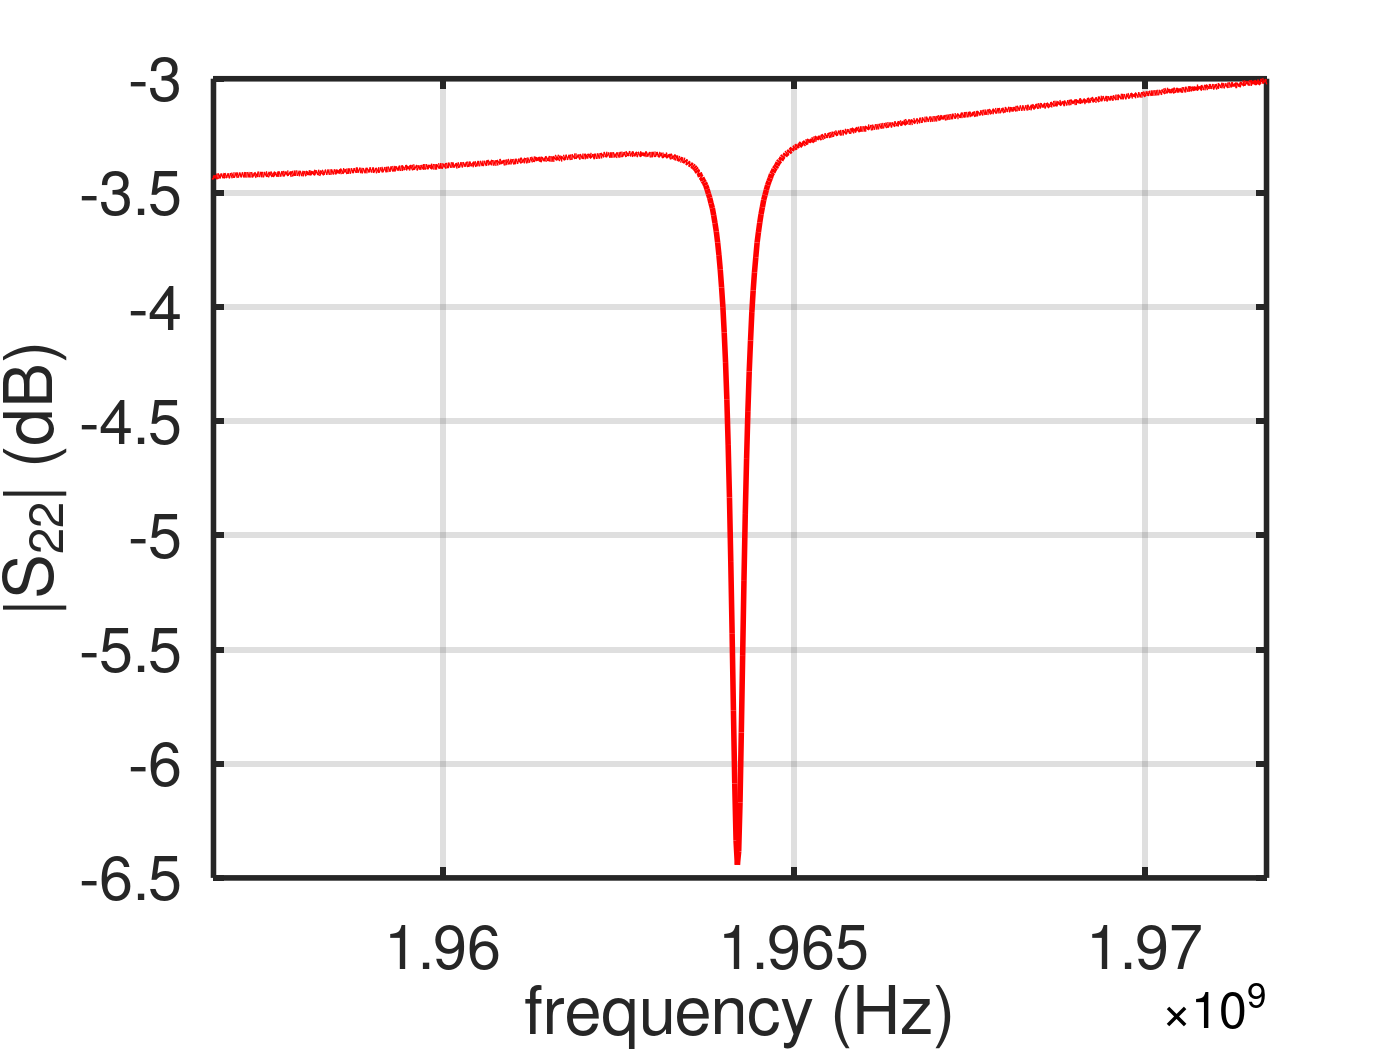
\includegraphics[width=\textwidth]{Images/Relazione6_Foto/fig_1_5_modo2_S22.png}
\caption{$|S_{22}|$}
\end{subfigure}
\caption{Modo 2: modulo di $S_{11}$ (span 10\,MHz) e di $S_{22}$ (span 15\,MHz).}
\label{fig:15m2}
\end{figure}

\begin{figure}[H]
\centering
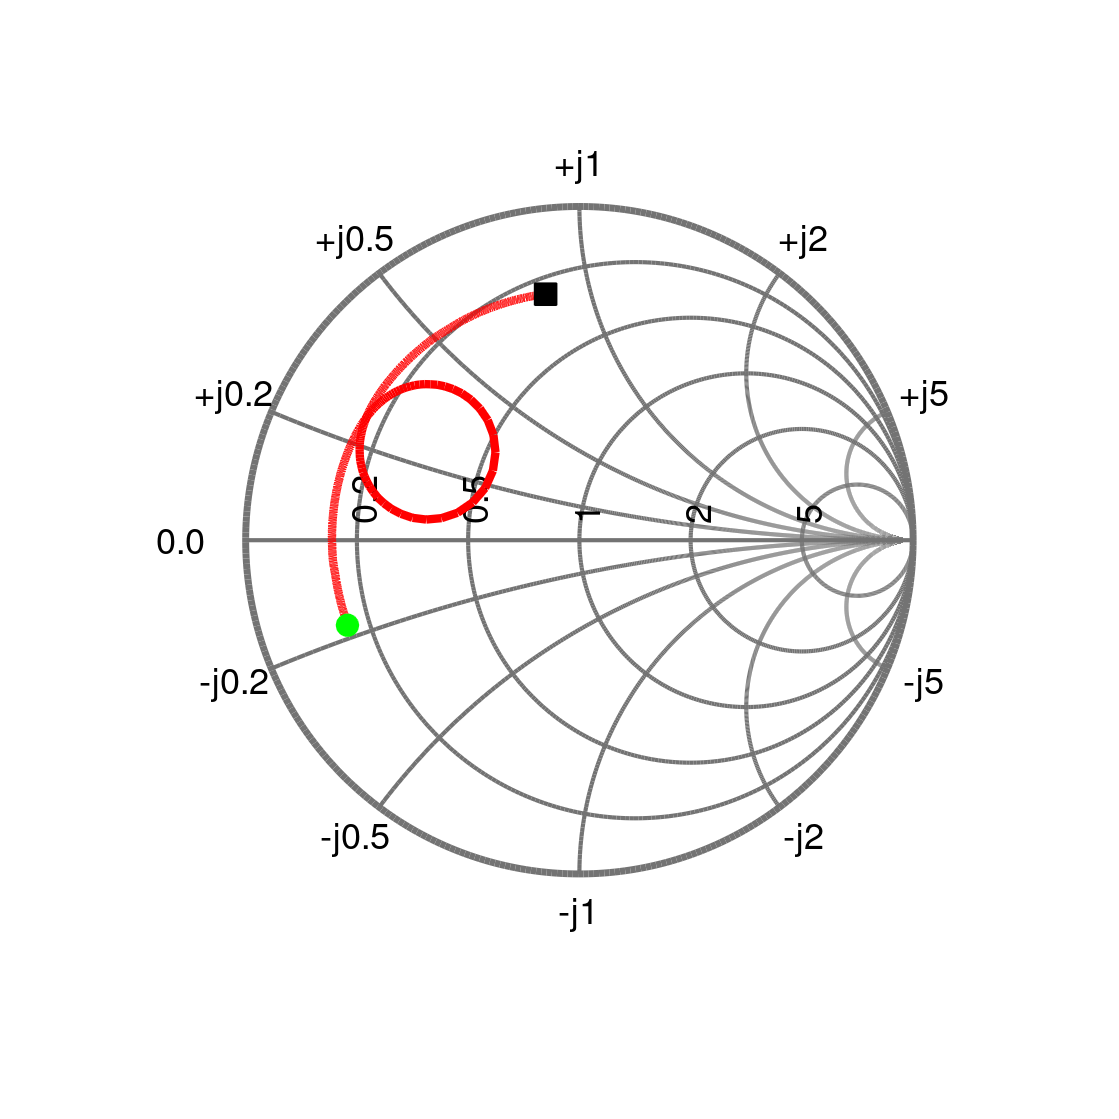
\includegraphics[width=0.5\textwidth]{Images/Relazione6_Foto/fig_1_5_modo2_smith.png}
\caption{Modo 2: $S_{11}$ sulla carta di Smith, dal punto verde (1.957\,GHz) al quadrato nero (1.972\,GHz).}
\label{fig:smith2}
\end{figure}

Anche in questo caso il cerchio della risonanza non contiene il centro della carta e il controllo sulla fase di $S_{22}$ dà lo stesso risultato, quindi entrambe le antenne sono sottoaccoppiate. Per $S_{11}$ il livello fuori risonanza è $-2.586$\,dB e il minimo $-9.826$\,dB a 1.964193\,GHz, con una buca di 7.241\,dB; per $S_{22}$ il livello fuori risonanza è $-3.234$\,dB e il minimo $-6.443$\,dB, con una buca di 3.208\,dB. Otteniamo quindi
\begin{equation}
\Delta S_{11}=0.4345,\qquad \Delta S_{22}=0.6912,
\end{equation}
\begin{equation}
\beta_1=0.502\pm0.004,\qquad \beta_2=0.274\pm0.005,\qquad Q_0=7240\cdot1.777=12863\pm728 .
\end{equation}
L'incertezza su $Q_0$ è più grande che per il modo 1 perché lo è quella su $Q_L$, dato che nella banda cadono pochi punti. Si nota anche che in tutti e due i modi l'antenna 1 è accoppiata più dell'antenna 2.

\section{$|S_{21}(\delta)|$ misurato e teorico (punto 1.6)}
Con $f_0$, $Q_L$, $\beta_1$ e $\beta_2$ misurati calcoliamo $|S_{21}(\delta)|$ in dB dalle (\ref{eq:S21}) e (\ref{eq:S21f0}) e lo sovrapponiamo alla misura in figura~\ref{fig:16}. Per i modi 3 e 4 la misura e la curva sono normalizzate al massimo.

\begin{figure}[H]
\centering
\begin{subfigure}{0.49\textwidth}\centering
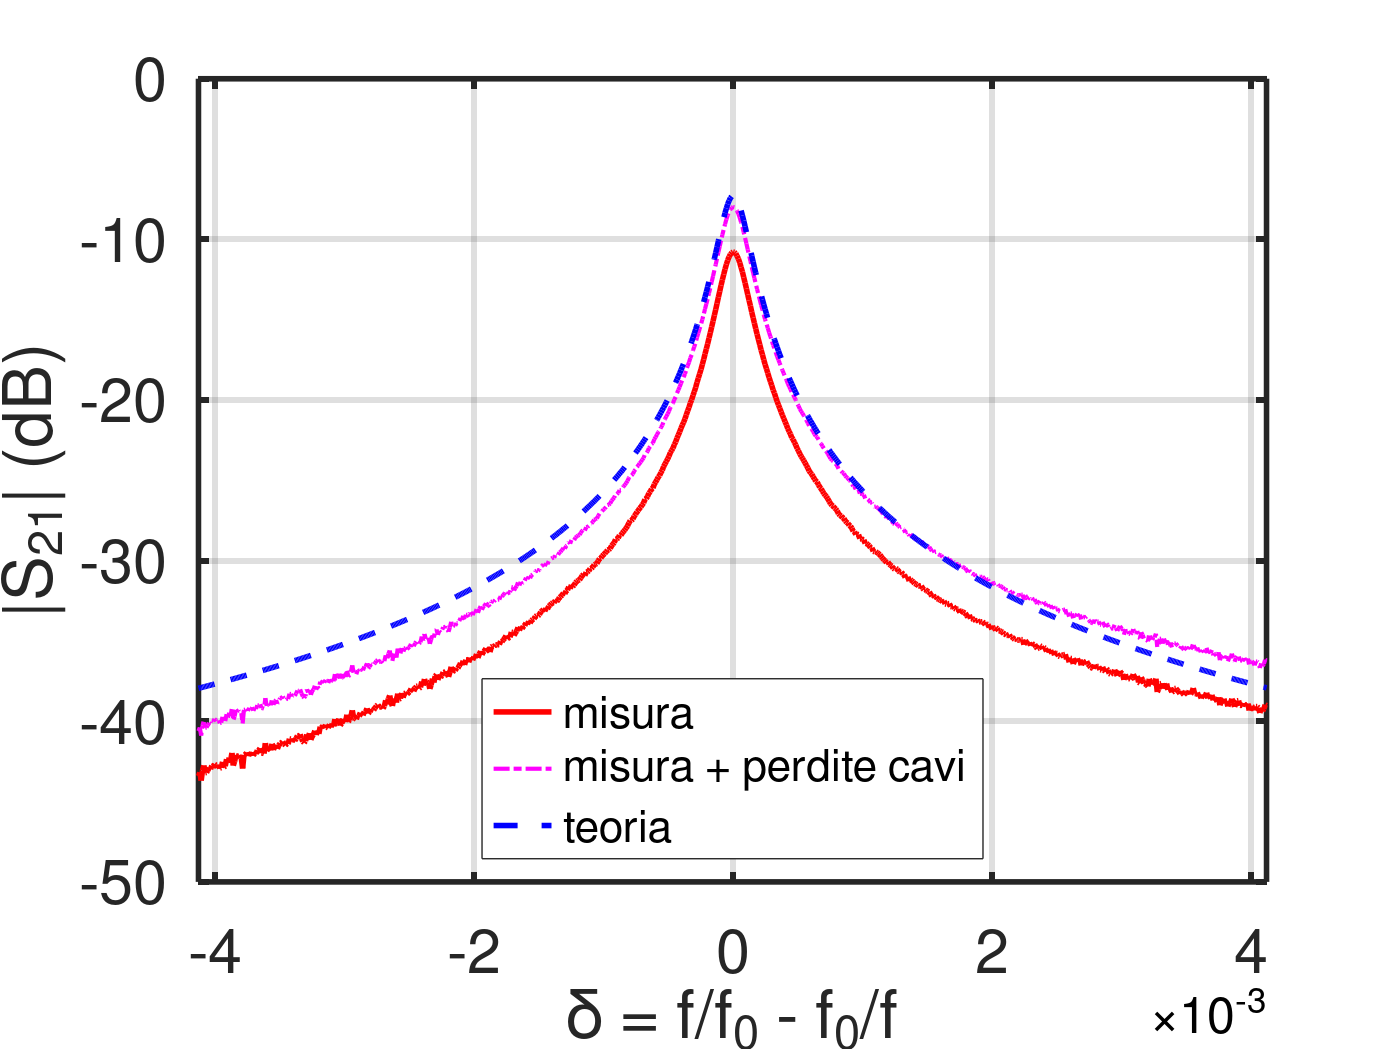
\includegraphics[width=\textwidth]{Images/Relazione6_Foto/fig_1_6_modo1.png}
\caption{modo 1}
\end{subfigure}
\begin{subfigure}{0.49\textwidth}\centering
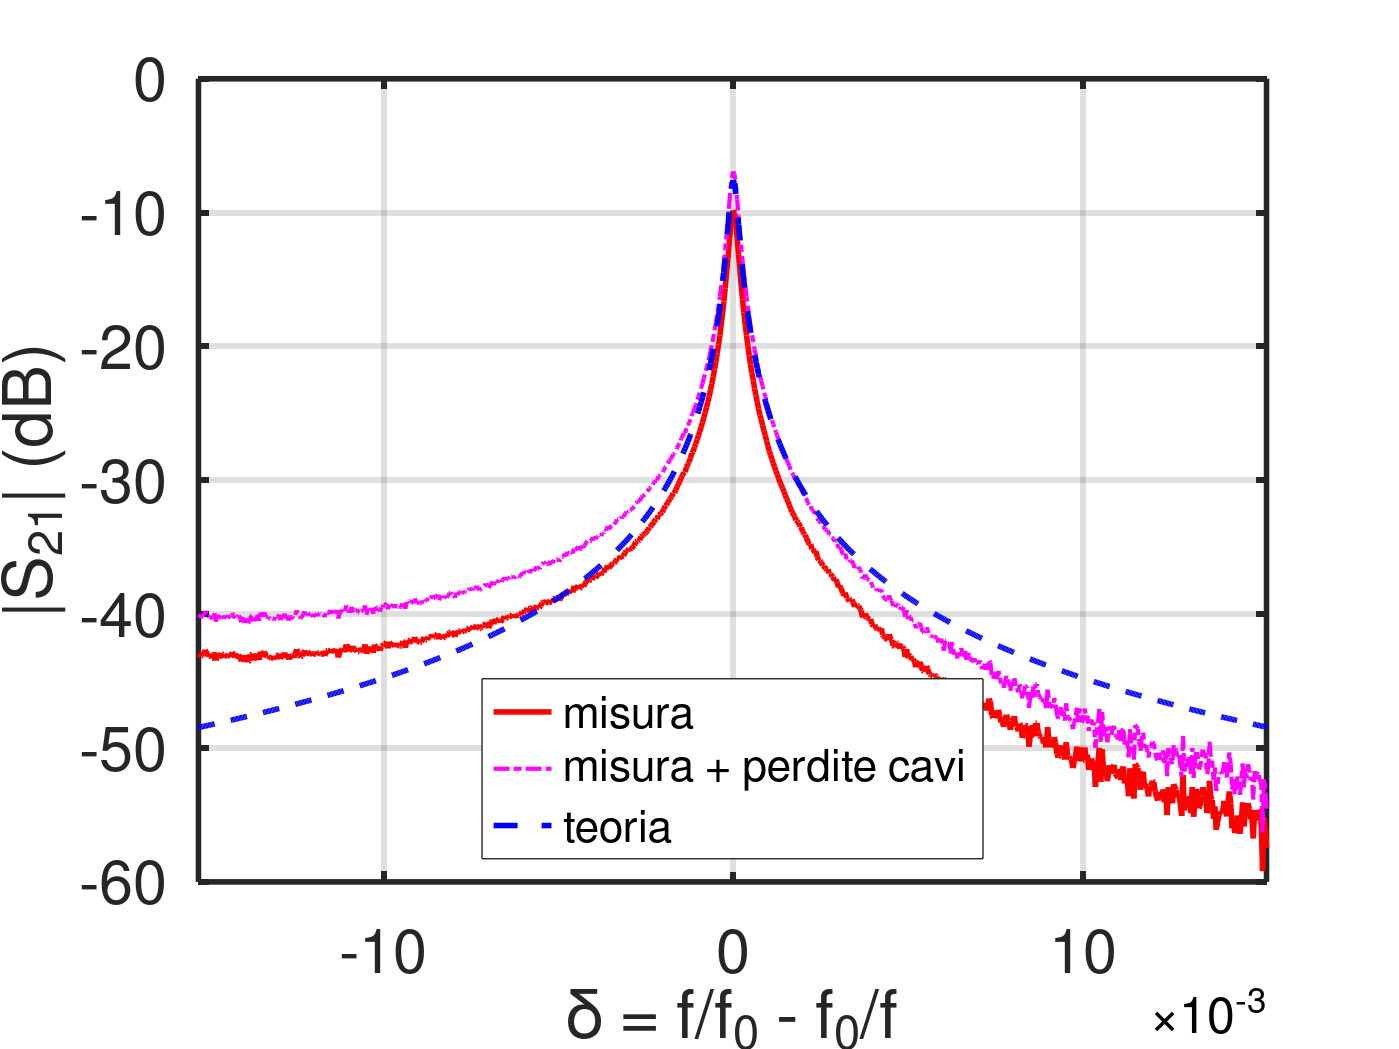
\includegraphics[width=\textwidth]{Images/Relazione6_Foto/fig_1_6_modo2.png}
\caption{modo 2}
\end{subfigure}
\begin{subfigure}{0.49\textwidth}\centering
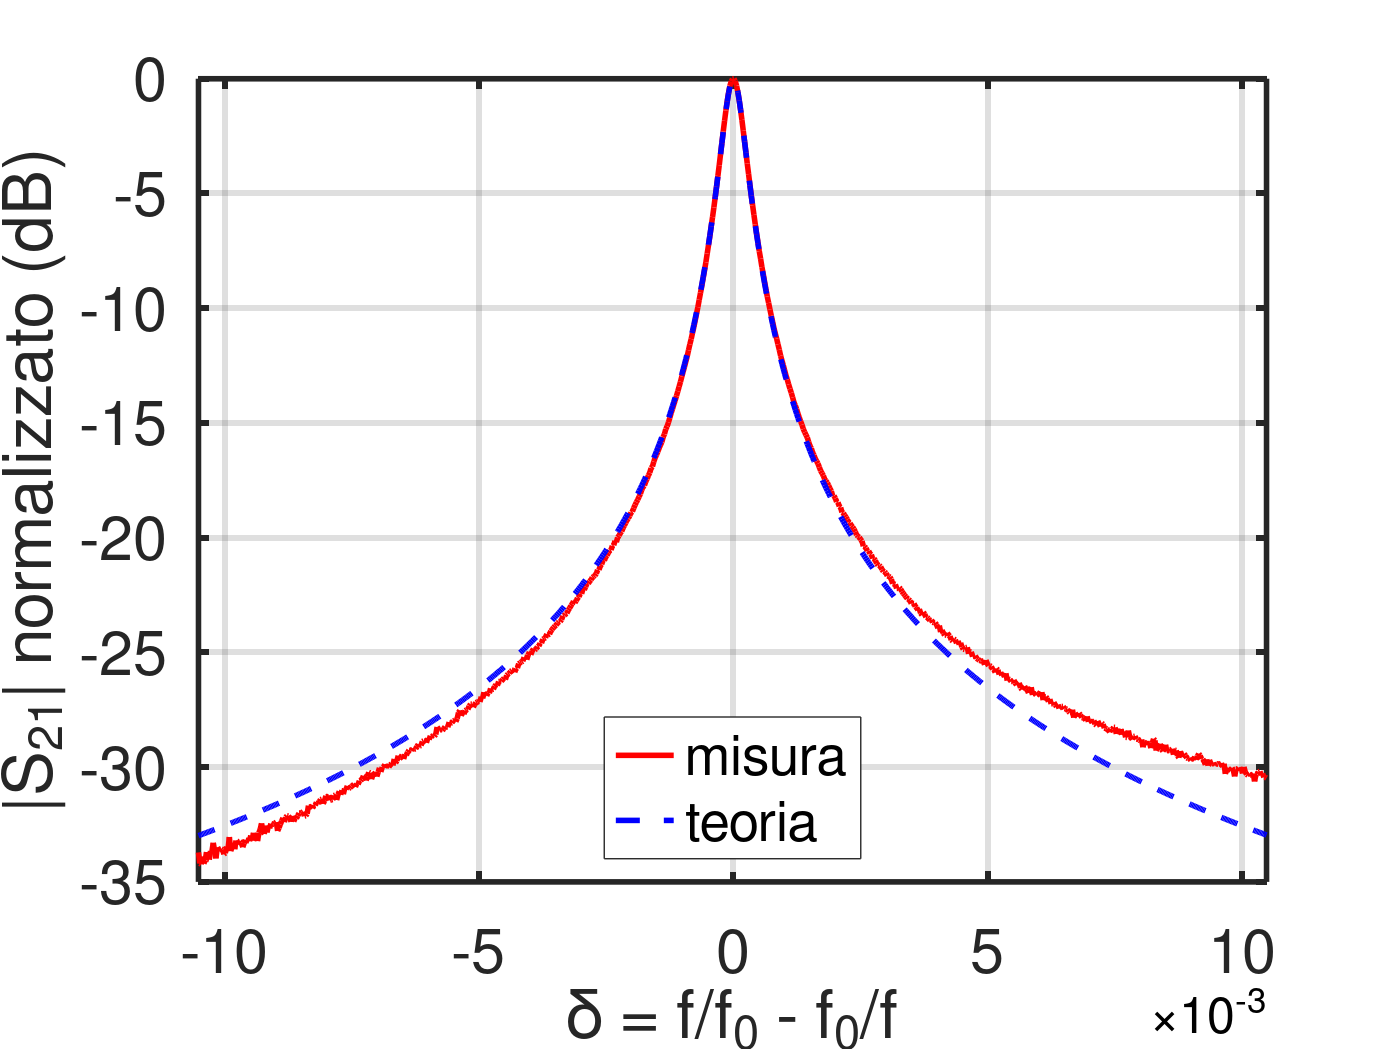
\includegraphics[width=\textwidth]{Images/Relazione6_Foto/fig_1_6_modo3.png}
\caption{modo 3 (normalizzato)}
\end{subfigure}
\begin{subfigure}{0.49\textwidth}\centering
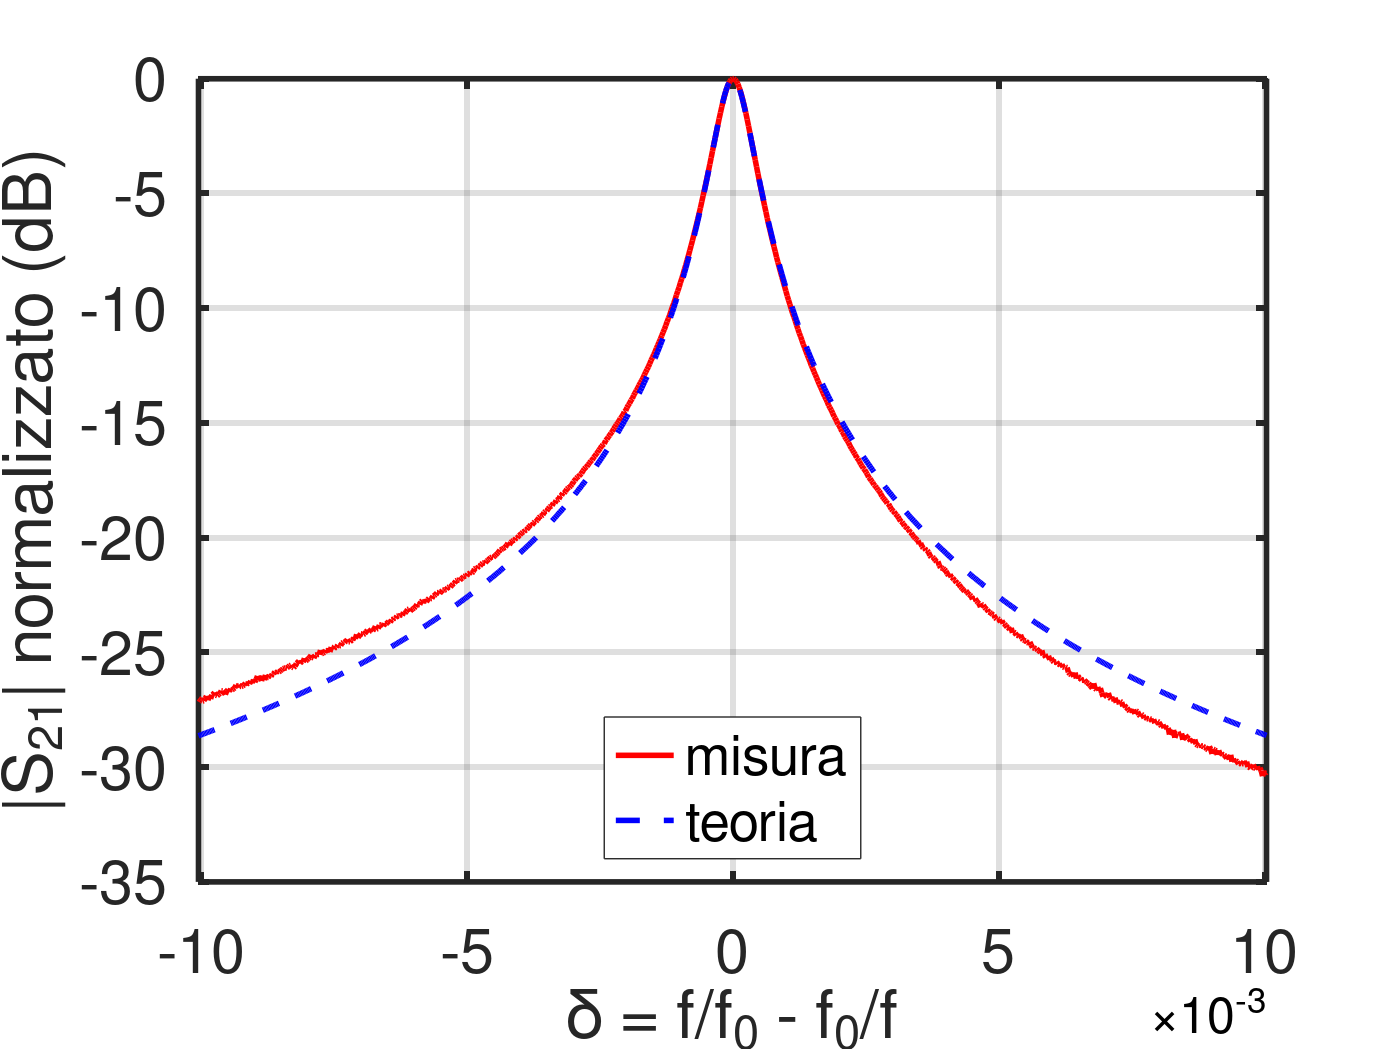
\includegraphics[width=\textwidth]{Images/Relazione6_Foto/fig_1_6_modo4.png}
\caption{modo 4 (normalizzato)}
\end{subfigure}
\caption{$|S_{21}(\delta)|$ in dB: misura e (\ref{eq:S21}) con $f_0$, $Q_L$ (quindi $Q_0$), $\beta_1$ e $\beta_2$ misurati. Per i modi 1 e 2 è riportata anche la misura corretta per le perdite dei cavi.}
\label{fig:16}
\end{figure}

Per il modo 1 la (\ref{eq:S21f0}) dà $|S_{21}(f_0)|=2\sqrt{0.491\cdot0.309}/1.800=0.433$, cioè $-7.27$\,dB, e dalla misurazione otteniamo $-10.79$\,dB; per il modo 2 il valore atteso è $-7.58$\,dB e quello misurato $-9.84$\,dB. La differenza di 2--3.5\,dB è dovuta soprattutto ai cavi, visto che la misura non è calibrata. L'attenuazione dei cavi la possiamo stimare dai livelli di $S_{11}$ e $S_{22}$ fuori risonanza, che corrispondono all'andata e al ritorno su ciascun cavo: in trasmissione il segnale attraversa una volta ciascun cavo, quindi l'attenuazione è circa la media dei due livelli, 2.80\,dB per il modo 1 e 2.91\,dB per il modo 2. Aggiungendo queste perdite, $|S_{21}(f_0)|$ misurato diventa $-7.98$\,dB per il modo 1 e $-6.93$\,dB per il modo 2, a 0.7\,dB dal valore atteso, una volta per difetto e una per eccesso. Questa stima delle perdite è approssimata, poiché il livello fuori risonanza contiene anche le code degli altri modi, come si vede vicino al modo 2 dove la traccia di $S_{22}$ sale di 0.4\,dB da sinistra a destra, e il disadattamento fra cavi e porte, che senza calibrazione non viene corretto. Una differenza di qualche decimo di dB è quindi ragionevole. Per un confronto vero sul valore assoluto servirebbe la misura calibrata, come dice la scheda.

La forma della curva è comunque quella attesa: vicino alla risonanza la misura corretta segue la teoria, e sulle code valgono le stesse osservazioni del punto 1.3 sui modi vicini.

\chapter{Tabella riassuntiva dei quattro modi}
\label{cap:riepilogo}

In tabella~\ref{tab:riepilogo} riportiamo i risultati della prima parte, come chiede il punto 1.7: la frequenza di risonanza, il $Q_L$ letto sullo strumento con la funzione automatica \emph{Bandwidth}, il $Q_L$ dalla banda a $-3$\,dB calcolato sulle tracce salvate, il $Q_L$ dal fit lineare della fase e, per i primi due modi, i coefficienti di accoppiamento e $Q_0$.

\begin{table}[H]
\centering
\renewcommand{\arraystretch}{1.3}
\setlength{\tabcolsep}{4pt}
\small
\begin{tabular}{c c c c c c c c}
\hline
 & $f_0$ & $Q_L$ & $Q_L$ & $Q_L$ & & & \\
modo & [GHz] & strumento & $|S_{21}|$, $-3$\,dB & $\angle S_{21}$, fit & $\beta_1$ & $\beta_2$ & $Q_0$ \\ \hline
1 & $1.939663(2)$ & 8274 & $8271 \pm 144$ & $8251 \pm 242$ & $0.491(4)$ & $0.309(5)$ & $14888 \pm 266$ \\
2 & $1.964197(8)$ & 7236 & $7240 \pm 409$ & $7229 \pm 174$ & $0.502(4)$ & $0.274(5)$ & $12863 \pm 728$ \\
3 & $2.858146(8)$ & 4240 & $4241 \pm 96$  & $4223 \pm 39$  & -- & -- & -- \\
4 & $2.986376(8)$ & 2680 & $2685 \pm 37$  & $2682 \pm 16$  & -- & -- & -- \\ \hline
\end{tabular}
\caption{Riepilogo delle misure sui quattro modi. Fra parentesi l'incertezza sull'ultima cifra.}
\label{tab:riepilogo}
\end{table}

Confrontando i tre valori di $Q_L$ di ciascun modo si nota che sono in accordo entro le incertezze, e le differenze fra modulo e fase sono al massimo dello 0.4\%. Il valore dal modulo ha l'incertezza più piccola quando nella banda cadono molti punti, come per il modo 1, mentre quello dalla fase è più preciso quando la risonanza è larga rispetto al passo, come per i modi 3 e 4. Per il modo 2, che ha pochi punti nella banda, il fit della fase dà un'incertezza più piccola della banda a $-3$\,dB, ma solo perché è statistica e non tiene conto della correzione di linearizzazione, che su $|Q_L\delta|\le1$ è grande, del 13\%. Nei modi 1 e 2 l'antenna 1 è accoppiata più dell'antenna 2 e $Q_0$ è circa 1.8 volte $Q_L$.

\chapter{Effetto dei tuner sul primo modo}
\label{cap:tuner}

In questa parte, il punto 2 della scheda, abbiamo considerato solo il primo modo della cavità, a circa 1.9397\,GHz, e siamo andati a vedere come cambiano la frequenza di risonanza e il fattore di merito caricato quando si inseriscono i due tuner, cioè due viti metalliche che entrano nella cavità. Per questa misurazione la calibrazione non è necessaria.

\section{Teorema di Slater}
Dalla teoria sappiamo che inserire un tuner equivale a togliere alla cavità un piccolo volume $\Delta V$, che viene occupato dal metallo, e che per il teorema di Slater la variazione relativa della frequenza di risonanza è
\begin{equation}
\frac{\Delta f}{f_0}=\frac{\int_{\Delta V}\left(\mu_0|\mathbf H|^2-\varepsilon_0|\mathbf E|^2\right)dV}{\int_{V}\left(\mu_0|\mathbf H|^2+\varepsilon_0|\mathbf E|^2\right)dV},
\label{eq:slater}
\end{equation}
cioè la frequenza scende se il tuner entra in una zona dove domina l'energia elettrica e sale se entra dove domina l'energia magnetica. Nel primo modo il campo in ciascuna cella ha la struttura del TM$_{010}$: il campo elettrico è parallelo all'asse ed è massimo sull'asse; il campo magnetico gira attorno all'asse, è nullo sull'asse ed è massimo vicino alla parete laterale, dove il campo elettrico si annulla. Ci aspettiamo quindi che un tuner che entra vicino all'asse faccia scendere la frequenza, e che un tuner che entra dalla parete laterale la faccia salire.

\section{Procedura}
Per prima cosa, con i tuner nella posizione iniziale, abbiamo misurato $|S_{21}|$ e lo abbiamo salvato nella memoria dello strumento con \emph{Trace}, \emph{Math Memory}, \emph{Data}$\rightarrow$\emph{Memory}, in modo da poter controllare, sovrapponendo le due tracce, di essere tornati nella posizione iniziale. In questa configurazione $f_0=1.939697$\,GHz e $Q_L=8271$, come nel punto 1. La misura è la seguente:

\begin{figure}[H]
\centering
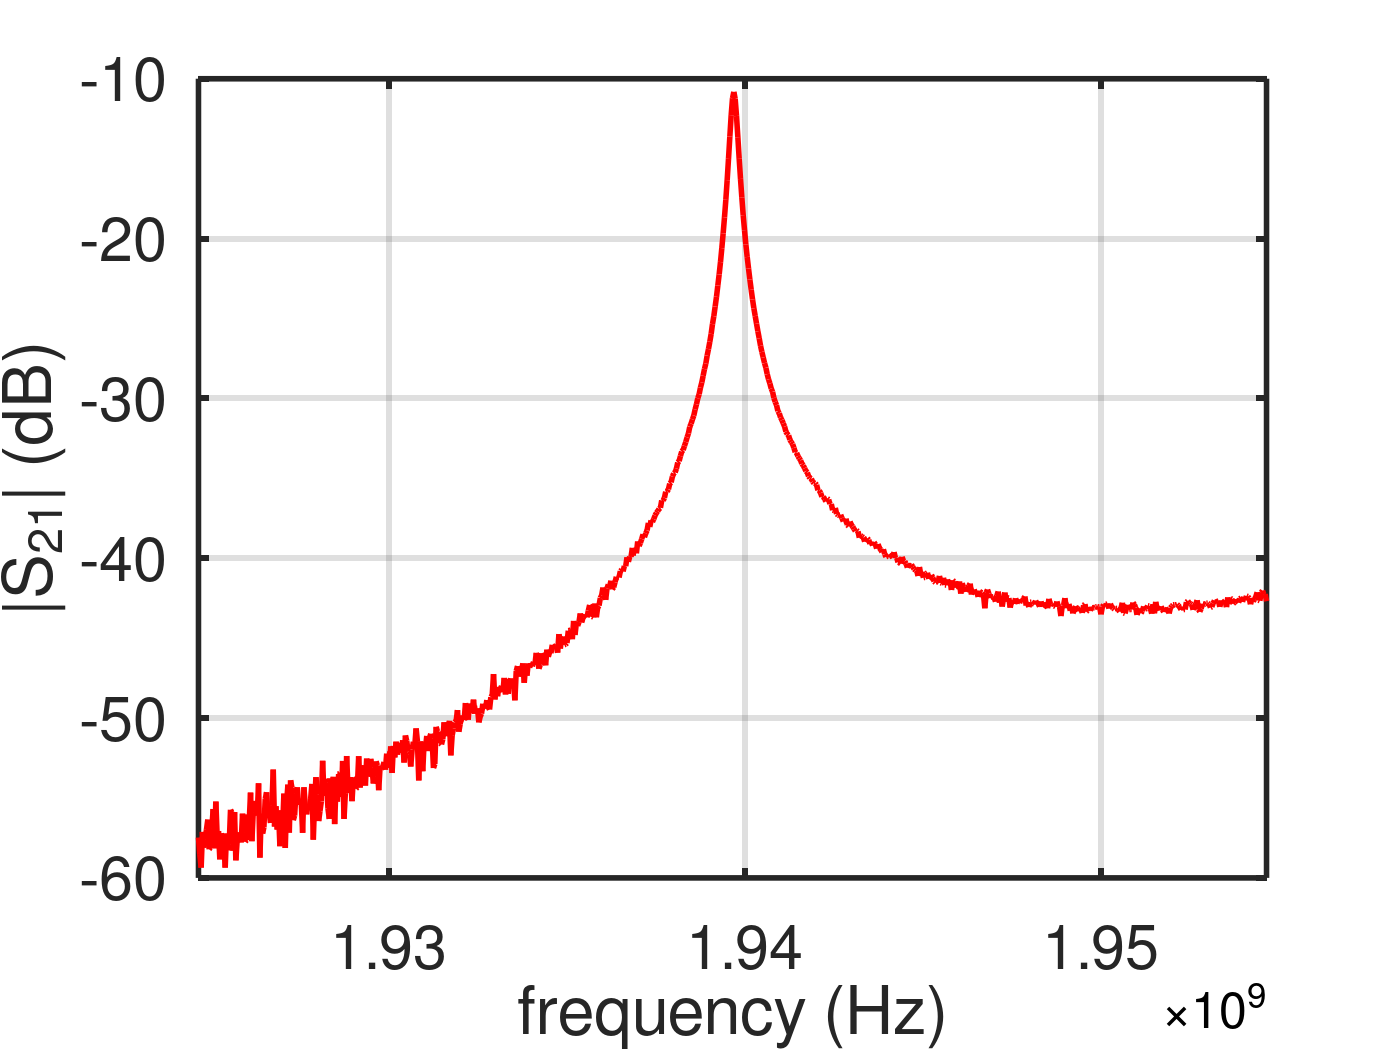
\includegraphics[width=0.6\textwidth]{Images/Relazione6_Foto/fig_2_1_iniziale.png}
\caption{Primo modo con i tuner nella posizione iniziale: modulo di $S_{21}$.}
\label{fig:21}
\end{figure}

Per leggere $f_0$ e $Q_L$ abbiamo usato la funzione \emph{Bandwidth} in modalità tracking, che li aggiorna a ogni sweep. La posizione dei tuner è contata in giri della vite a partire dalla posizione iniziale. Per ogni tuner abbiamo fatto 5 giri, uno alla volta, annotando $f_0$ e $Q_L$ dopo ogni giro, e poi lo abbiamo riportato nella posizione iniziale con 5 giri al contrario, controllando con la traccia in memoria, prima di passare all'altro. Per il primo tuner, che con 5 giri sposta la risonanza di circa 3\,MHz, abbiamo usato uno span da 1.934 a 1.943\,GHz, con la risonanza iniziale spostata verso destra per lasciare spazio allo spostamento.

\section{Risultati}
Le letture sono in tabella~\ref{tab:tuner} e nelle figure~\ref{fig:tunerf0} e~\ref{fig:tunerQ}. Dopo il primo giro del tuner 1 abbiamo annotato la frequenza solo fino alla quarta cifra decimale, 1.9394\,GHz, quindi quel punto ha un'incertezza di circa $\pm50$\,kHz; per il tuner 2 abbiamo annotato $Q_L$ solo in tre posizioni. Riportando il tuner 1 nella posizione iniziale la risonanza è tornata a 1.939653\,GHz, 44\,kHz sotto il valore di partenza: contando i giri la posizione si ritrova solo a meno di una frazione di giro, e per questo per il tuner 2 gli spostamenti sono calcolati rispetto a questo nuovo valore.

\begin{table}[H]
\centering
\renewcommand{\arraystretch}{1.2}
\begin{tabular}{c | c c c | c c c}
\hline
 & \multicolumn{3}{c|}{tuner 1} & \multicolumn{3}{c}{tuner 2} \\
giri & $f_0$ [GHz] & $\Delta f_0$ [kHz] & $Q_L$ & $f_0$ [GHz] & $\Delta f_0$ [kHz] & $Q_L$ \\ \hline
0 & 1.939697  & 0       & 8271 & 1.9396534 & 0      & 8293 \\
1 & 1.9394    & $-297$  & 8187 & 1.93966   & $+7$   & -- \\
2 & 1.939147  & $-550$  & 7907 & 1.9397404 & $+87$  & 8290 \\
3 & 1.9385498 & $-1147$ & 7832 & 1.9398190 & $+166$ & -- \\
4 & 1.937779  & $-1918$ & 7360 & 1.9399356 & $+282$ & 8240 \\
5 & 1.9367018 & $-2995$ & 7253 & 1.9400662 & $+413$ & -- \\ \hline
\end{tabular}
\caption{$f_0$ e $Q_L$ del primo modo in funzione dei giri dei due tuner.}
\label{tab:tuner}
\end{table}

\begin{figure}[H]
\centering
\begin{subfigure}{0.49\textwidth}\centering
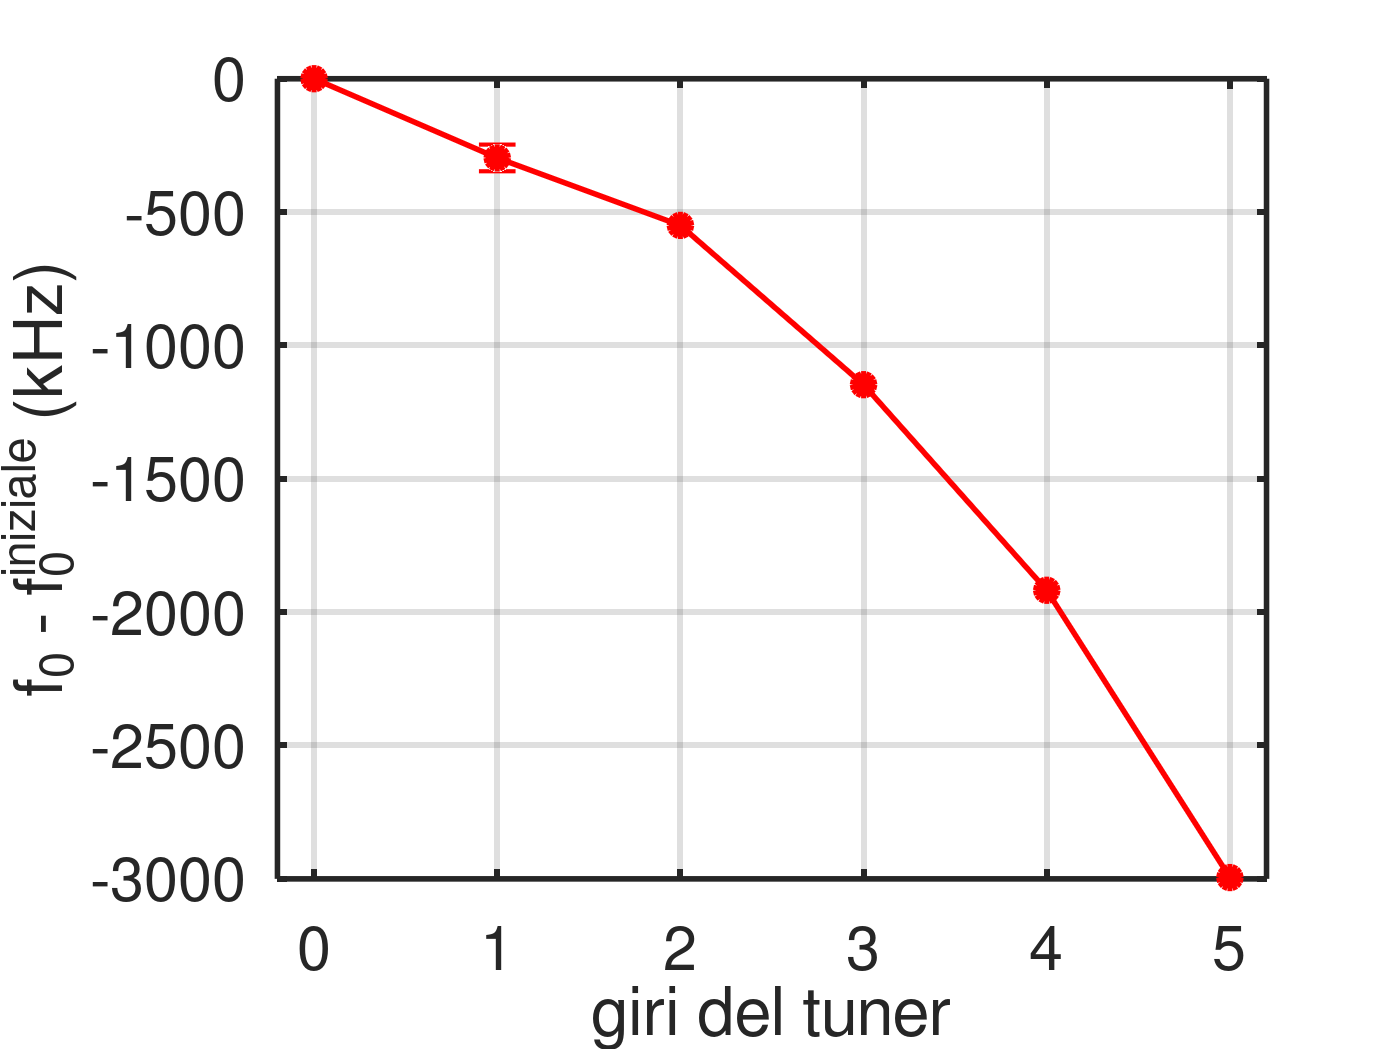
\includegraphics[width=\textwidth]{Images/Relazione6_Foto/fig_2_2_tuner1_f0.png}
\caption{tuner 1}
\end{subfigure}
\begin{subfigure}{0.49\textwidth}\centering
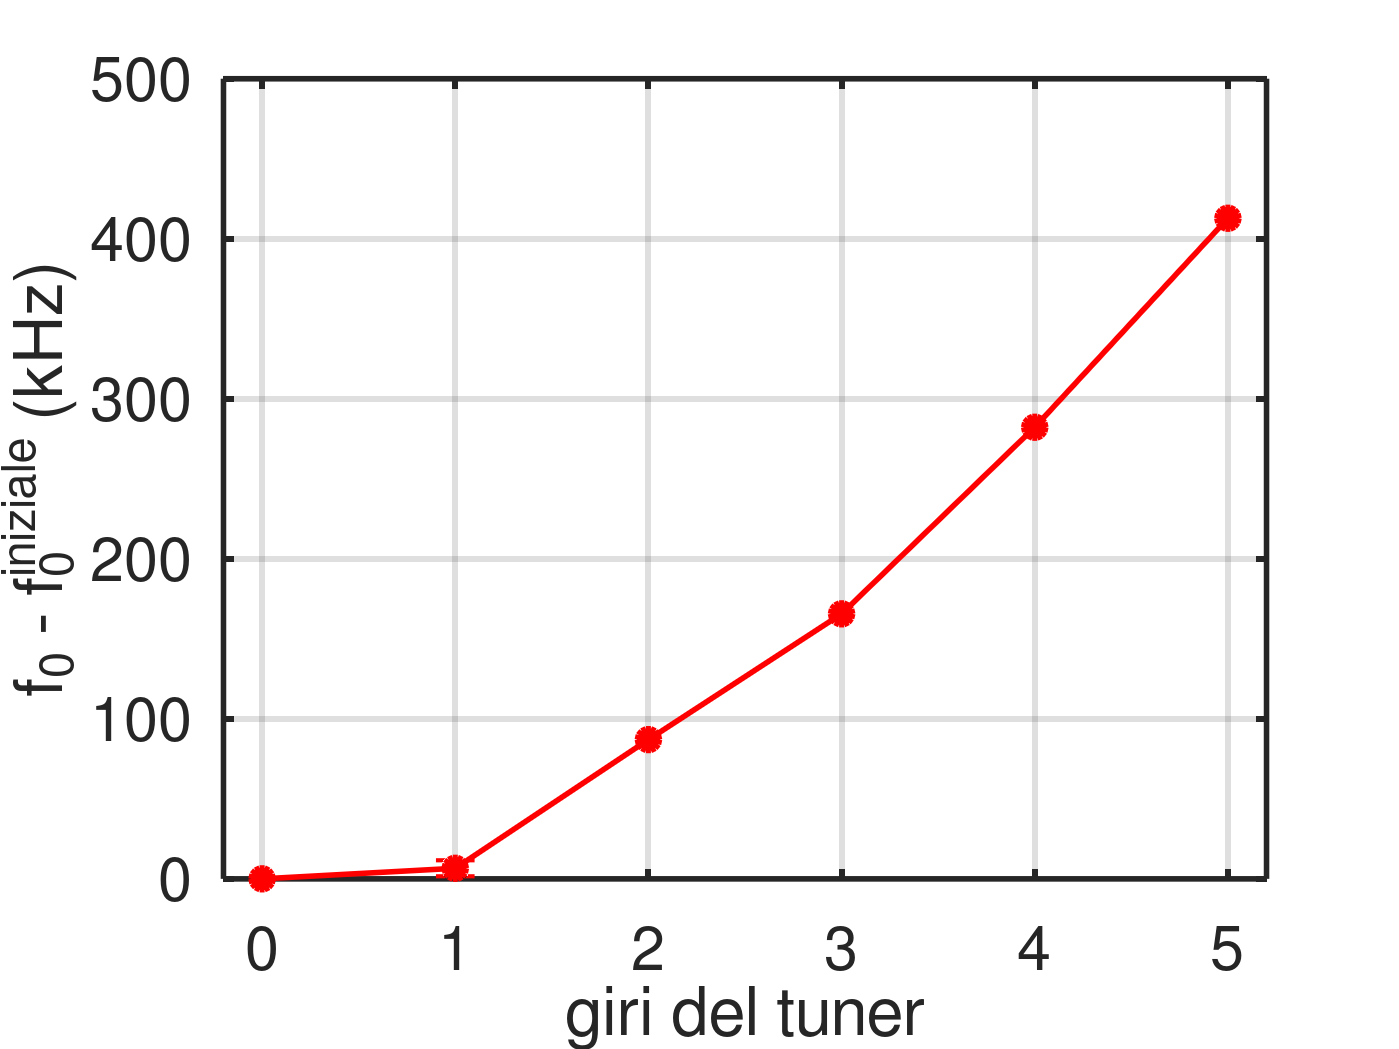
\includegraphics[width=\textwidth]{Images/Relazione6_Foto/fig_2_2_tuner2_f0.png}
\caption{tuner 2}
\end{subfigure}
\caption{Spostamento della frequenza di risonanza in funzione dei giri dei due tuner (attenzione alle scale diverse).}
\label{fig:tunerf0}
\end{figure}

\begin{figure}[H]
\centering
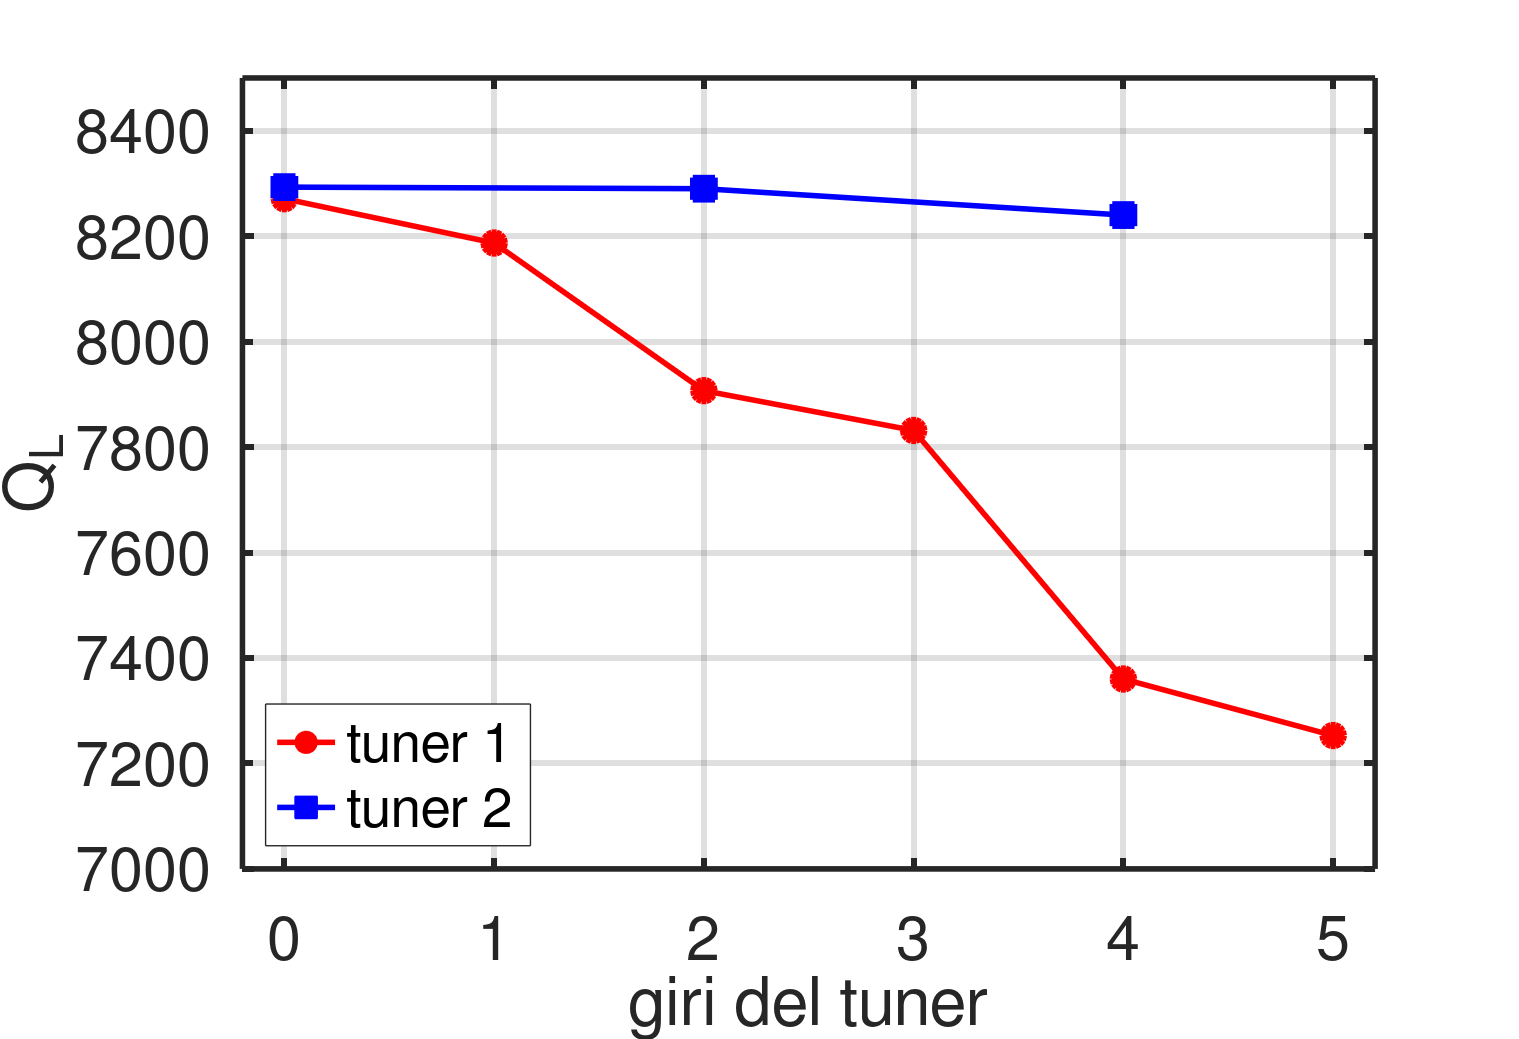
\includegraphics[width=0.6\textwidth]{Images/Relazione6_Foto/fig_2_2_QL.png}
\caption{$Q_L$ in funzione dei giri dei due tuner.}
\label{fig:tunerQ}
\end{figure}

\section{Commento}
Come si può notare, i due tuner spostano la frequenza in versi opposti. Il tuner 1 la fa scendere di circa 3\,MHz in 5 giri, e ogni giro sposta la risonanza più del precedente, da circa $-0.25$\,MHz per i primi giri a $-1.08$\,MHz per l'ultimo, perché la vite entra sempre più dentro, dove il campo elettrico è più intenso. Il tuner 2 invece fa salire la frequenza di 0.41\,MHz in 5 giri, cioè circa sette volte meno. Questo è proprio quello che prevede la (\ref{eq:slater}): il tuner 1 entra in una zona dove domina il campo elettrico e il tuner 2 in una zona dove domina il campo magnetico, vicino alla parete, dove il campo elettrico del modo è quasi nullo.

Anche $Q_L$ cambia in modo diverso: con il tuner 1 scende del 12\%, da 8271 a 7253, mentre con il tuner 2 resta praticamente costante, con variazioni fra 0 e $-0.6$\%. Un tuner aggiunge una superficie metallica su cui scorrono correnti, e quindi perdite, soprattutto nei contatti fra la vite e la parete. Il tuner 1, che sta dove il campo elettrico è forte e perturba di più il modo, cambia anche la distribuzione del campo vicino alle antenne e quindi può cambiare l'accoppiamento. Dalle sole letture di $Q_L$ non possiamo separare i due effetti, poiché non abbiamo salvato il livello di $|S_{21}|$ per ogni posizione. Va detto anche che con il tuner 1 inserito $Q_L$ oscillava parecchio da uno sweep all'altro: in una prima prova con 5 giri avevamo letto $f_0=1.936697$\,GHz e $Q_L=6909$, cioè la stessa frequenza entro 5\,kHz ma un $Q_L$ più basso del 5\%.

Possiamo quindi concludere che i tuner influenzano soprattutto la frequenza di risonanza, che è la grandezza per cui sono fatti, visto che servono ad accordare la cavità, e in misura minore $Q_L$. L'effetto sulla frequenza ha segno opposto per i due tuner perché il primo perturba il campo elettrico e il secondo il campo magnetico del modo.

\chapter{Cavità a due celle con accoppiamento simmetrico}
\label{cap:simm}
\chaptermark{Cavità a due celle}

Nella terza parte la cavità a due celle viene eccitata con le due antenne mobili, che permettono di variare il coefficiente di accoppiamento $\beta$ di ciascuna antenna. L'obiettivo è misurare $Q_0$ con le antenne il più possibile disaccoppiate e poi studiare la cavità con un accoppiamento simmetrico, confrontando i coefficienti di accoppiamento ricavati in modi diversi. Come chiede la scheda, con la correzione fatta in laboratorio, le misure le abbiamo fatte sul secondo modo di risonanza, a circa 1.964\,GHz, e non sul primo. Sullo strumento abbiamo visualizzato tre tracce nello stesso schermo, $S_{21}$, $S_{11}$ e $S_{22}$, centrate sulla risonanza con uno span di 2\,MHz, cioè 2.5\,kHz fra due punti.

Dalla teoria, nel caso di accoppiamento simmetrico con $\beta_1=\beta_2=\beta$, le (\ref{eq:S21f0}) diventano
\begin{equation}
S_{21}(f_0)=\frac{2\beta}{1+2\beta},\qquad Q_L=\frac{Q_0}{1+2\beta},
\label{eq:simm}
\end{equation}
da cui
\begin{equation}
\beta=\frac{S_{21}(f_0)}{2\left[1-S_{21}(f_0)\right]},\qquad \beta=\frac{1}{2}\left(\frac{Q_0}{Q_L}-1\right).
\label{eq:betasimm}
\end{equation}
Inoltre dalle (\ref{eq:deltaS}) con $\beta_1=\beta_2$ si ha $\Delta S_{11}=\Delta S_{22}=1/(1+2\beta)$, quindi alla risonanza deve valere $|S_{11}(f_0)|+|S_{21}(f_0)|=1$.

\section{Misura del secondo modo (punto 3.1)}
La scheda chiede di caricare la calibrazione a frequenza più bassa e di misurare bene in trasmissione il secondo modo. Prima di muovere le antenne abbiamo quindi misurato $|S_{21}|$ attorno al secondo modo su uno span di 15\,MHz, riportato in figura~\ref{fig:31}. La risonanza è a 1.964184\,GHz, con $|S_{21}|=-9.58$\,dB e $Q_L=7474\pm218$, valori compatibili con quelli del modo 2 nel capitolo~\ref{cap:modulo}. In questa misura, come in quella del punto 3.2, la calibrazione però non risultava attiva: nella fase di $S_{21}$ resta il ritardo dei cavi di circa 20\,ns. La calibrazione l'abbiamo richiamata solo prima del punto 3.3.

\begin{figure}[H]
\centering
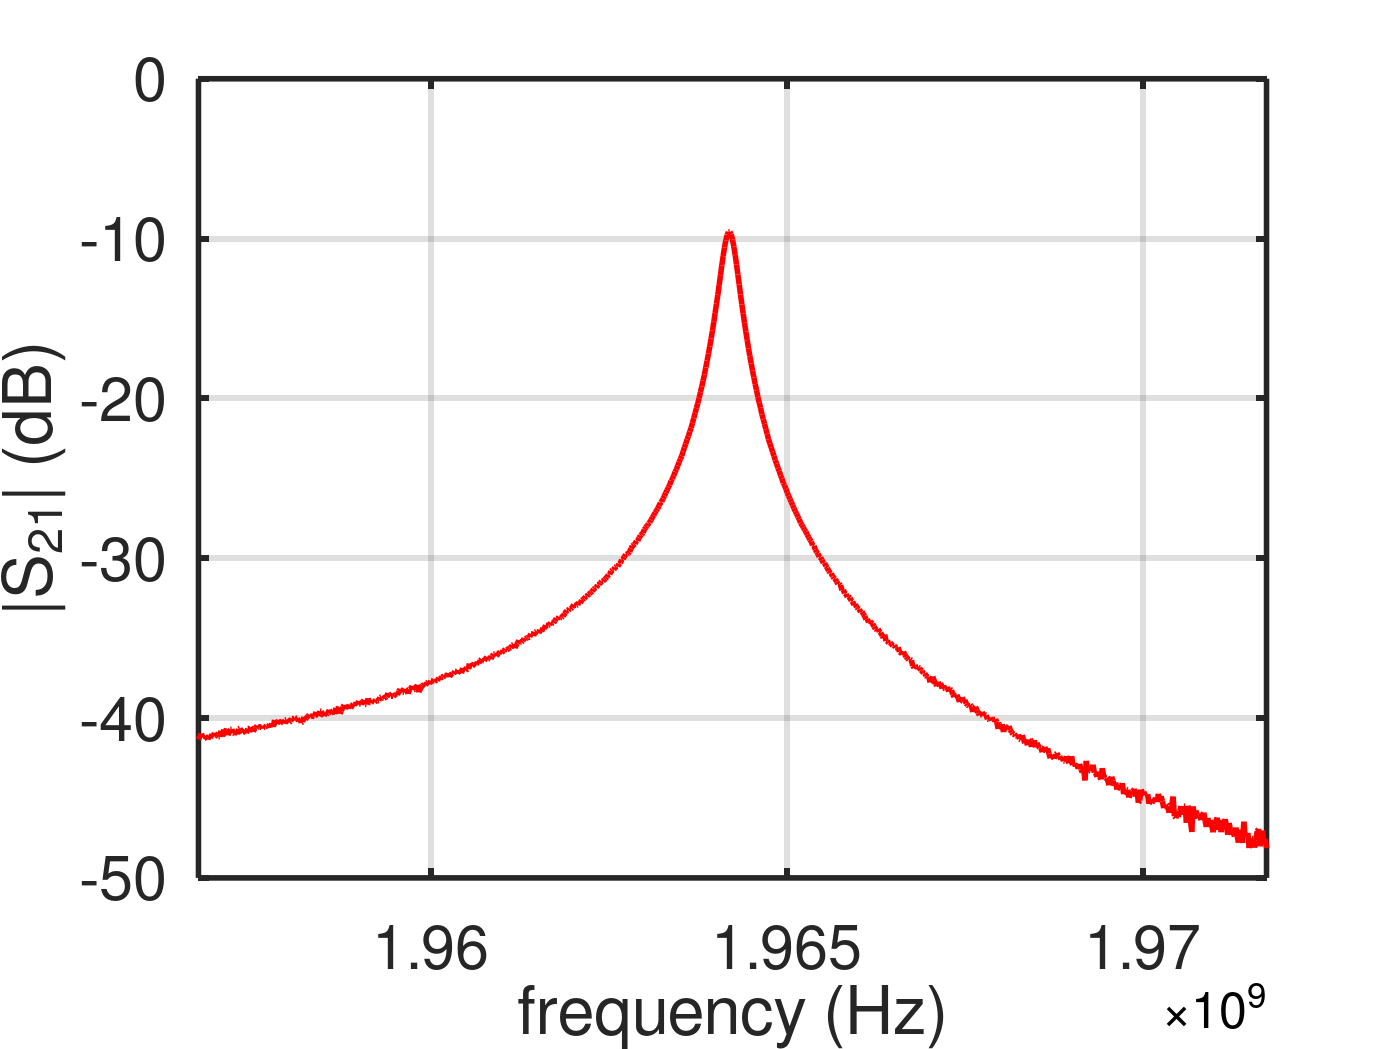
\includegraphics[width=0.6\textwidth]{Images/Relazione6_Foto/fig_3_1_S21.png}
\caption{Modulo di $S_{21}$ attorno al secondo modo prima di muovere le antenne.}
\label{fig:31}
\end{figure}

\section{$Q_0$ con le antenne disaccoppiate (punto 3.2)}
Siamo passati poi a estrarre le due antenne poco alla volta e in modo simmetrico, controllando che $S_{11}$ e $S_{22}$ restassero sottoaccoppiate, con buche sempre più piccole, finché il massimo di $|S_{21}|$ è sceso sotto $-40$\,dB. Solo a questo punto, come chiede la scheda, abbiamo ridotto la IF bandwidth, per avere una traccia più pulita. Le misure sono nelle figure~\ref{fig:32a} e~\ref{fig:32b}. Anche qui la calibrazione non era attiva: fuori risonanza $|S_{11}|$ vale circa $-2.6$\,dB e $|S_{22}|$ circa $-3.4$\,dB.

\begin{figure}[H]
\centering
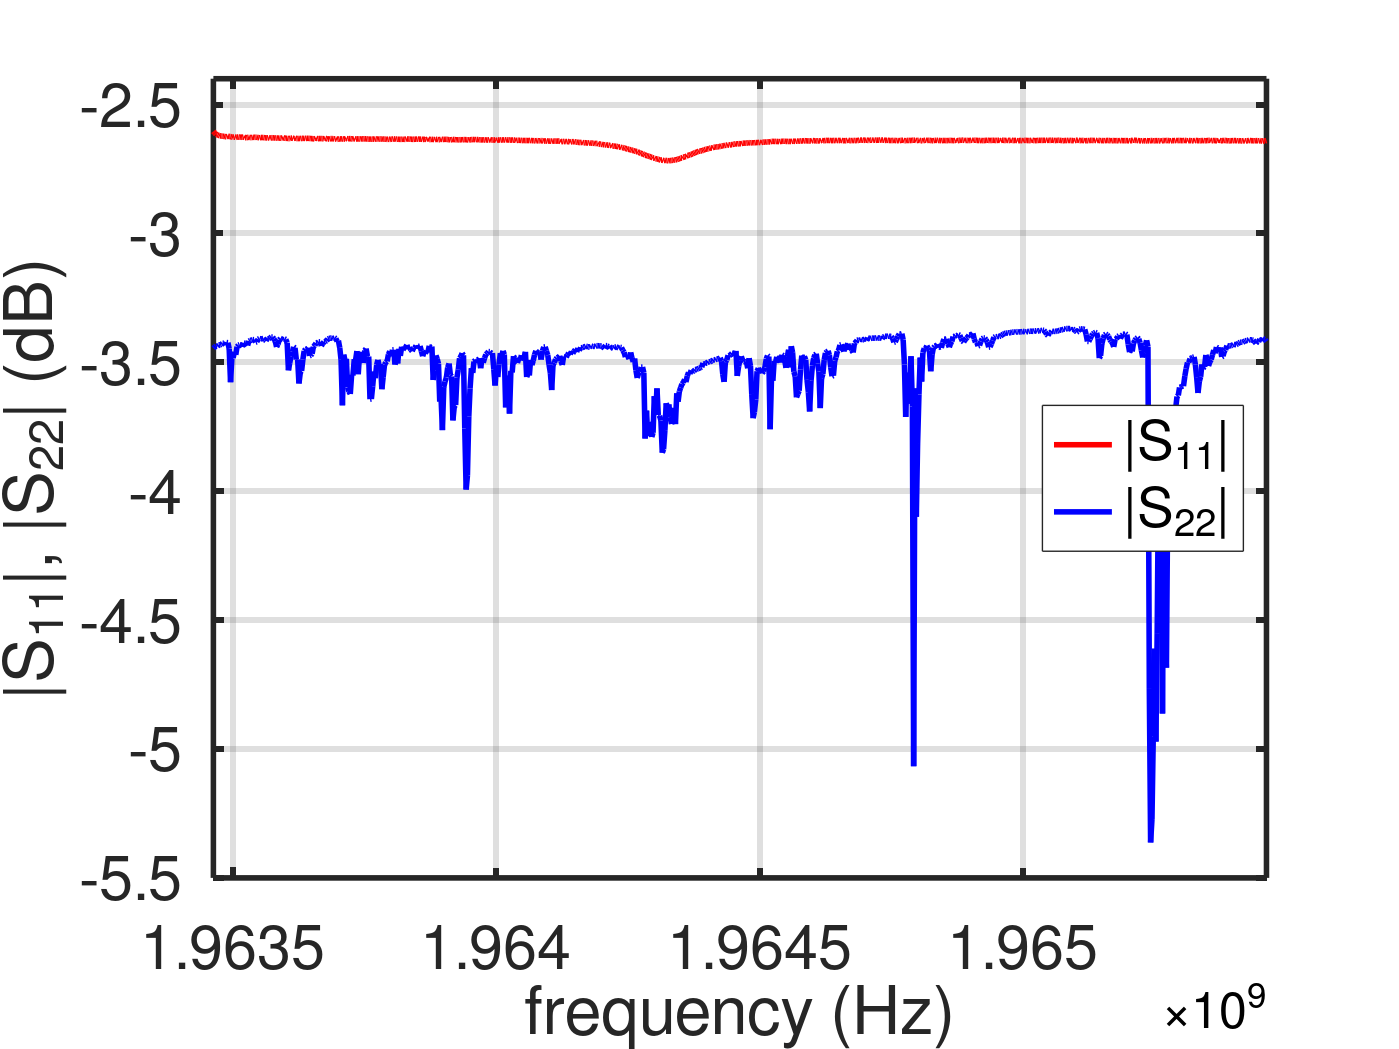
\includegraphics[width=0.6\textwidth]{Images/Relazione6_Foto/fig_3_2_S11_S22.png}
\caption{Antenne disaccoppiate: $|S_{11}|$ e $|S_{22}|$ sullo stesso grafico.}
\label{fig:32a}
\end{figure}

\begin{figure}[H]
\centering
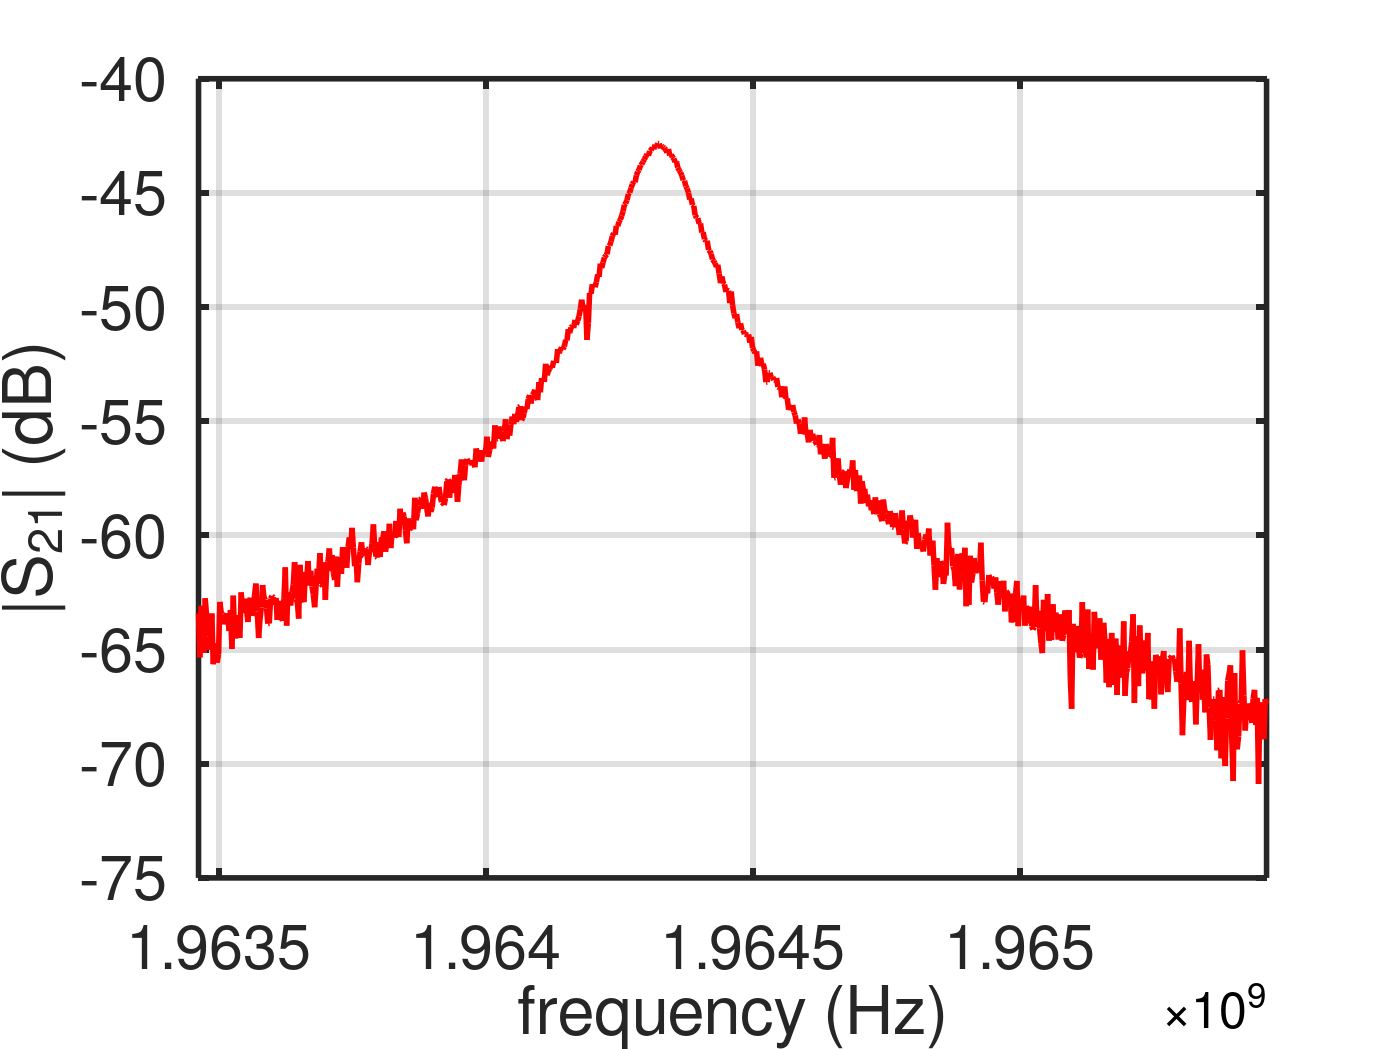
\includegraphics[width=0.6\textwidth]{Images/Relazione6_Foto/fig_3_2_S21.png}
\caption{Antenne disaccoppiate: $|S_{21}|$, con il massimo a $-42.8$\,dB.}
\label{fig:32b}
\end{figure}

Dalla banda a $-3$\,dB otteniamo $f_0=1.9643243$\,GHz, $BW=134.65$\,kHz e
\begin{equation}
Q_L=14589\pm111 ,
\end{equation}
con 54 punti dentro la banda. Siccome il picco è basso, abbiamo controllato questo valore anche con un fit della lorentziana su tutti i punti della traccia, che non dipende dal valore del singolo punto più alto: il fit dà $Q_L=14493\pm208$, in accordo con il valore precedente.

La buca di $S_{11}$ è di soli 0.08\,dB. Quella di $S_{22}$ in figura~\ref{fig:32a} non si distingue dal rumore, poiché questa traccia ha dei picchi verso il basso fino a 2\,dB, dovuti probabilmente a falsi contatti del connettore mentre muovevamo le antenne. Con le antenne simmetriche, da $\Delta S_{11}=10^{-0.082/20}=0.9906=1/(1+2\beta)$ si ha $\beta\simeq0.005$ per ciascuna antenna. Lo stesso ordine di grandezza si ottiene da $|S_{21}|$: aggiungendo circa 3\,dB di perdite dei cavi, cioè la media dei livelli di $S_{11}$ e $S_{22}$ fuori risonanza, il massimo diventa circa $-39.8$\,dB, e con questo valore di $\beta$ la (\ref{eq:simm}) dà $-40.5$\,dB. Quindi $Q_L$ coincide con $Q_0$ entro l'1\%:
\begin{equation}
Q_0=Q_L(1+2\beta)=14589\cdot1.0095\simeq14730\pm110 .
\end{equation}

\section{Accoppiamento simmetrico (punto 3.3)}
Poi abbiamo inserito le due antenne, alternandole, finché le buche di $|S_{11}|$ e $|S_{22}|$ sono diventate uguali fra loro e di circa 3\,dB rispetto al livello fuori risonanza, un po' meno dei 3.5\,dB indicati dalla scheda. Questa volta la calibrazione era attiva: infatti fuori risonanza $|S_{11}|$ e $|S_{22}|$ valgono ora $-0.35$ e $-0.05$\,dB e la fase non ha più la pendenza dovuta ai cavi. Le misure sono nelle figure~\ref{fig:33a} e~\ref{fig:33b}.

\begin{figure}[H]
\centering
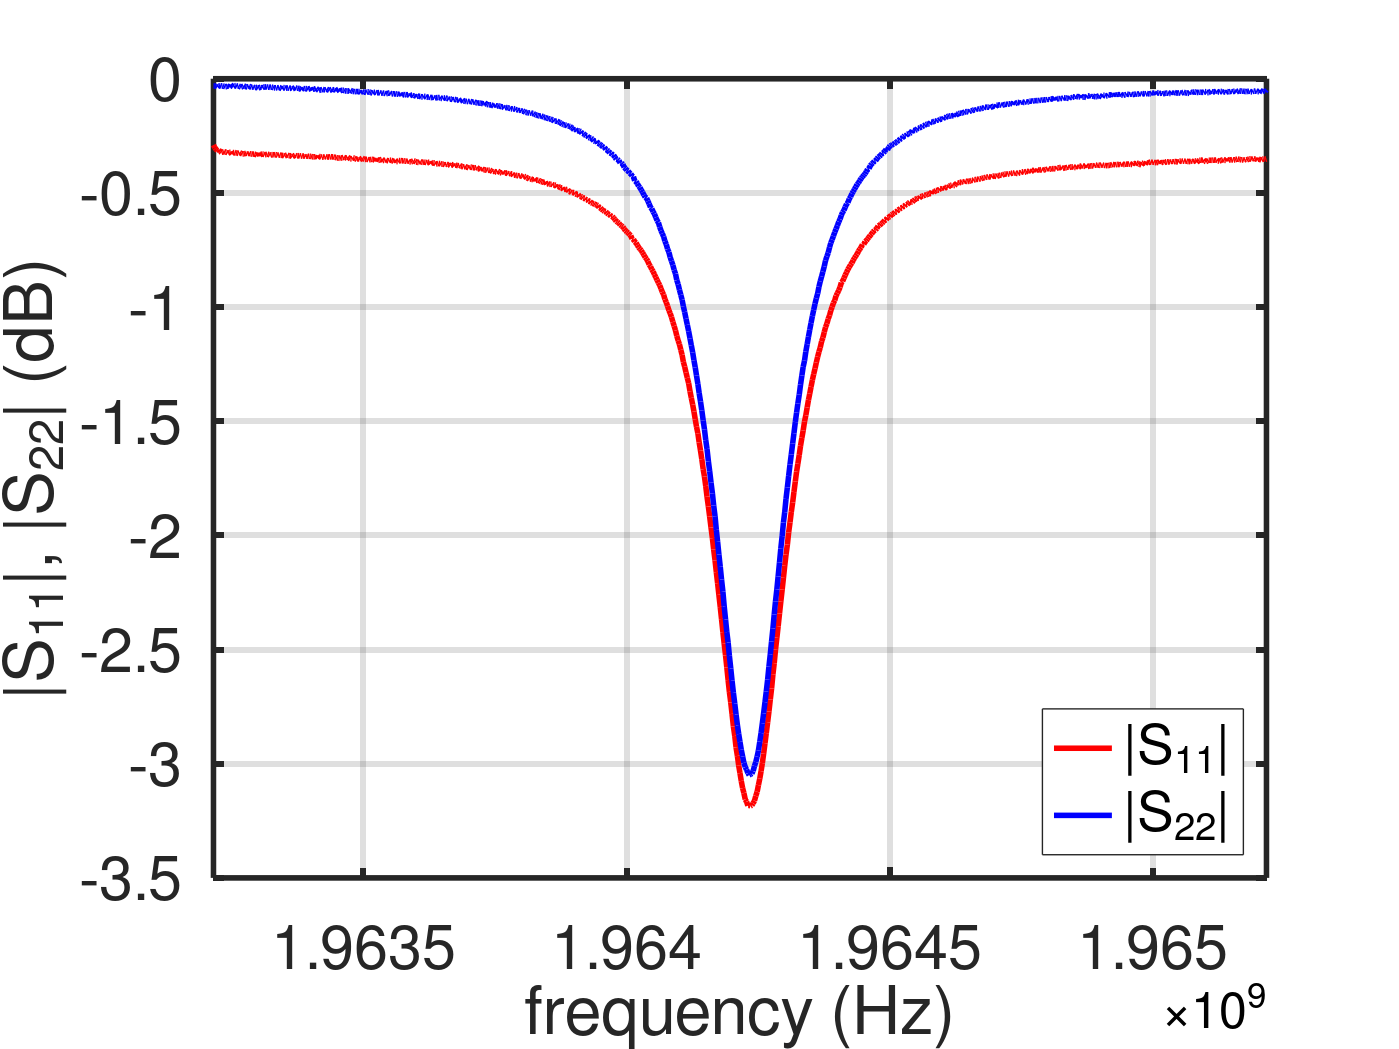
\includegraphics[width=0.6\textwidth]{Images/Relazione6_Foto/fig_3_3_S11_S22.png}
\caption{Accoppiamento simmetrico: $|S_{11}|$ e $|S_{22}|$ sullo stesso grafico.}
\label{fig:33a}
\end{figure}

\begin{figure}[H]
\centering
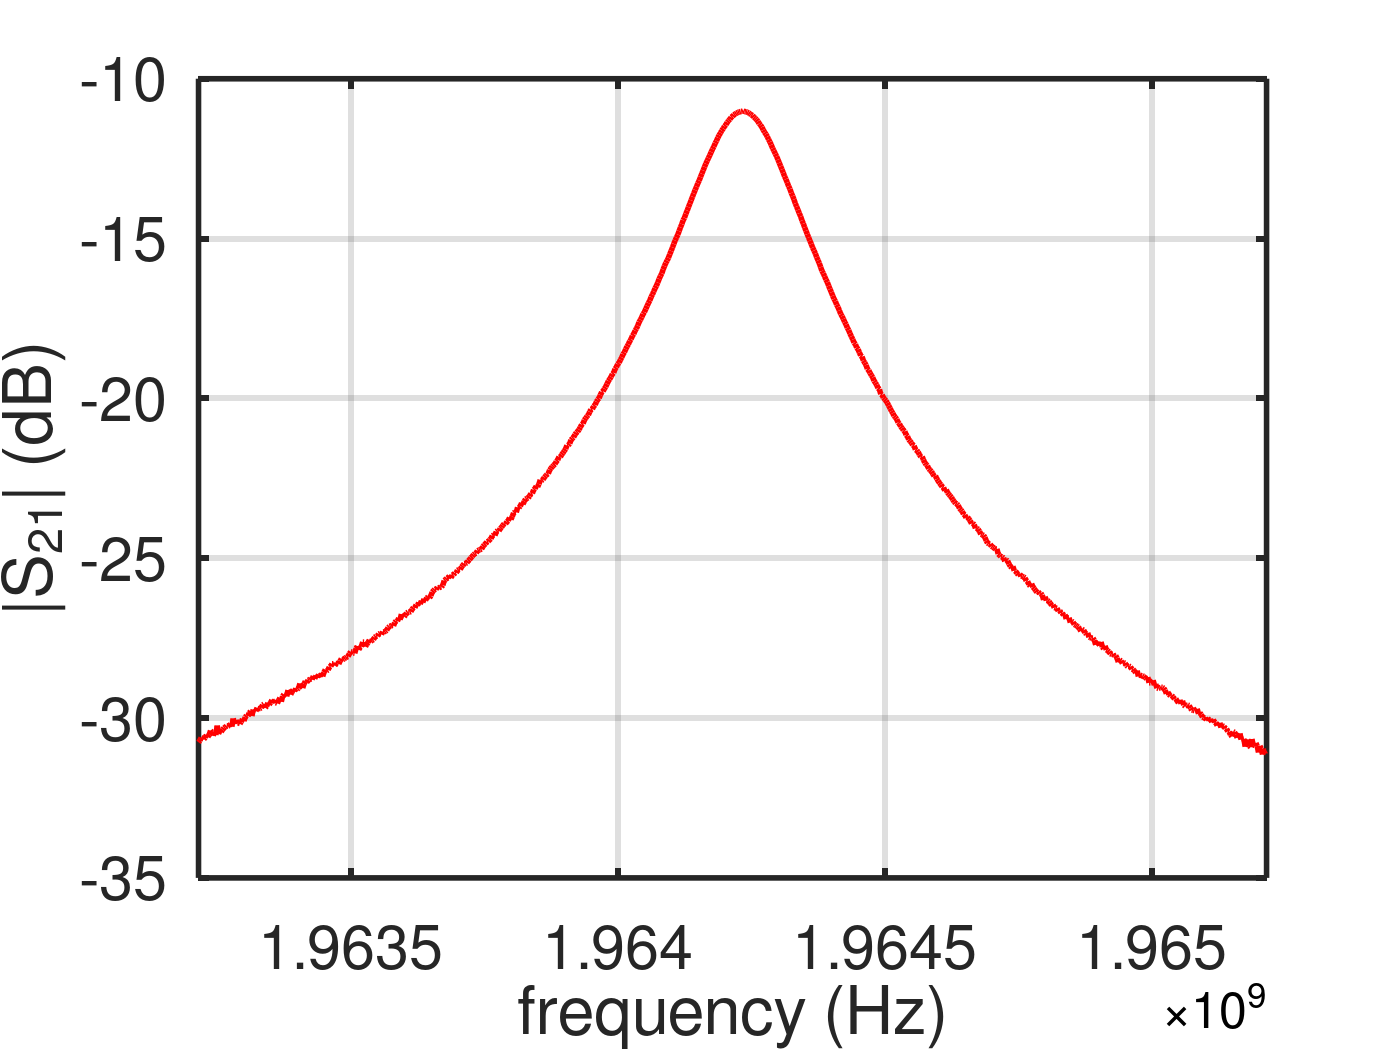
\includegraphics[width=0.6\textwidth]{Images/Relazione6_Foto/fig_3_3_S21.png}
\caption{Accoppiamento simmetrico: $|S_{21}|$.}
\label{fig:33b}
\end{figure}

Dalla traccia di $S_{21}$ otteniamo $f_0=1.9642340$\,GHz, $|S_{21}(f_0)|=-11.01$\,dB, $BW=202.62$\,kHz e
\begin{equation}
Q_L=9694\pm49
\end{equation}
con 81 punti nella banda. Sullo strumento la funzione \emph{Bandwidth} dava 9666, a 0.3\% dal nostro valore. Come ci aspettavamo $Q_L$ è più basso che nel punto 3.2, perché ora le antenne caricano la cavità. Per $S_{11}$ il livello fuori risonanza è $-0.348$\,dB e il minimo $-3.185$\,dB a 1.964235\,GHz, con una buca di 2.837\,dB; per $S_{22}$ il livello fuori risonanza è $-0.049$\,dB e il minimo $-3.050$\,dB, con una buca di 3.001\,dB. L'accoppiamento è quindi simmetrico entro 0.16\,dB.

\section{$\beta$ e $Q_0$ (punto 3.4)}
Con l'accoppiamento simmetrico possiamo ricavare $\beta$ in tre modi.
\begin{itemize}
\item Da $S_{21}(f_0)$: $|S_{21}(f_0)|=10^{-11.01/20}=0.2815$ e dalla (\ref{eq:betasimm}) $\beta=0.196\pm0.002$; con questo valore $Q_0=Q_L(1+2\beta)=13493\pm74$.
\item Dalle buche di $S_{11}$ e $S_{22}$, con le formule (\ref{eq:beta}) del corso: $\Delta S_{11}=0.7214$ e $\Delta S_{22}=0.7079$ danno $\beta_1=0.195\pm0.004$ e $\beta_2=0.204\pm0.004$ (media 0.200), e $Q_0=Q_L(1+\beta_1+\beta_2)=13566$.
\item Da $Q_0$ e $Q_L$: con il $Q_0$ misurato nel punto 3.2 e il $Q_L$ di questo punto, dalla (\ref{eq:betasimm}) $\beta=(14589/9694-1)/2=0.252\pm0.007$ (0.260 usando $Q_0=14730$).
\end{itemize}

I primi due metodi sono in ottimo accordo: $\beta$ da $S_{21}(f_0)$ cade fra $\beta_1$ e $\beta_2$, e i due $Q_0$ differiscono dello 0.5\%. Anche la verifica sulla somma funziona: $|S_{11}(f_0)|+|S_{21}(f_0)|=0.7214+0.2815=1.003$ e $|S_{22}(f_0)|+|S_{21}(f_0)|=0.989$, molto vicini a 1. Questo confronto ha senso solo perché in questo punto la misura era calibrata, ciò vuol dire che $|S_{21}(f_0)|$ non contiene le perdite dei cavi.

Il terzo metodo invece dà un $\beta$ più grande del 25--30\%. Il motivo è che usa il $Q_0$ misurato con le antenne estratte, 14730, ma con le antenne inserite il $Q_0$ che ricaviamo dagli altri due metodi è circa 13500, cioè l'8\% più basso: il $Q_0$ della cavità non rimane costante quando inseriamo le antenne. Probabilmente le antenne inserite di più portano più corrente sulla loro superficie e nei contatti, e quindi aggiungono perdite, oltre a perturbare il campo: lo si vede anche dalla frequenza di risonanza, che passa da 1.9643243\,GHz con le antenne estratte a 1.9642340\,GHz con l'accoppiamento simmetrico, 90\,kHz più in basso. La stessa tendenza si vede nel modo 2 della prima parte, misurato con le antenne ancora più inserite, con $\beta_1=0.50$ e $\beta_2=0.27$: lì $f_0=1.964197$\,GHz e $Q_0=12863\pm728$. Possiamo quindi concludere che, con le nostre antenne, $\beta$ calcolato da $Q_0/Q_L$ va preso con cautela, mentre i valori da $S_{21}(f_0)$ e dalle buche, che si riferiscono alla stessa configurazione, sono più affidabili.

\section{$|S_{21}(f)|$ misurato e teorico (punto 3.5)}
In figura~\ref{fig:35} è sovrapposta a $|S_{21}(f)|$ misurato in accoppiamento simmetrico la (\ref{eq:S21}), calcolata con $f_0$ e $Q_L$ misurati e con $S_{21}(f_0)$ dalla (\ref{eq:simm}), per due valori di $\beta$: 0.200, la media delle buche, e 0.252, quello da $Q_0/Q_L$.

\begin{figure}[H]
\centering
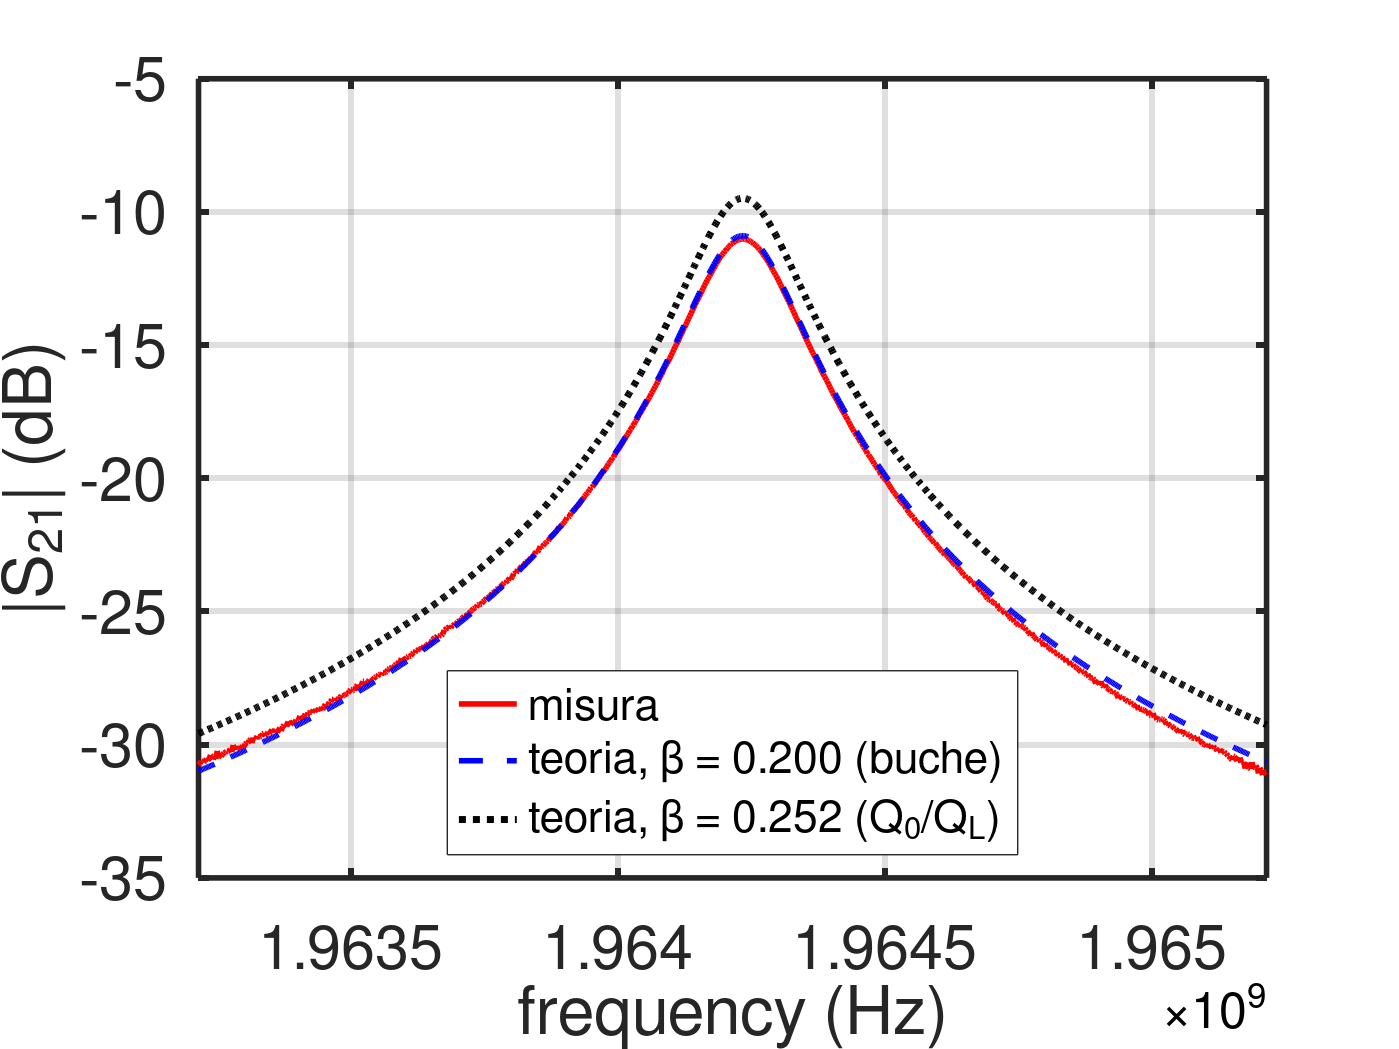
\includegraphics[width=0.7\textwidth]{Images/Relazione6_Foto/fig_3_5.png}
\caption{Accoppiamento simmetrico: $|S_{21}(f)|$ misurato e teorico con $\beta=0.200$ e $\beta=0.252$.}
\label{fig:35}
\end{figure}

Con $\beta=0.200$ la curva teorica si sovrappone bene alla misura: il massimo teorico è $-10.89$\,dB contro $-11.01$\,dB misurato e per $|Q_L\delta|\le1$ lo scarto medio è di 0.12\,dB. Con $\beta=0.252$ la curva ha la stessa forma ma sta 1.5\,dB più in alto, con il massimo a $-9.49$\,dB, per il motivo discusso nel punto precedente.

\end{document}
